\documentclass[../thesis.tex]{subfiles}
\begin{document}

\chapter{Parametric Study}
\label{chp: para_stud}
The parametric study is done, to distinguish between the influence of the thermophysical properties, against the one coming from convection on the front's shape and metrics. To achieve that different inlet velocities are used to investigate the influence of convection. To get the influence of the thermophysical properties different diffusion coefficients and viscosities are set. This results in the combination of parameters studied as shown in \autoref{tab: cases}.

Within the parametric study three different reactor geometries are simulated. The different conditions set for each case lead to different front shapes. Two of these front shapes for two example cases can be seen in \autoref{fig: shape_examp}.
\begin{figure}[htb]
	\centering
	\subfloat[\centering Front shape for  h = 0.6mm Pe = 2050 Sc = 12000]{{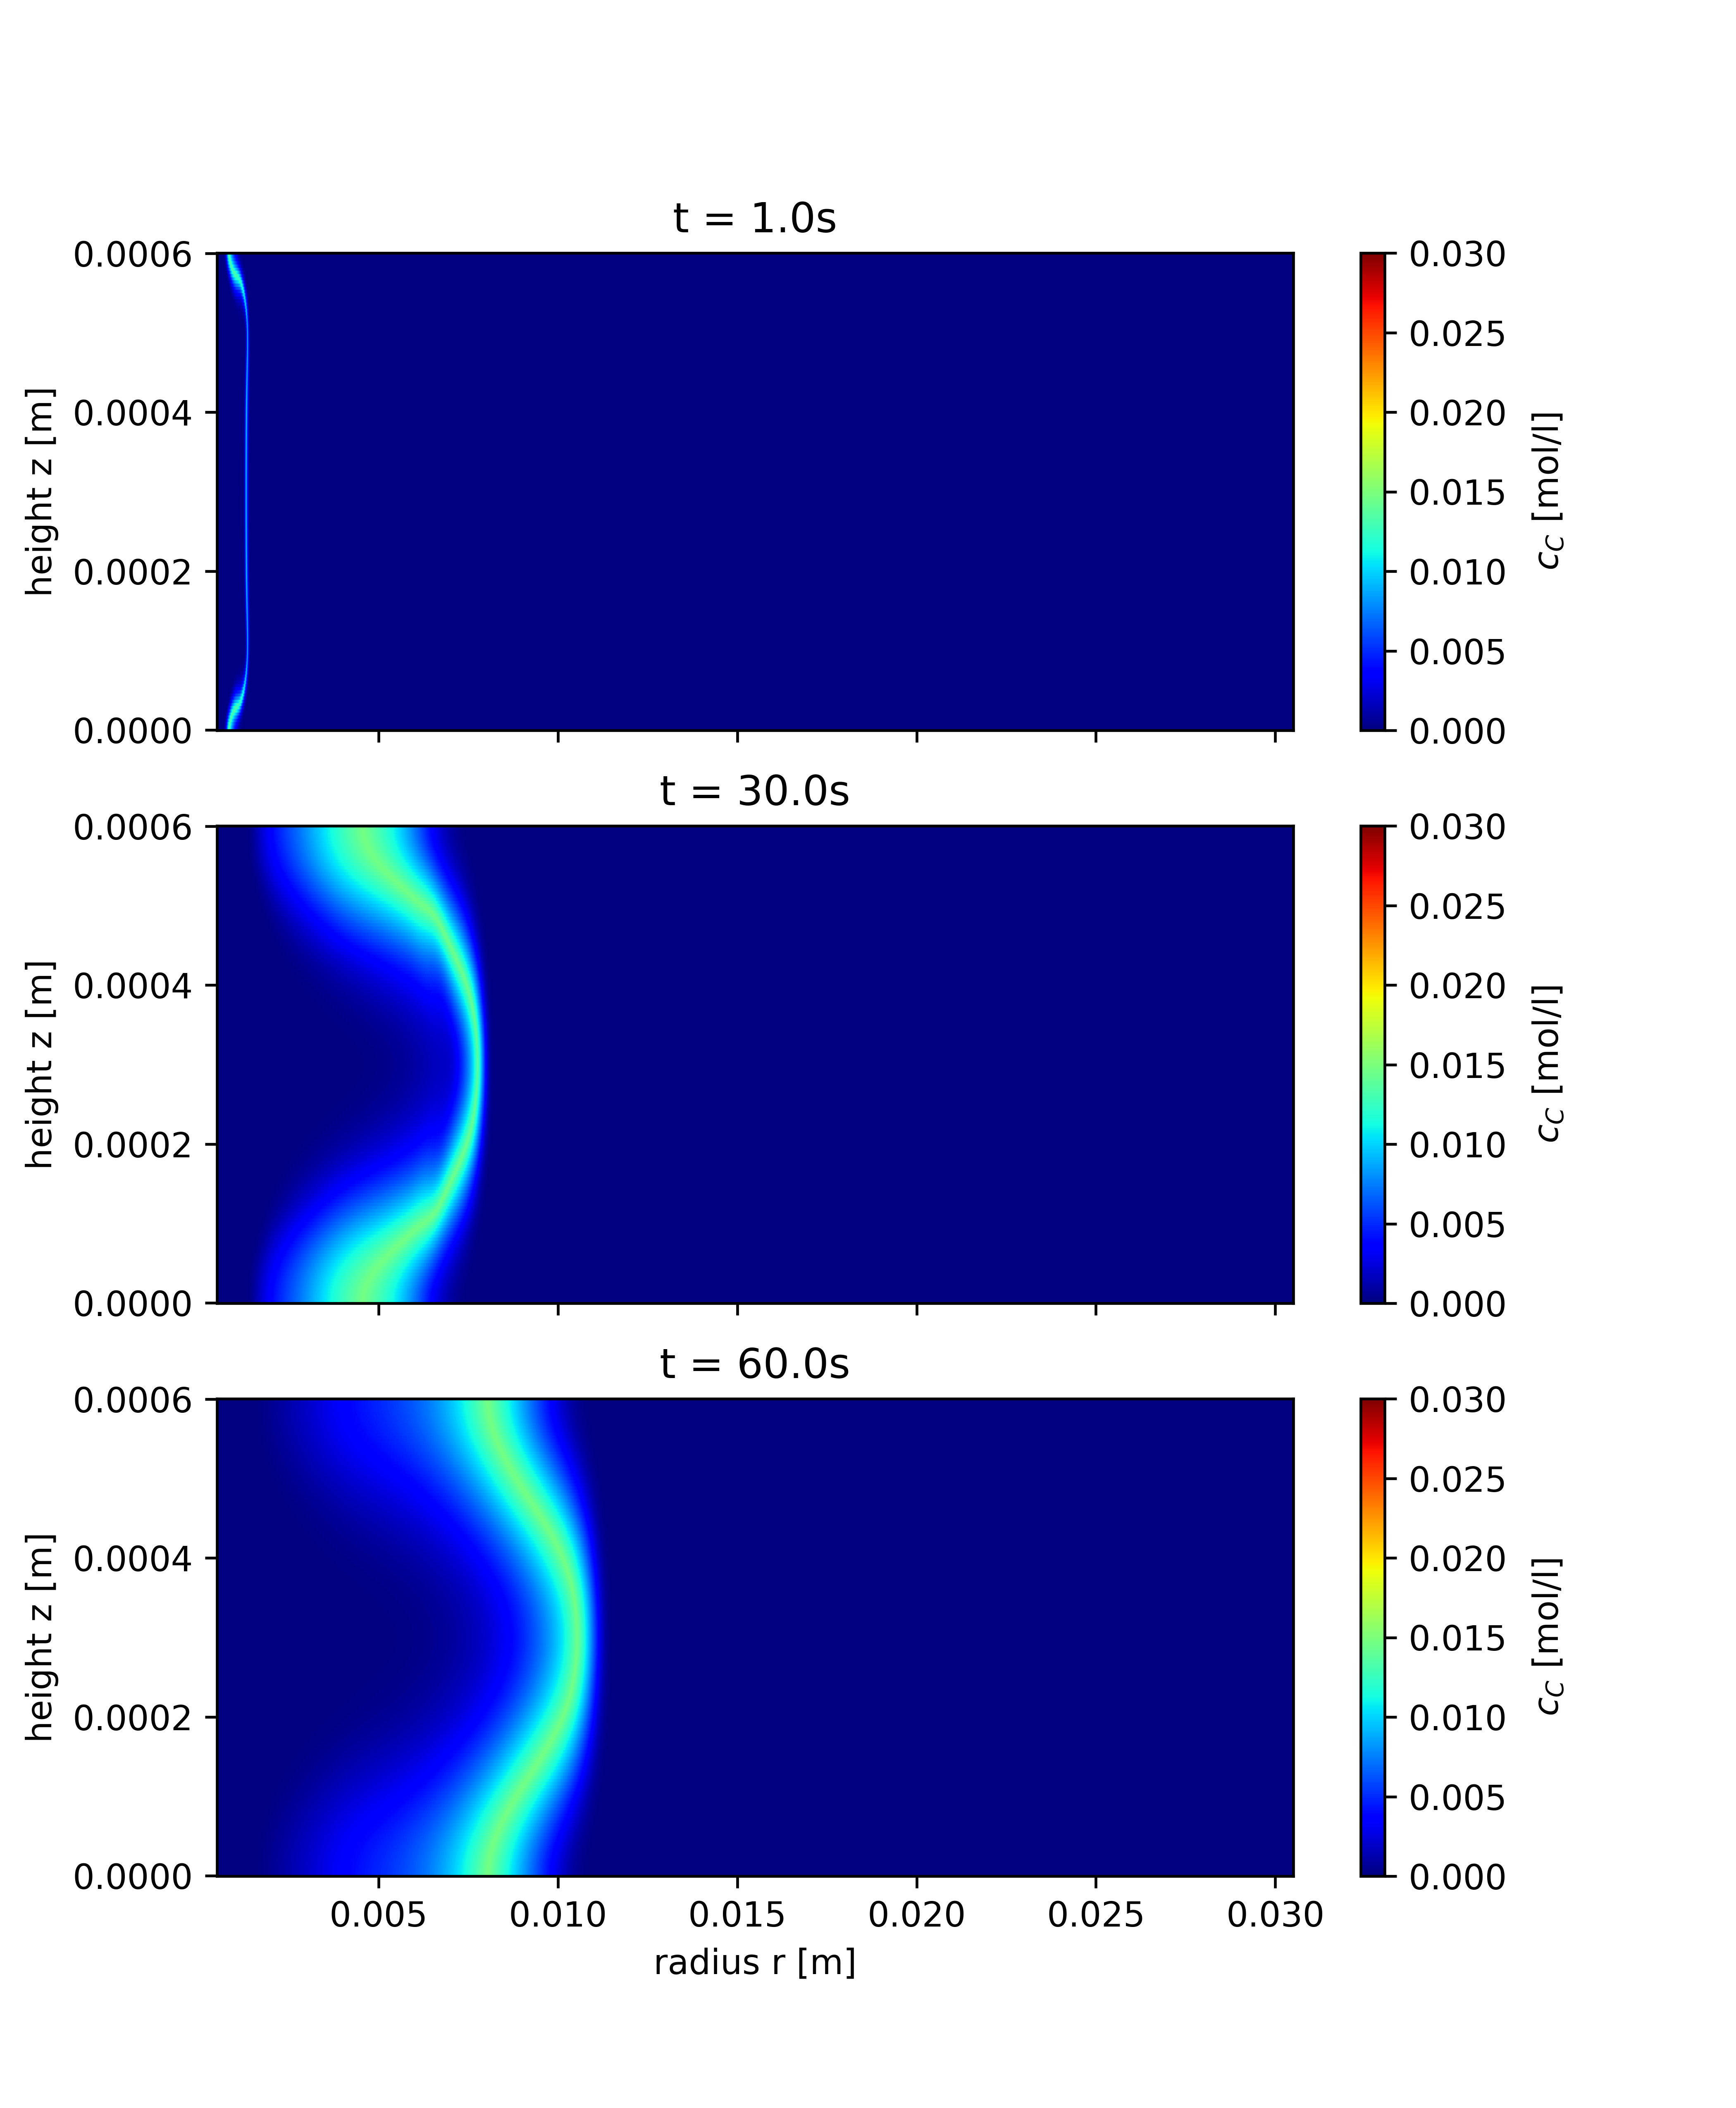
\includegraphics[angle=0, scale=0.41]{front_shape1} }}%
	\qquad
	\subfloat[\centering Front shape for  h = 0.2mm Pe = 2050 Sc = 2430]{{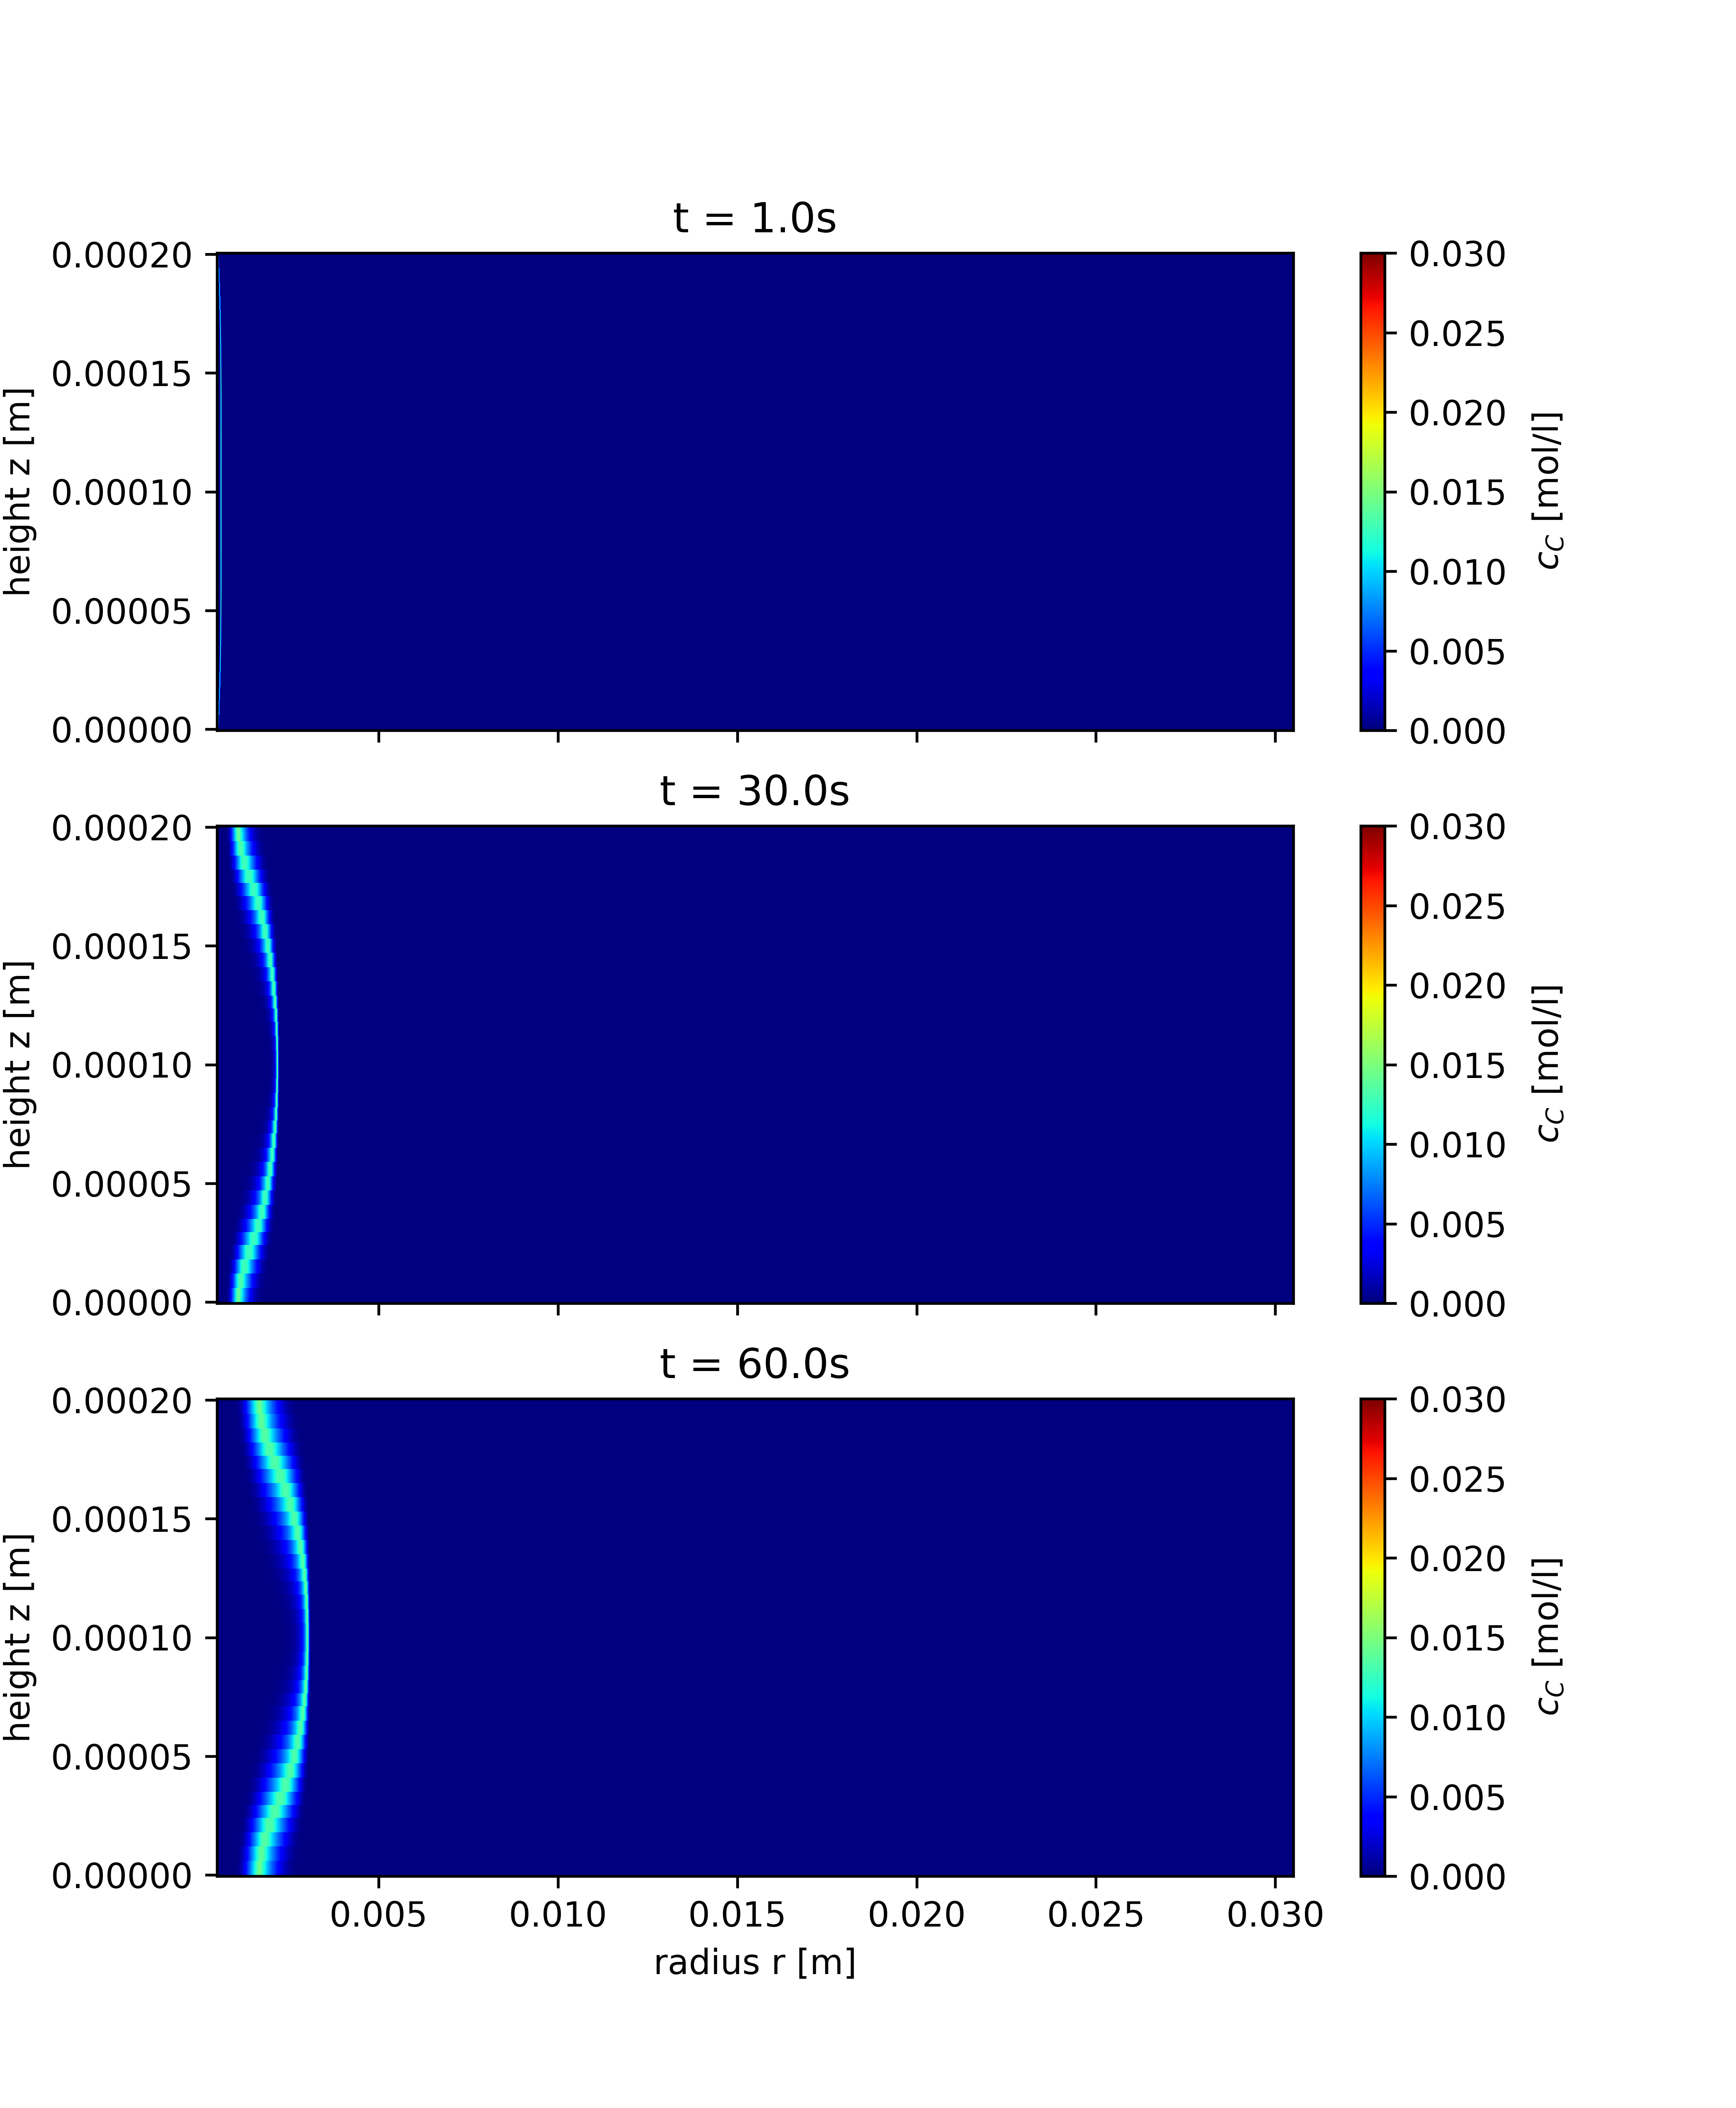
\includegraphics[angle=0, scale=0.41]{front_shape2} }}%
	\caption{Two example front shapes as a result of different flow conditions}%
	\label{fig: shape_examp}%
\end{figure}
Comparing the cases shown in \autoref{fig: shape_examp} it becomes clear, that the reactor gap height and thermophysical properties show a significant influence on the fronts progression and curvature. In addition to that the front's width is also influenced. A more detailed analysis of the front's position, width and the total amount of product formed is given in the following sections. 

\section{Front Positions}

The front positions behave in a similar way for all 3 reactor geometries. In \autoref{fig: front_pos_h2_Sc12000} and \autoref{fig: front_pos_h2_Sc2430} the positions for both Schmidt numbers are shown for the geometry containing a gap height of 0.2mm. The plots for the other two gap heights can be found in Section \ref{chp: app_frontpos}.
\begin{figure}[htbp]
	\centering
	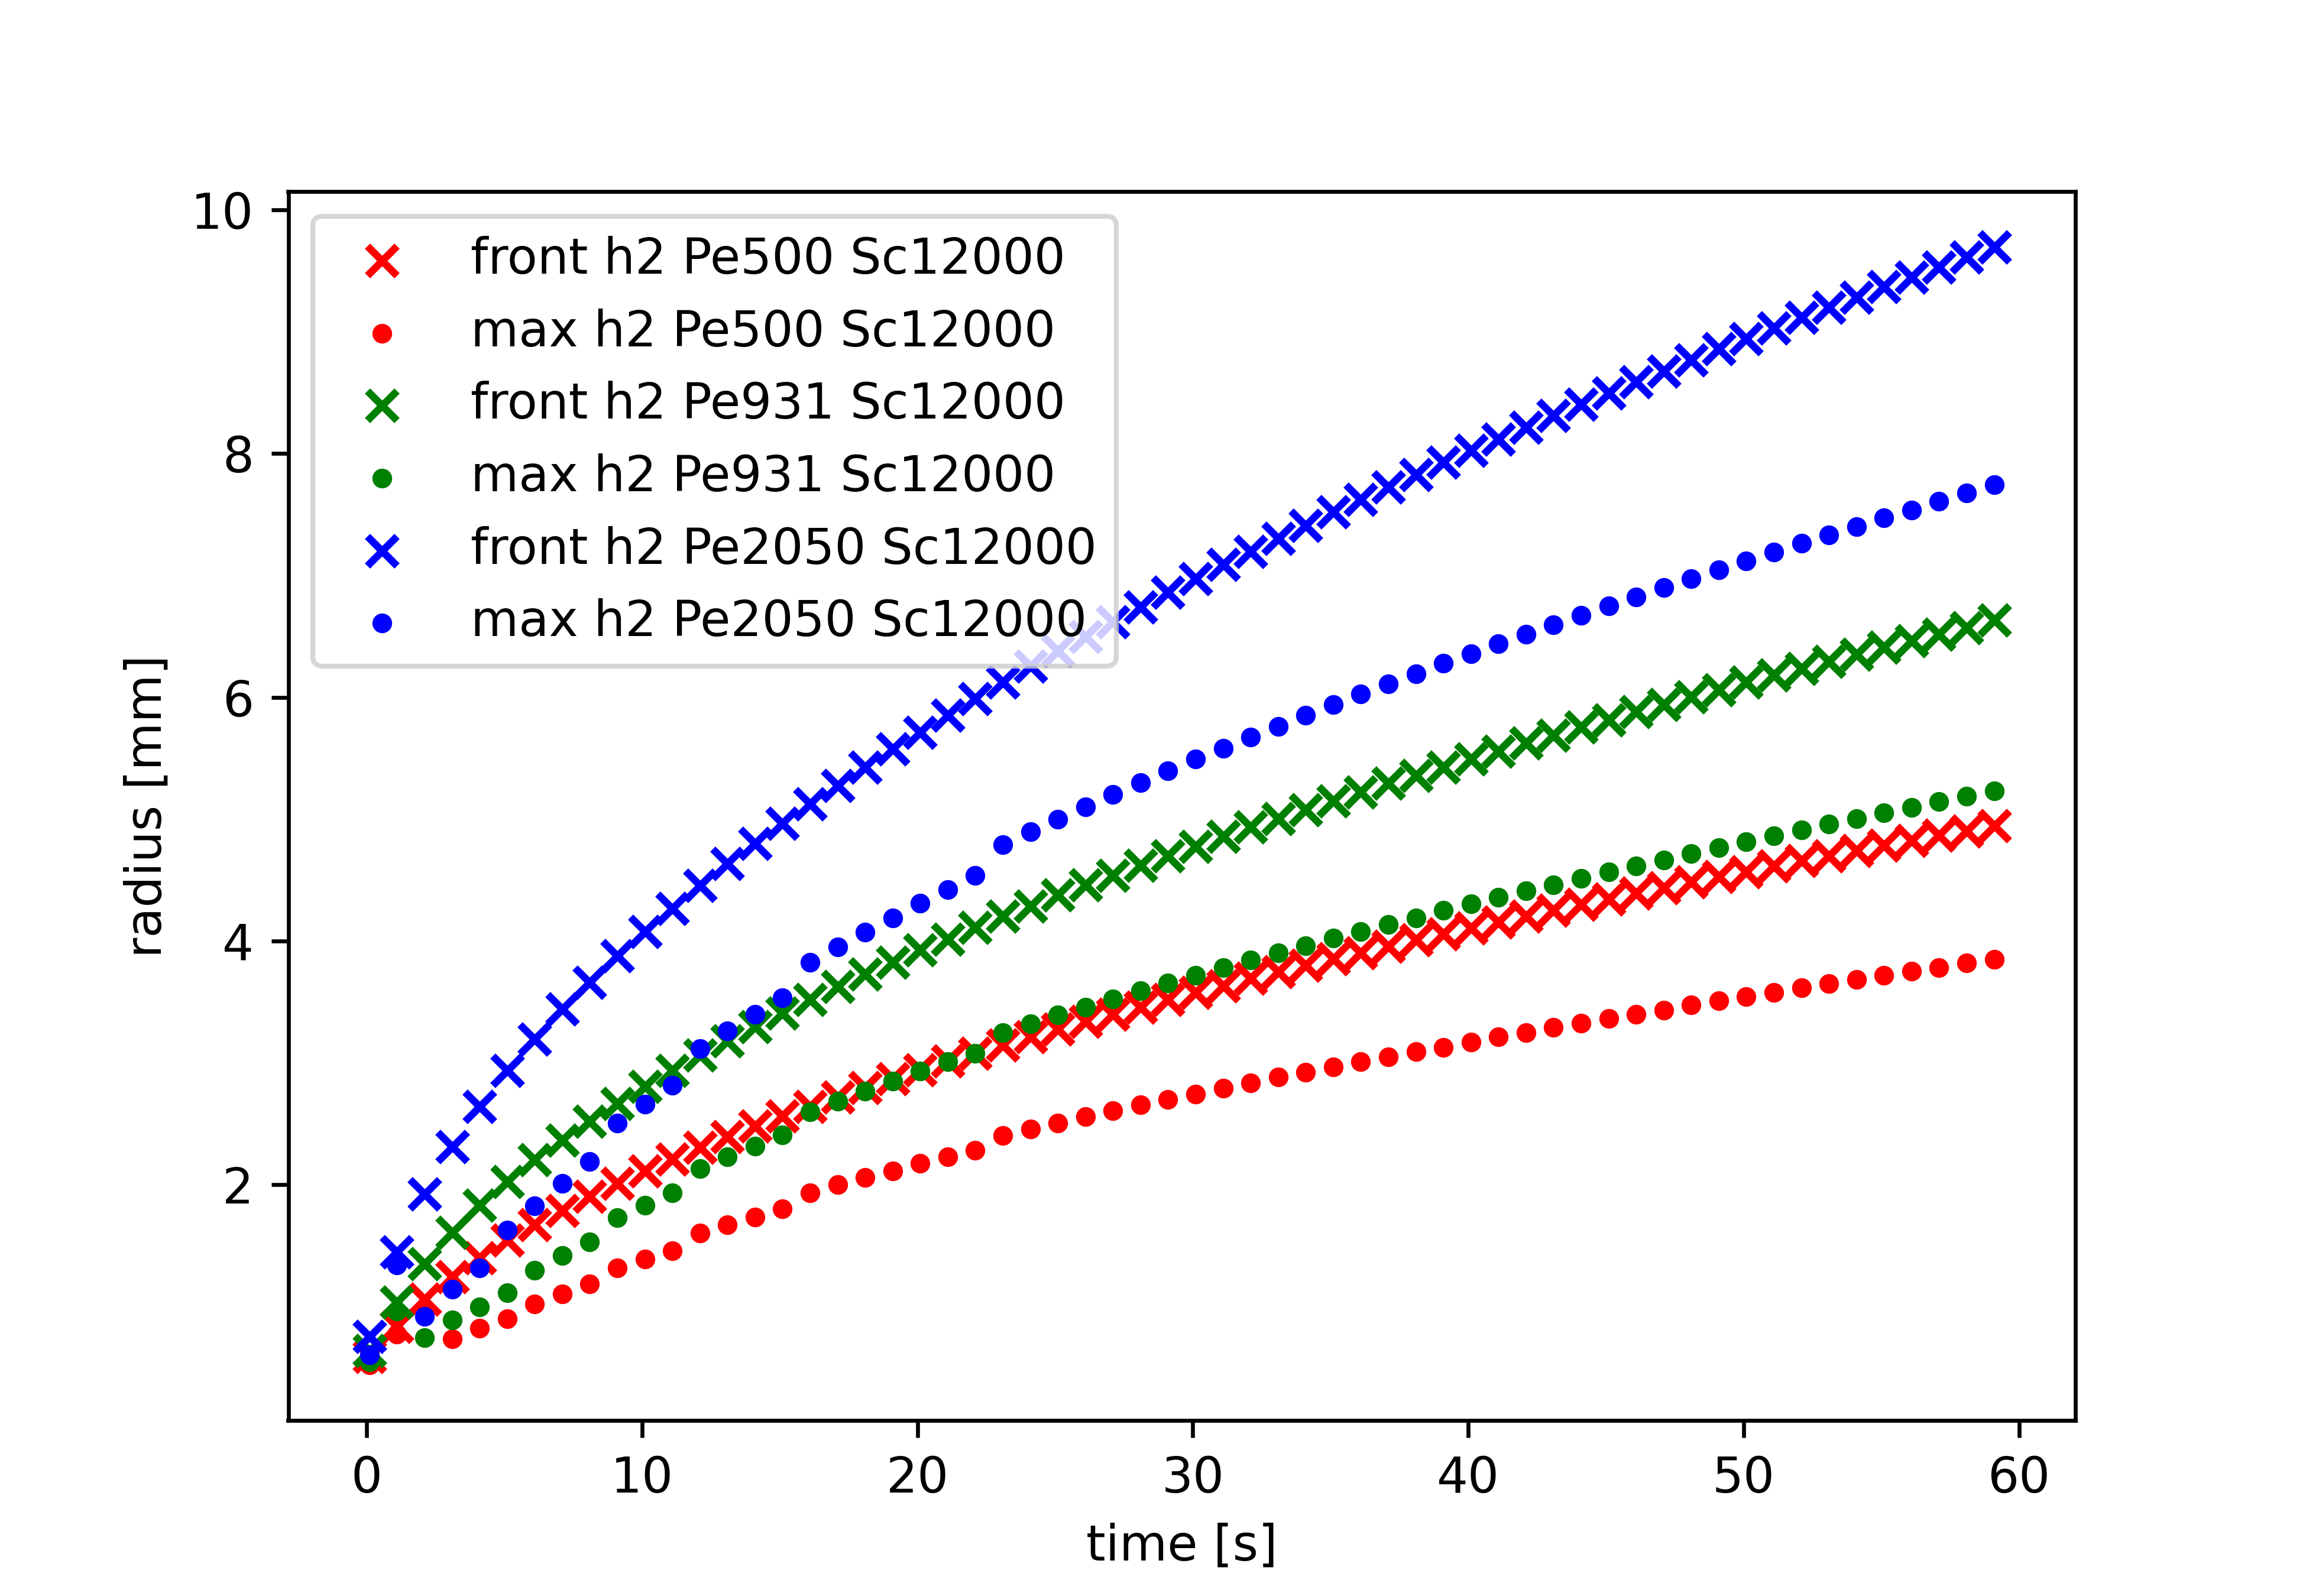
\includegraphics[width=.9\linewidth]{front_pos_h2_Sc12000}
	\caption{Front positions for  h = 0.2mm Sc = 12000
	\label{fig: front_pos_h2_Sc12000}}
\end{figure}
For a Schmidt number of 12000 the values for $r_{\text{front}}$ and $r_{\text{max}}$ do show a similar behaviour on a principle level. The $r_{\text{front}}$ positions travel speed decays over time and seems to follow an approach close to a square root function. The values for $r_{\text{max}}$ do show the same behaviour, but are always at lower radial values than the front values $r_{\text{front}}$.
\begin{figure}[htb]
	\centering
	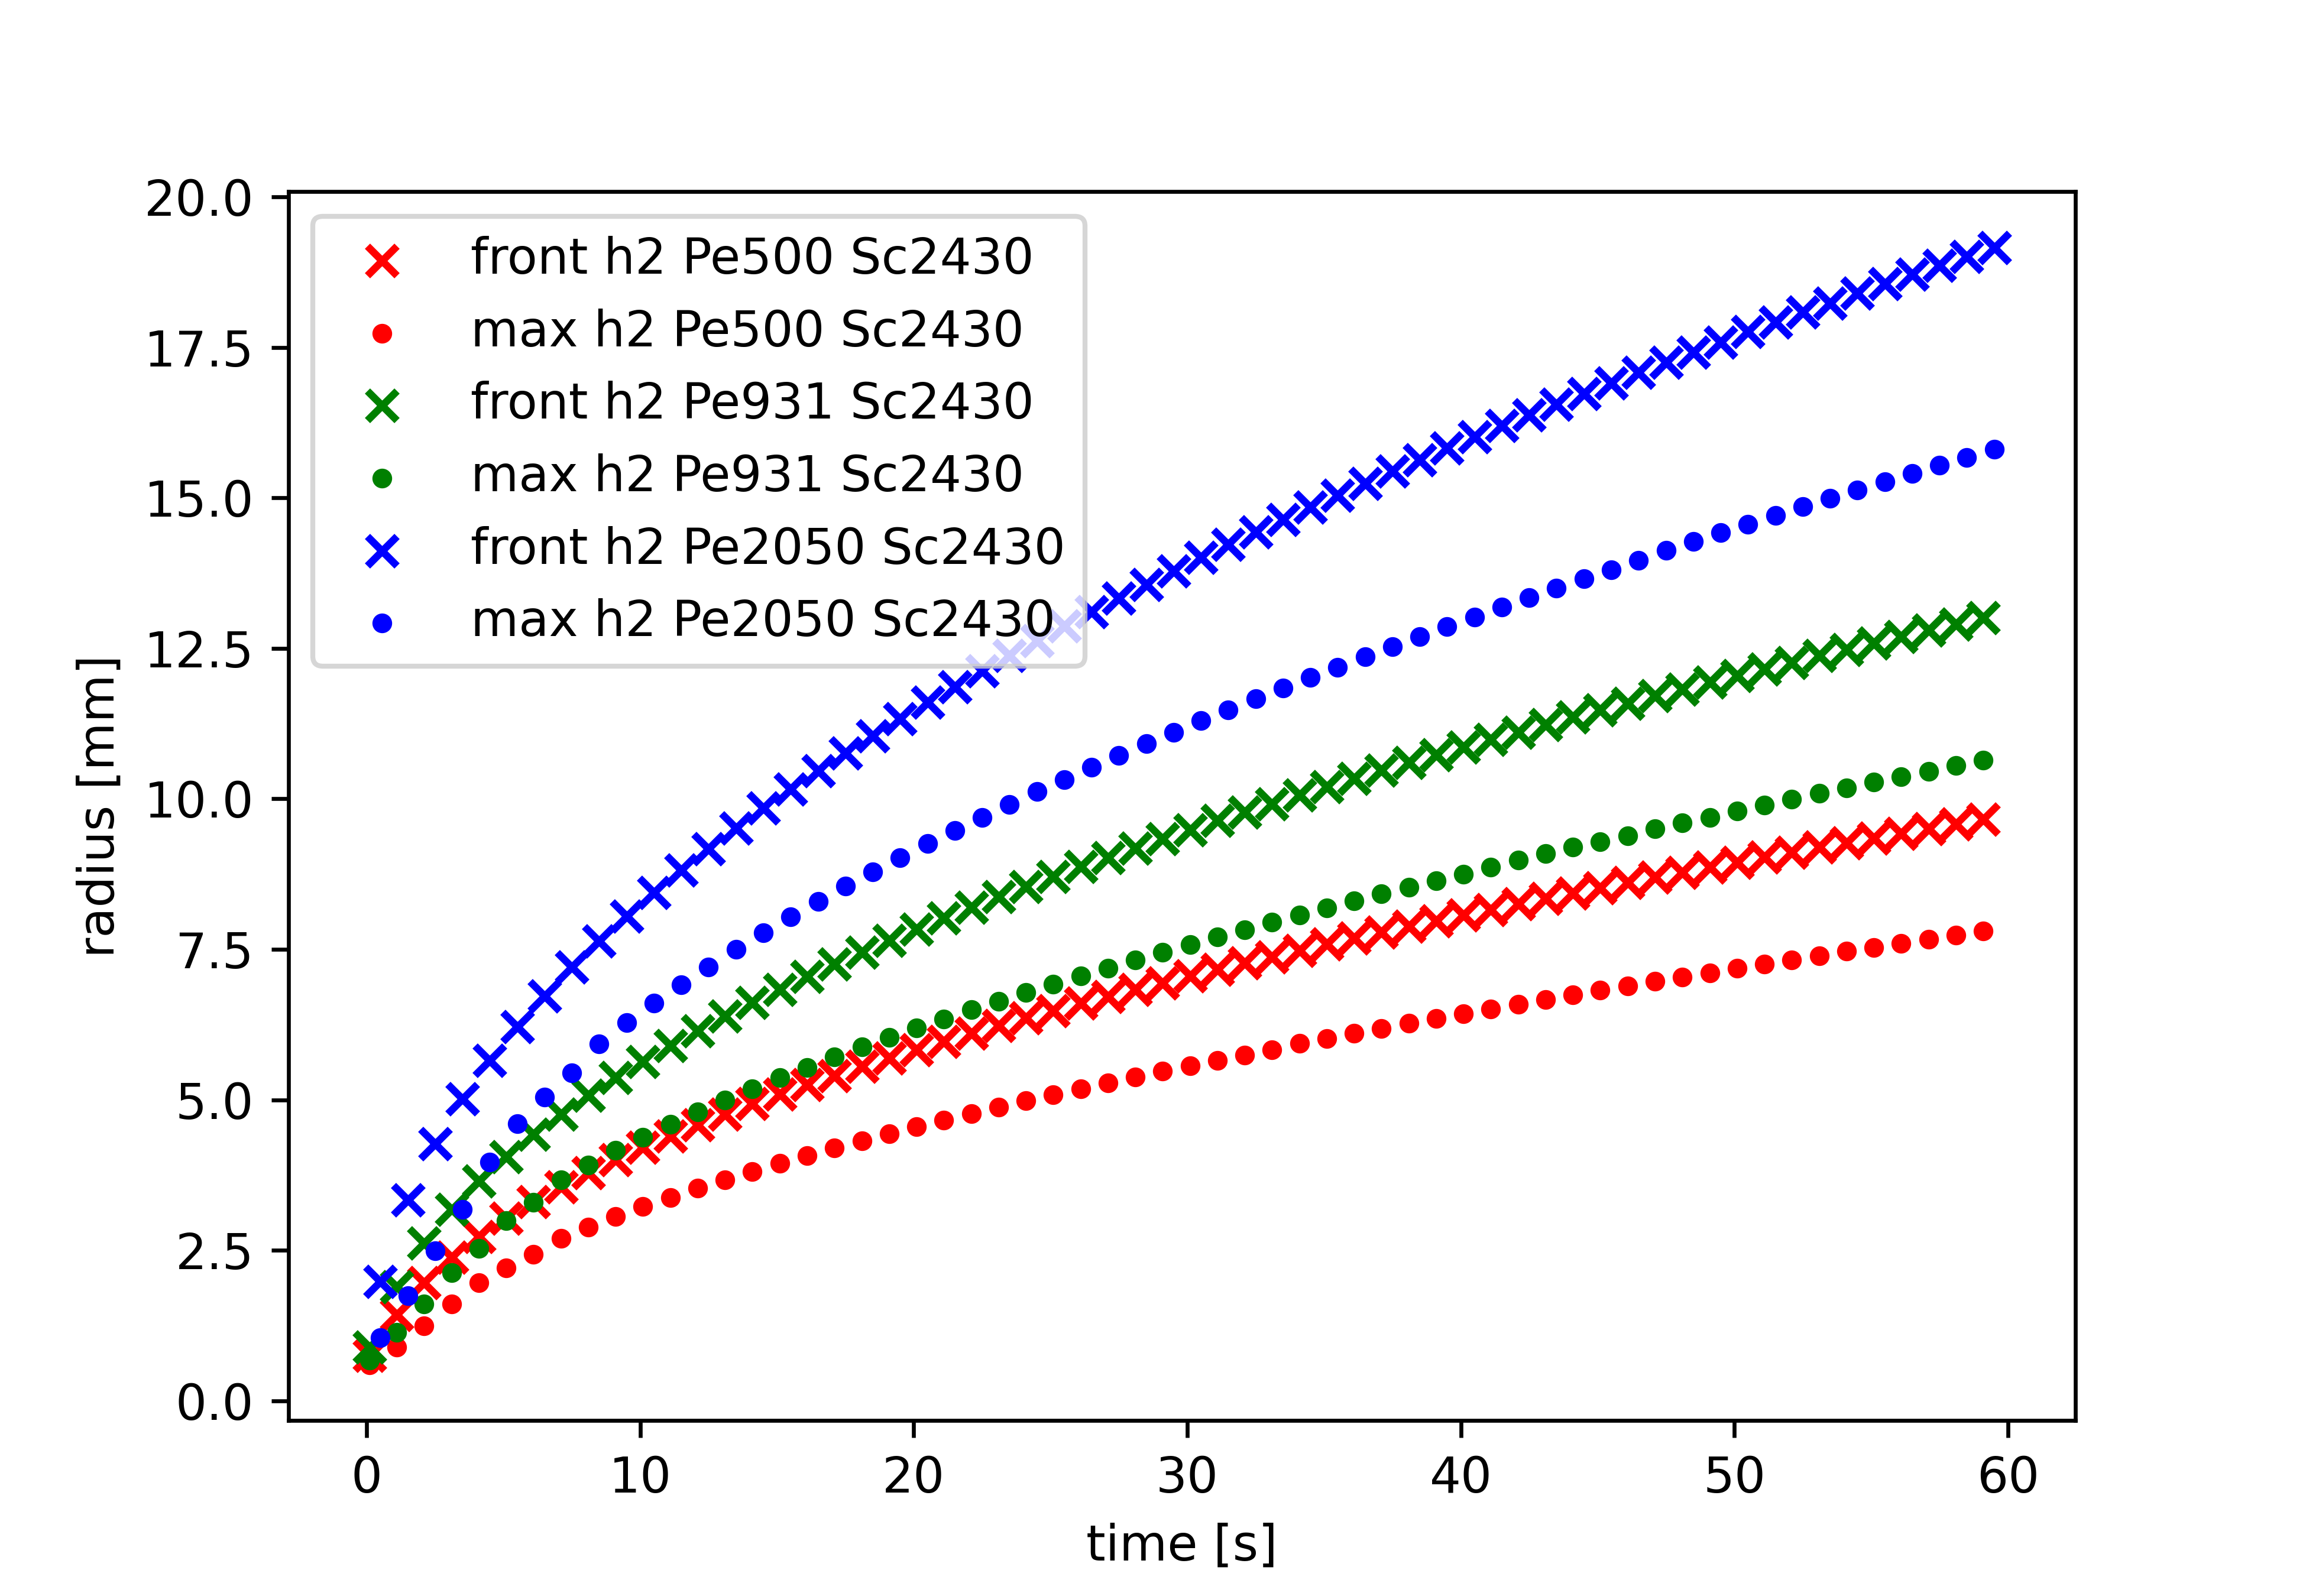
\includegraphics[width=.9\linewidth]{front_pos_h2_Sc2430}
	\caption{Front positions for  h = 0.2mm Sc = 2430
	\label{fig: front_pos_h2_Sc2430}}
\end{figure}

The described behaviour is the same for the cases with Sc = 2430.

The $r_{\text{front}}$ and $r_{\text{max}}$ positions travel faster for higher Peclet numbers, which can be explained by the different input velocities. With decreasing inlet velocity, the difference between the fronts front and maximum position at later time steps decreases. The decrease is more significant for cases with higher Peclet numbers. For cases with lower Peclet numbers the distance between  $r_{\text{front}}$ and $r_{\text{max}}$ at the end is approximately the same. This can be seen in \autoref{fig: front_pos_h2_Sc2430} when looking at the plots for Pe = 500 and comparing it with the ones for Pe = 931. For these cases, due to their lower absolute inlet velocity, the distance between the front's front and maximum is smaller and doesn't change that much if the velocity is risen or lowered.

When comparing the plots for Schmidt number 2430 with the one for a Schmidt number of 12000 it can be observed that all fronts travel nearly double the distance within the same time of 60 seconds. This can be explained mainly by the lower diffusion coefficient for the higher Schmidt number case. The diffusion coefficient for the lower Schmidt number case is $4 \text{.}11 \cdot 10^{-10} \left[ \frac{\mathrm{m^2}}{\mathrm{s}} \right]$ and the one for the higher Schmidt number case is $1\text{.}0 \cdot 10^{-10} \left[ \frac{\mathrm{m^2}}{\mathrm{s}} \right]$. In addition to the global Peclet number introduced in \autoref{eqn: Pe} a local one can be defined using \autoref{eqn: Pe local}.
\begin{equation}
	Pe_{\text{local}} = \dfrac{h \cdot u(x,r)}{D}
	\label{eqn: Pe local}
\end{equation}
In this equation the local velocity $u(x,r)$ at the coordinates $x$ and $r$ is used instead of the inlet velocity $u$ used within the global Peclet-Number.
Since the velocity magnitude decreases very quickly for a axisymmetric reactor (see \autoref{fig: field_example}) $Pe_{\text{local}}$ does show the same behaviour as they are directly linked to each other. As the Peclet number is defined as the advective transport rate divided by the diffusive transport rate, a low local Peclet number means that diffusion plays a more and more significant role while the front travels through the reactor. 

The diffusion coefficient has not only an influence on the front's position. The front's width is affected by diffusion as well. The fronts width will be analysed within the following section.

\section{Front Widths}

The fronts width behaviour is quite different for each reactor geometry, so each one will be looked at starting with the smallest gap height of 0.2mm. The front widths for that geometry are shown in \autoref{fig: front_width_h2_Sc12000} and \autoref{fig: front_width_pos_h2_Sc2430} for each investigated Schmidt number.
\begin{figure}[htbp]
	\centering
	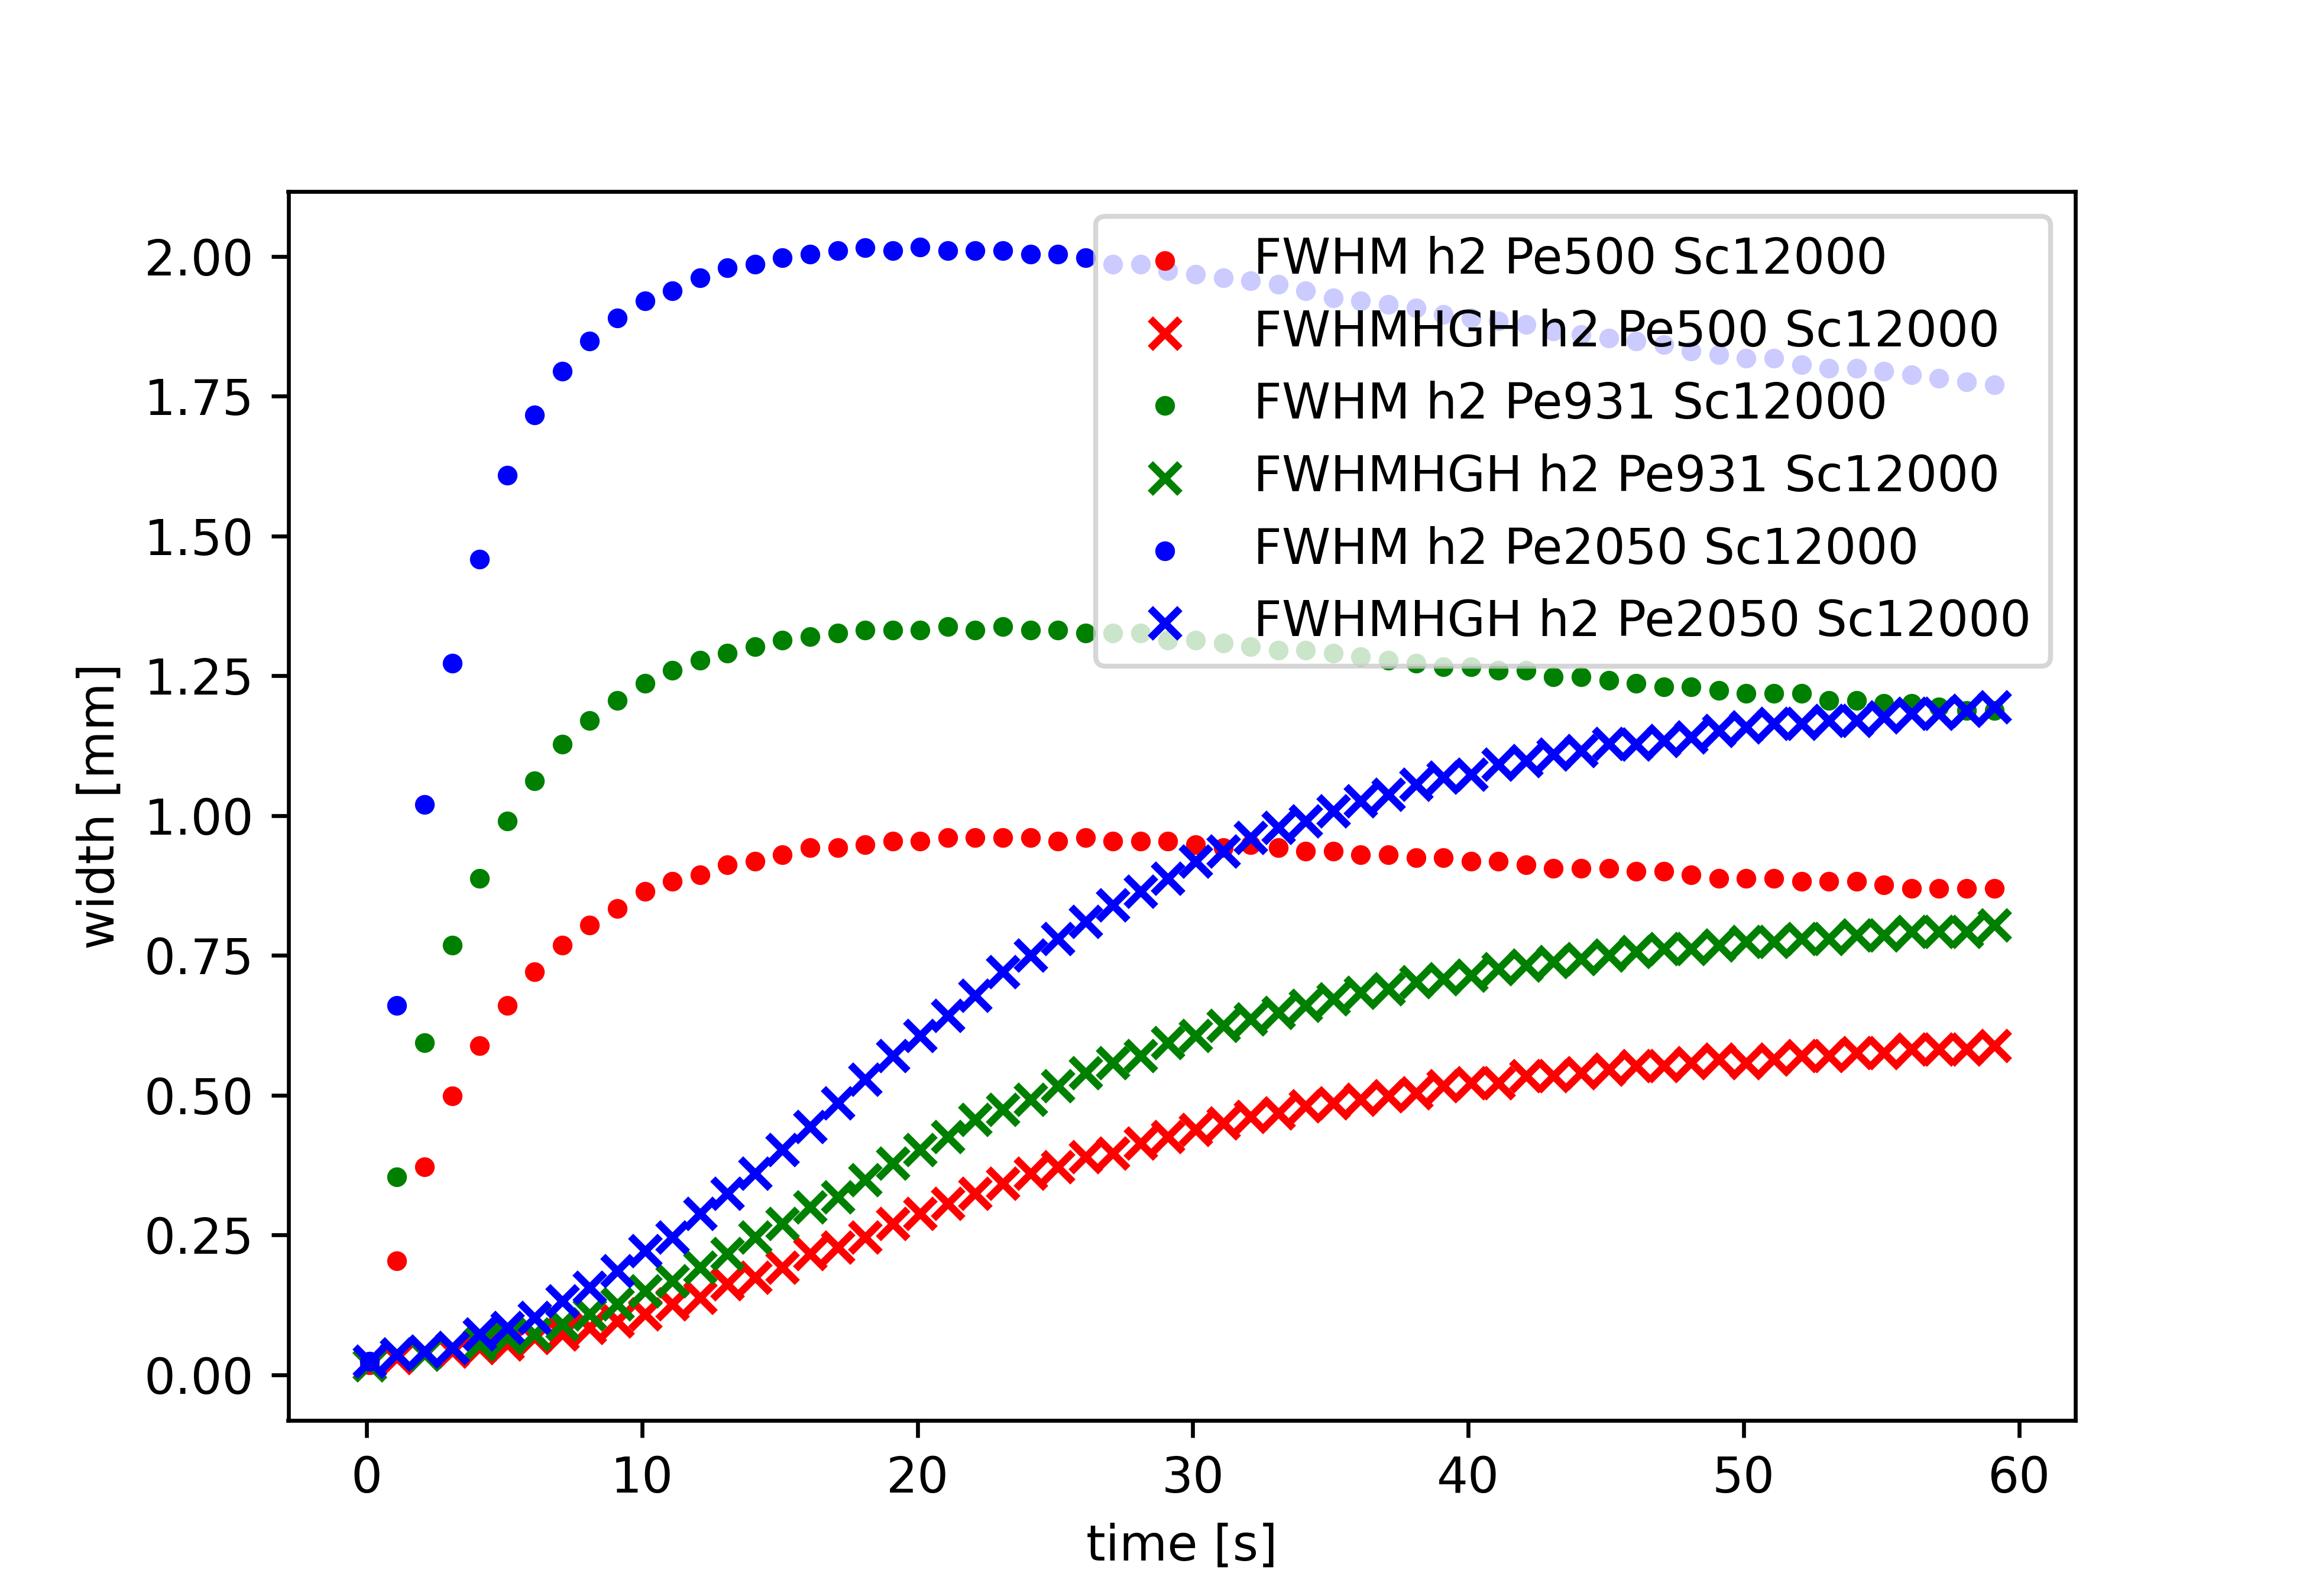
\includegraphics[width=0.8\linewidth]{front_width_h2_Sc12000}
	\caption{Front widths for  h = 0.2mm Sc = 12000
	\label{fig: front_width_h2_Sc12000}}
\end{figure}
Within the plot for the Schmidt number of 12000, it can be seen that the width using the gap averaged product concentration data (FWHM) starts growing fast within the first seconds. After that the widths growth slows down and the width reaches it's maximum value. When the maximum has been reached the width starts shrinking slowly towards a final constant value. The FWHMHGH does show a different behaviour. Its growth starts slow within the first few seconds and then starts to follow a square root like approach towards a final constant value. The widths do reach higher values for higher Peclet numbers.
\begin{figure}[htbp]
	\centering
	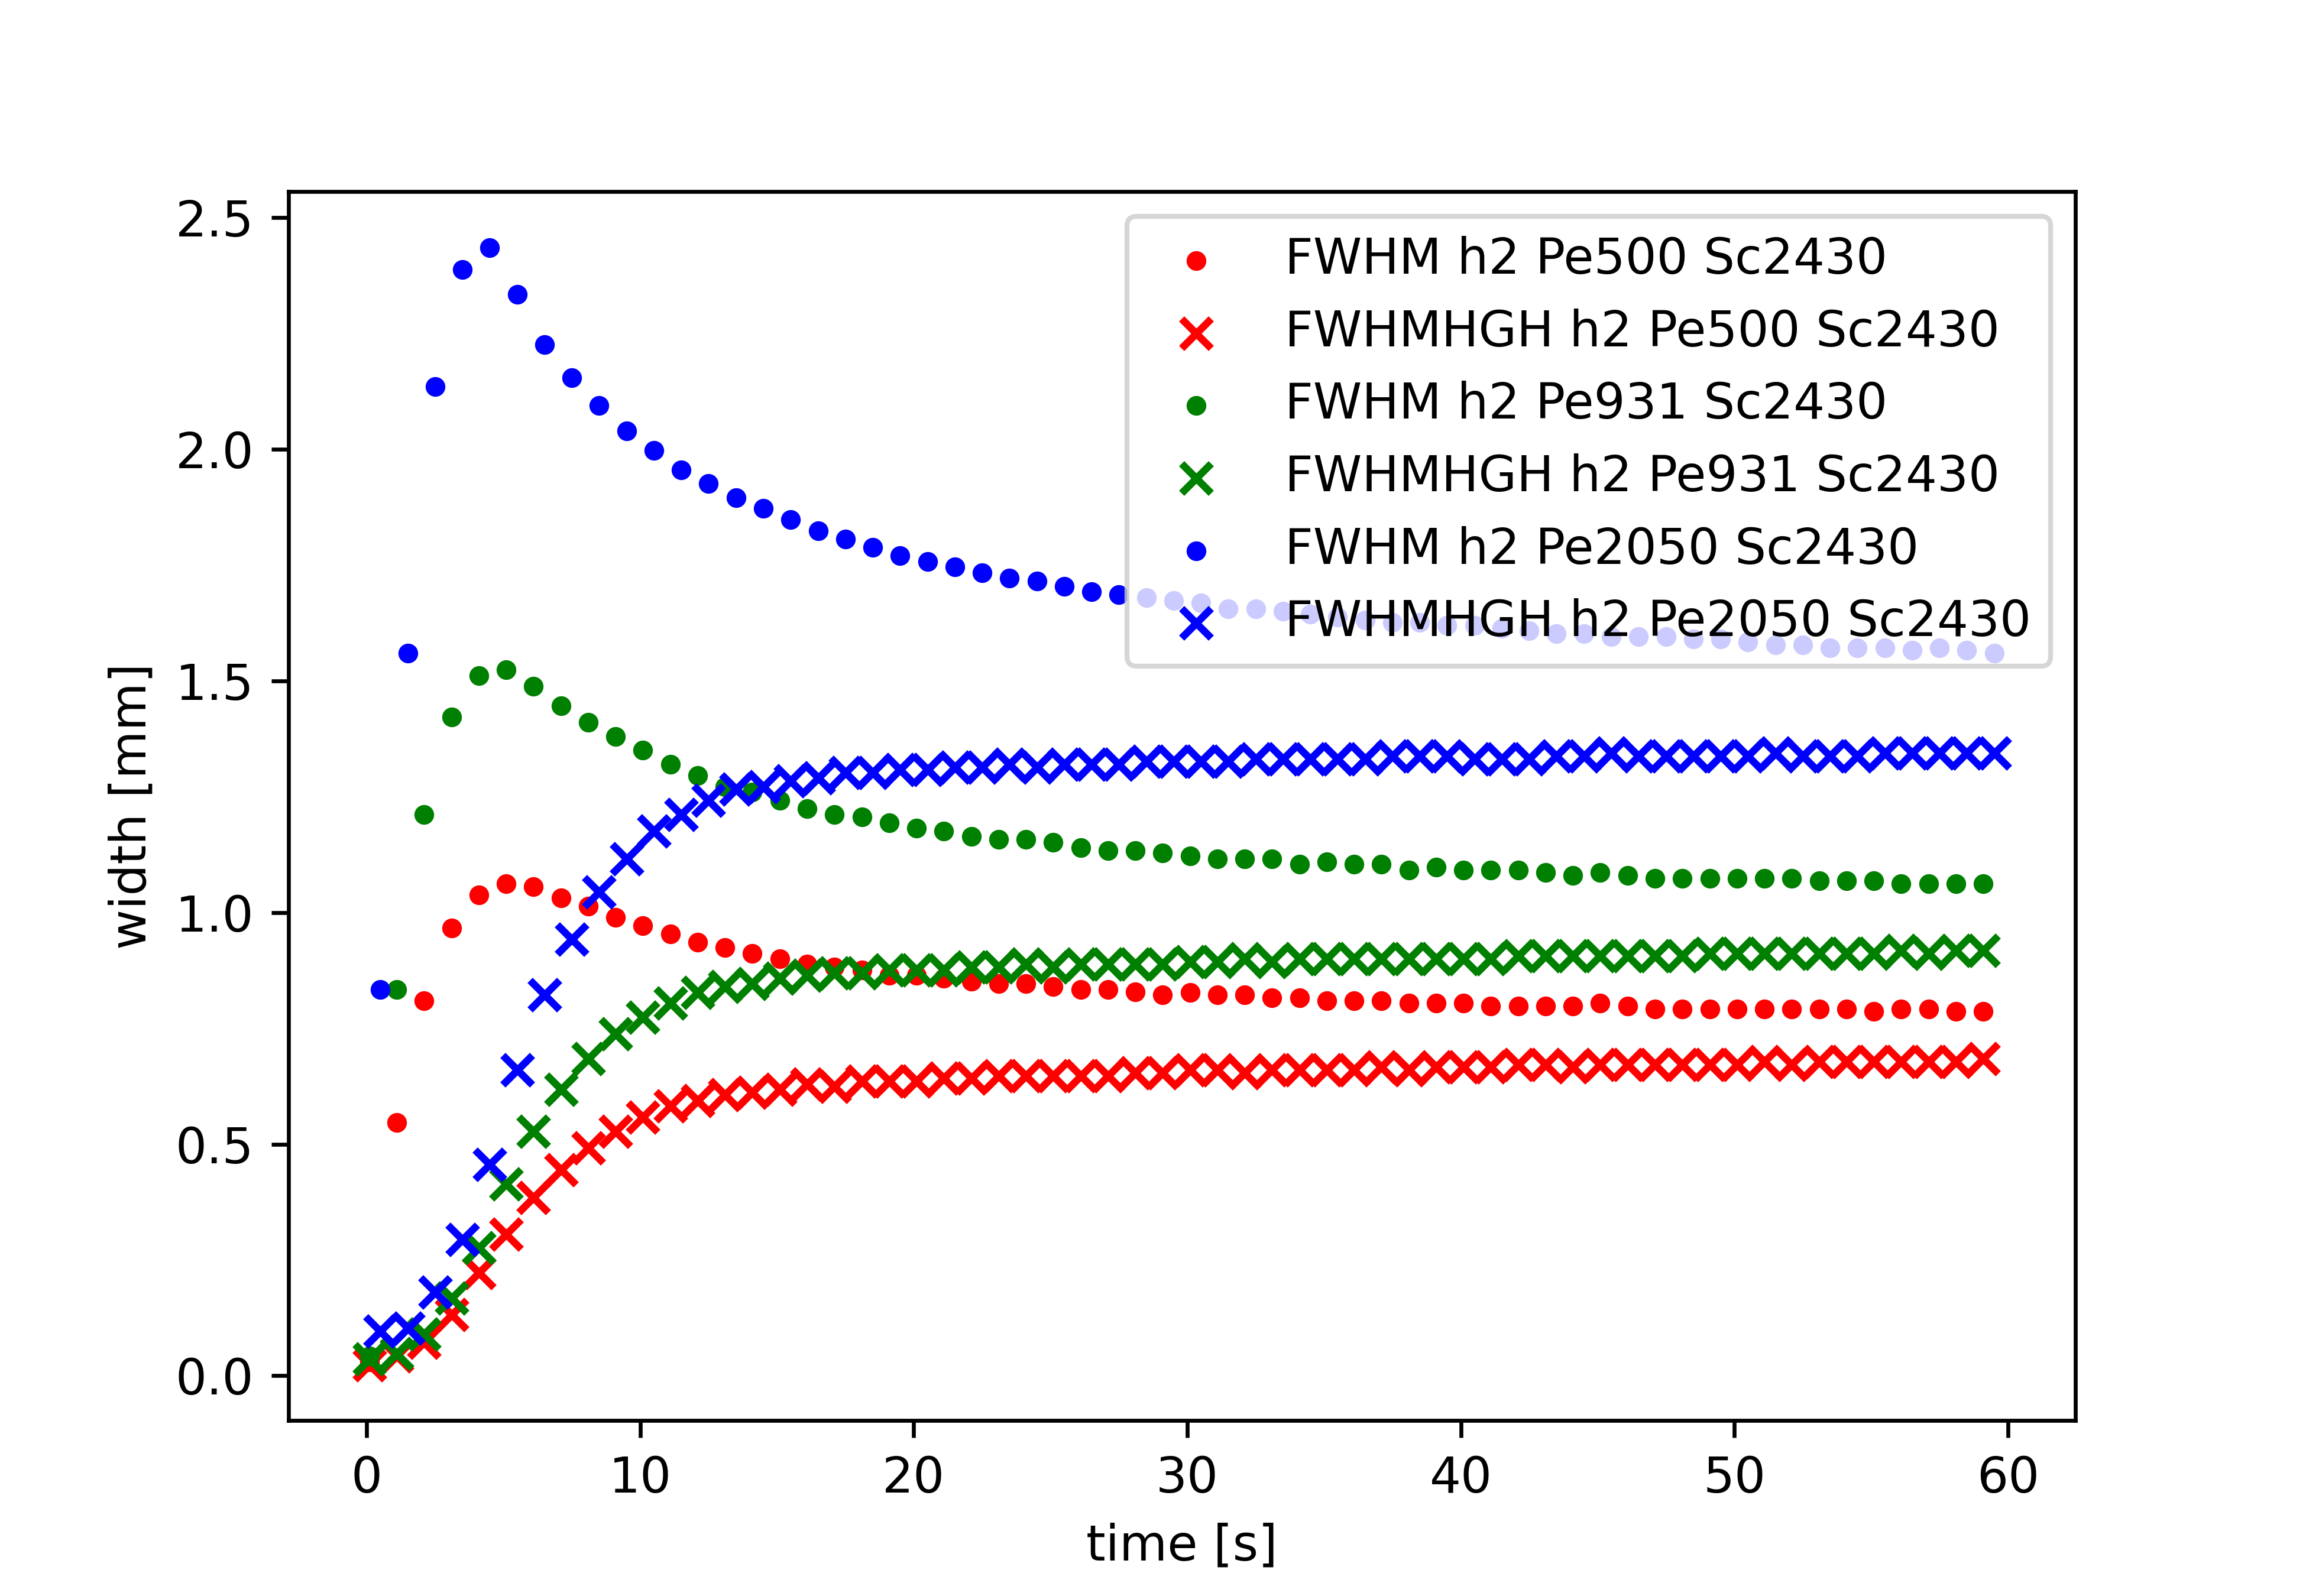
\includegraphics[width=0.8\linewidth]{front_width_h2_Sc2430}
	\caption{Front widths for  h = 0.2mm Sc = 2430}
	\label{fig: front_width_pos_h2_Sc2430}
\end{figure}
For the case with a Schmidt number of 2430 the width's growth in the beginning is even faster compared to the cases with the higher Schmidt number. This faster growth can be seen for both the FWHM as well as the FWHMHGH. The decrease after the front has reached it's maximum value is more visible for the lower Schmidt number cases. From these cases it can be seen that both calculated widths seem to be driven towards the same value for later times. The same behaviour is expected to happen at later times for the simulation in the cases with Sc = 12000, which no results are calculated for.

The reason for the initial high growth is, that the front is near the inlet and new reactants are constantly available due to the high flow rate in that region. In addition to that the front's width has low values so the distance both reactants $A$ and $B$ need to travel to reach each other to form the product $C$ is low. In the beginning the front's shape can be represented by a straight line, which gets distorted over time as visible in \autoref{fig: shape_examp}a. This distortion creates new surface area for the reaction to take place, in addition to the area generated by the front's travelling in a radial reactor.

The strive towards the same value for both the FWHM and the FWHMHGH at later times can be explained by the fronts shape. In \autoref{fig: pos_h2_late} the product concentration field is shown at the time of 60 seconds, for the case with a Peclet number of 500 and a Schmidt number of 2430.
\begin{figure}[htb]
	\centering
	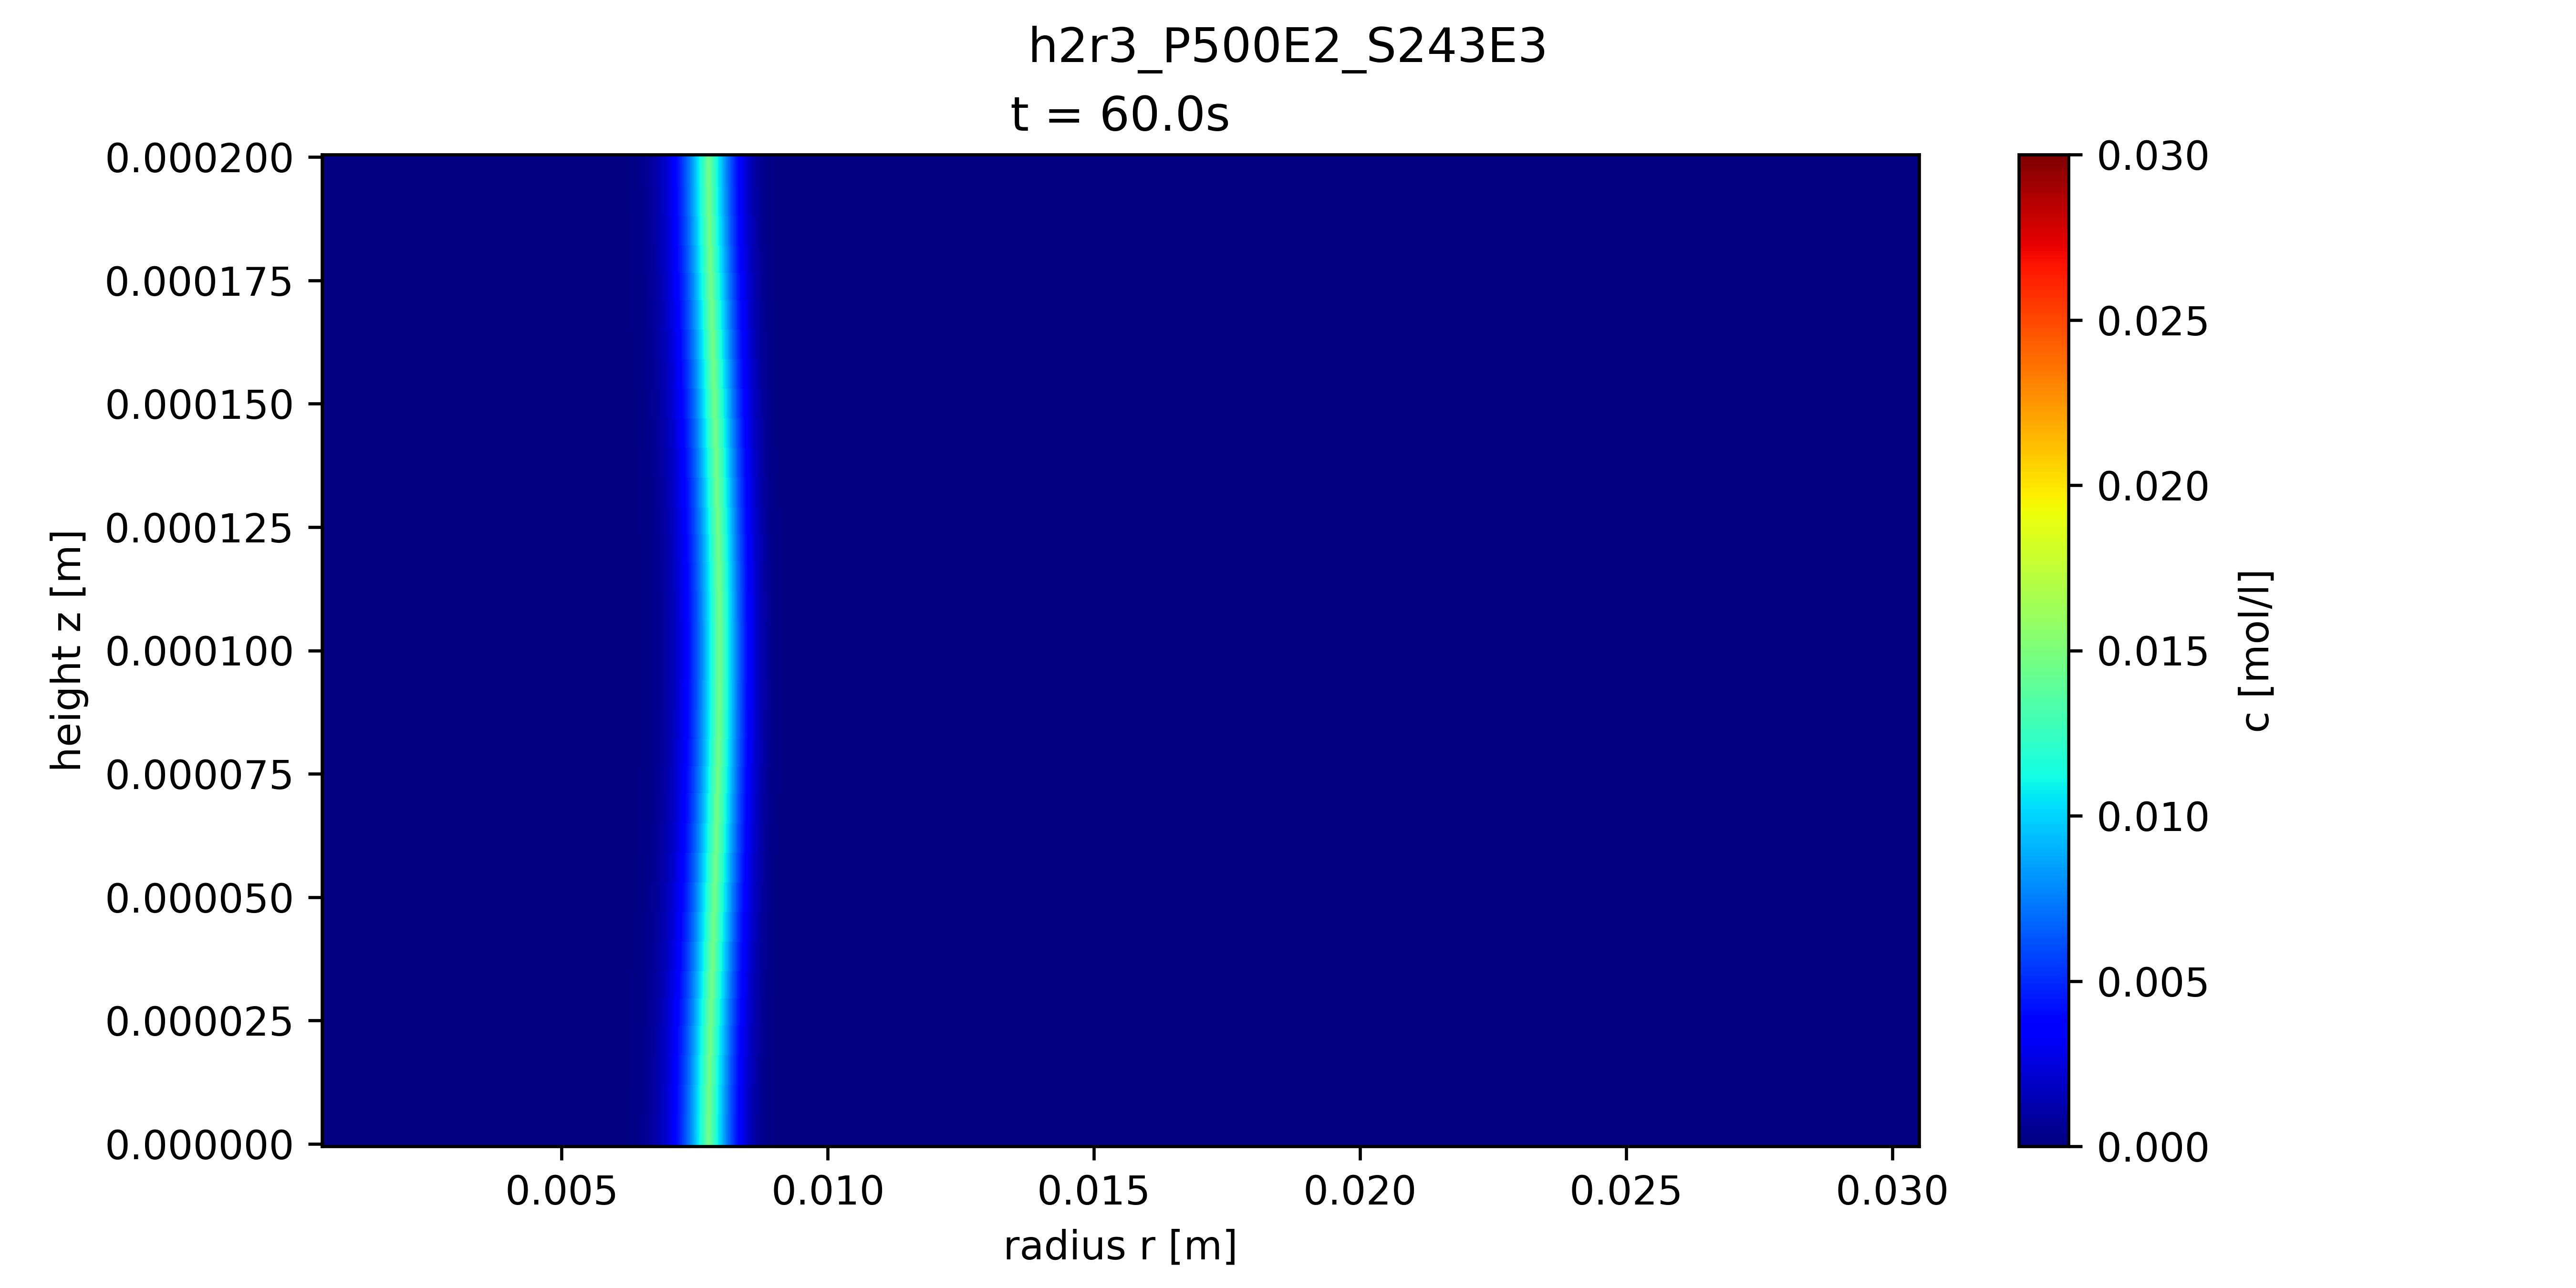
\includegraphics[width=\textwidth]{img_gif_h2r3_P500E2_S243E3_60,0 }
	\caption{Front shape for h=0.2mm Pe = 500 Sc = 2430 at 60 seconds}
	\label{fig: pos_h2_late}
\end{figure}
When the front reaches the shown shape, the difference between the width using the FWHM method and the middle with decreases. As shown in \cite{comolli2021dynamics}, the reaction decays until the spreading of front by diffusion forms an equilibrium with the reactants consumed by the reaction.

Another reason for the decay could be that the maximum value changes, so the positions the widths are taken from do change as well. In \autoref{fig: plot_h2_widths} the gap averaged concentration plots are shown for a time of 2 seconds which is in the phase of width growth, a time of 5 seconds which is close to the maximum and a time of 18 seconds which is near the end of the decaying phase. From this plot it can be seen, that the curvature does change over time. It widens at first when comparing the curves for $t = 2s$ with $t = 5s$ and then narrows down. In addition to that the maximum value raises, since more product is generated over time. With the maximum value raising, the position of $0\text{.}5 \cdot c_{C,max}$ changes as well towards the more narrow section of the curve. 
\begin{figure}
	\centering
	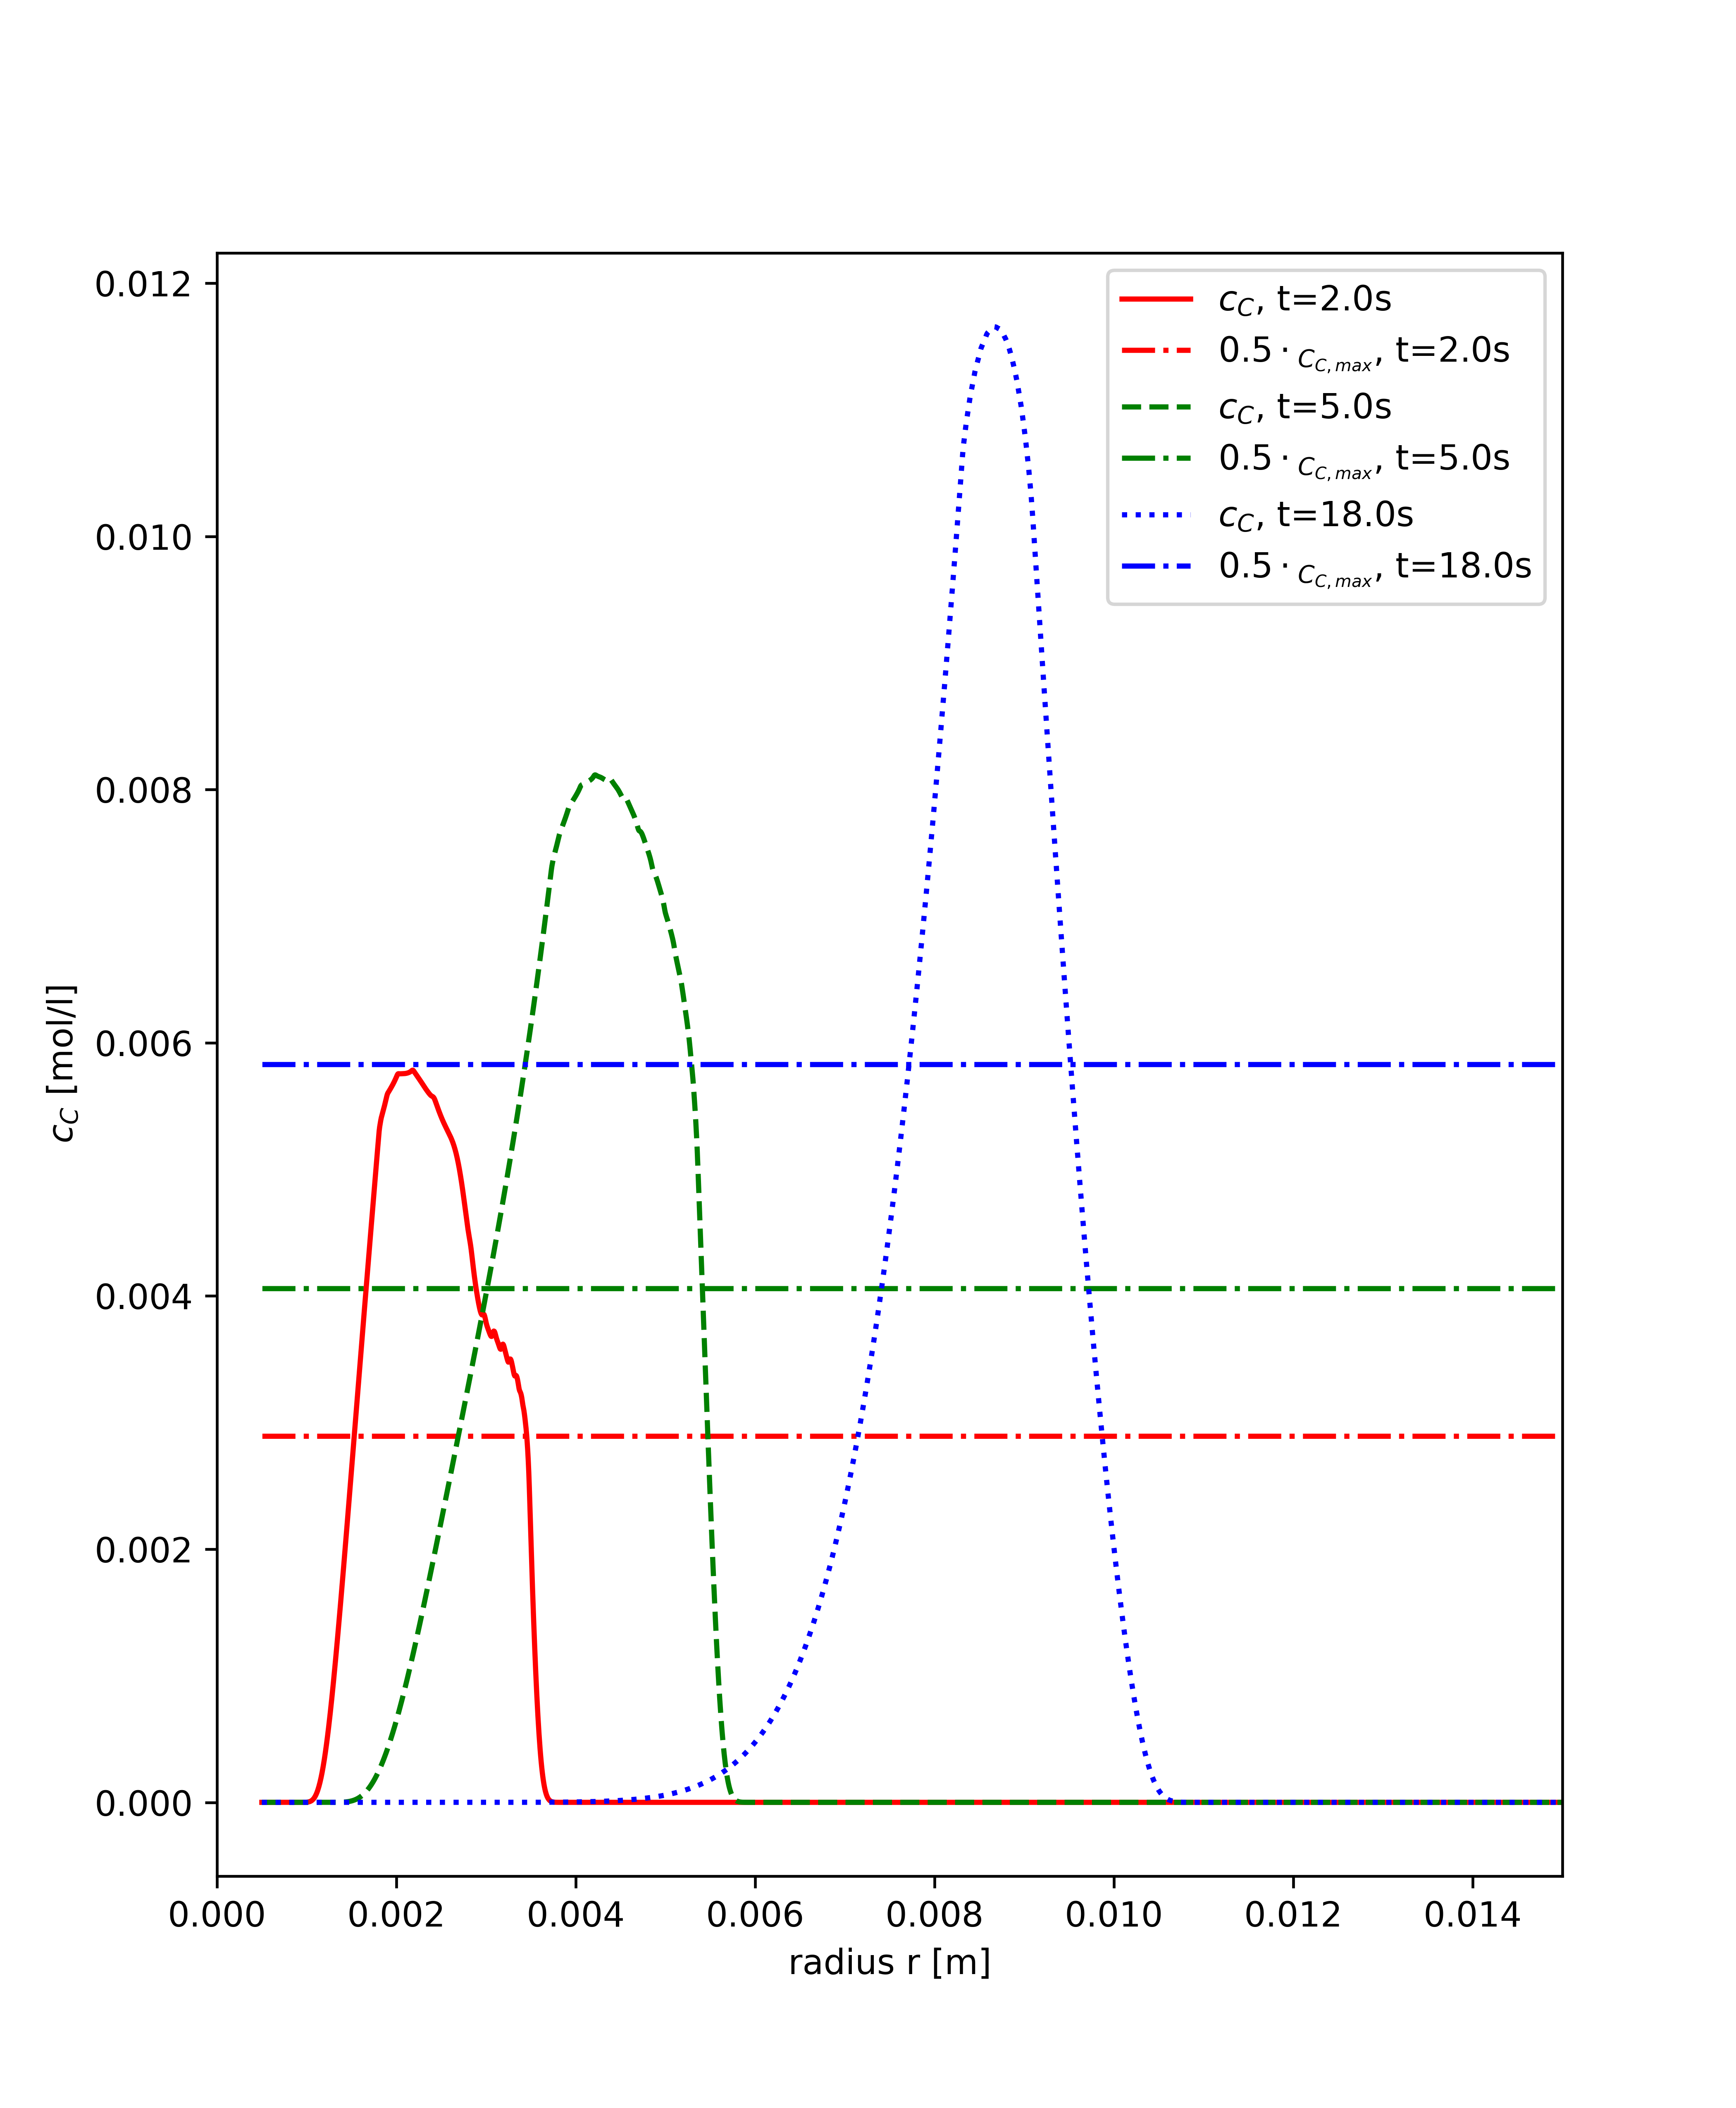
\includegraphics[width=\textwidth]{plot_h2r3_P205E3_S243E3_concentration-fluid_c}
	\caption{Product concentration plots for h = 0.2mm  Pe = 2050 Sc = 2430 for different times}
	\label{fig: plot_h2_widths}
\end{figure}

When comparing both Schmidt number plots with each other, it can be observed that the final width's value seems to be independent of the Schmidt number for a gap height of 0.2mm. For this gap height that is true for both the FWHM and the  FWHMHGH. The results from the 0.4mm case also support this assumption for the FWHM. To get clearer evidence if the assumption is correct, more Schmidt numbers need to be investigated and the simulations should be run for longer durations. These longer durations are also needed to get a clearer picture on how the FWHMHGH behaves at later stages of the simulation run.

Another observation that can be made, is that the time the width reaches its maximum value and the maximum value itself is strongly influenced by the Schmidt number. For the lower Schmidt number of 2430 a clear peak is visible for all Peclet numbers. This forming peak seems to be expected, because the diffusion coefficient for the case with the higher Schmidt number of 12000 is lower than the one for the lower Schmidt number of 2430. A lower diffusion coefficient prevents the front from spreading so the width reaches higher values.
\newline

The results for the cases with a gap height of 0.4mm show in most parts a similar behaviour compared to the case with a gap height of 0.2mm.
\begin{figure}[htb]
	\centering
	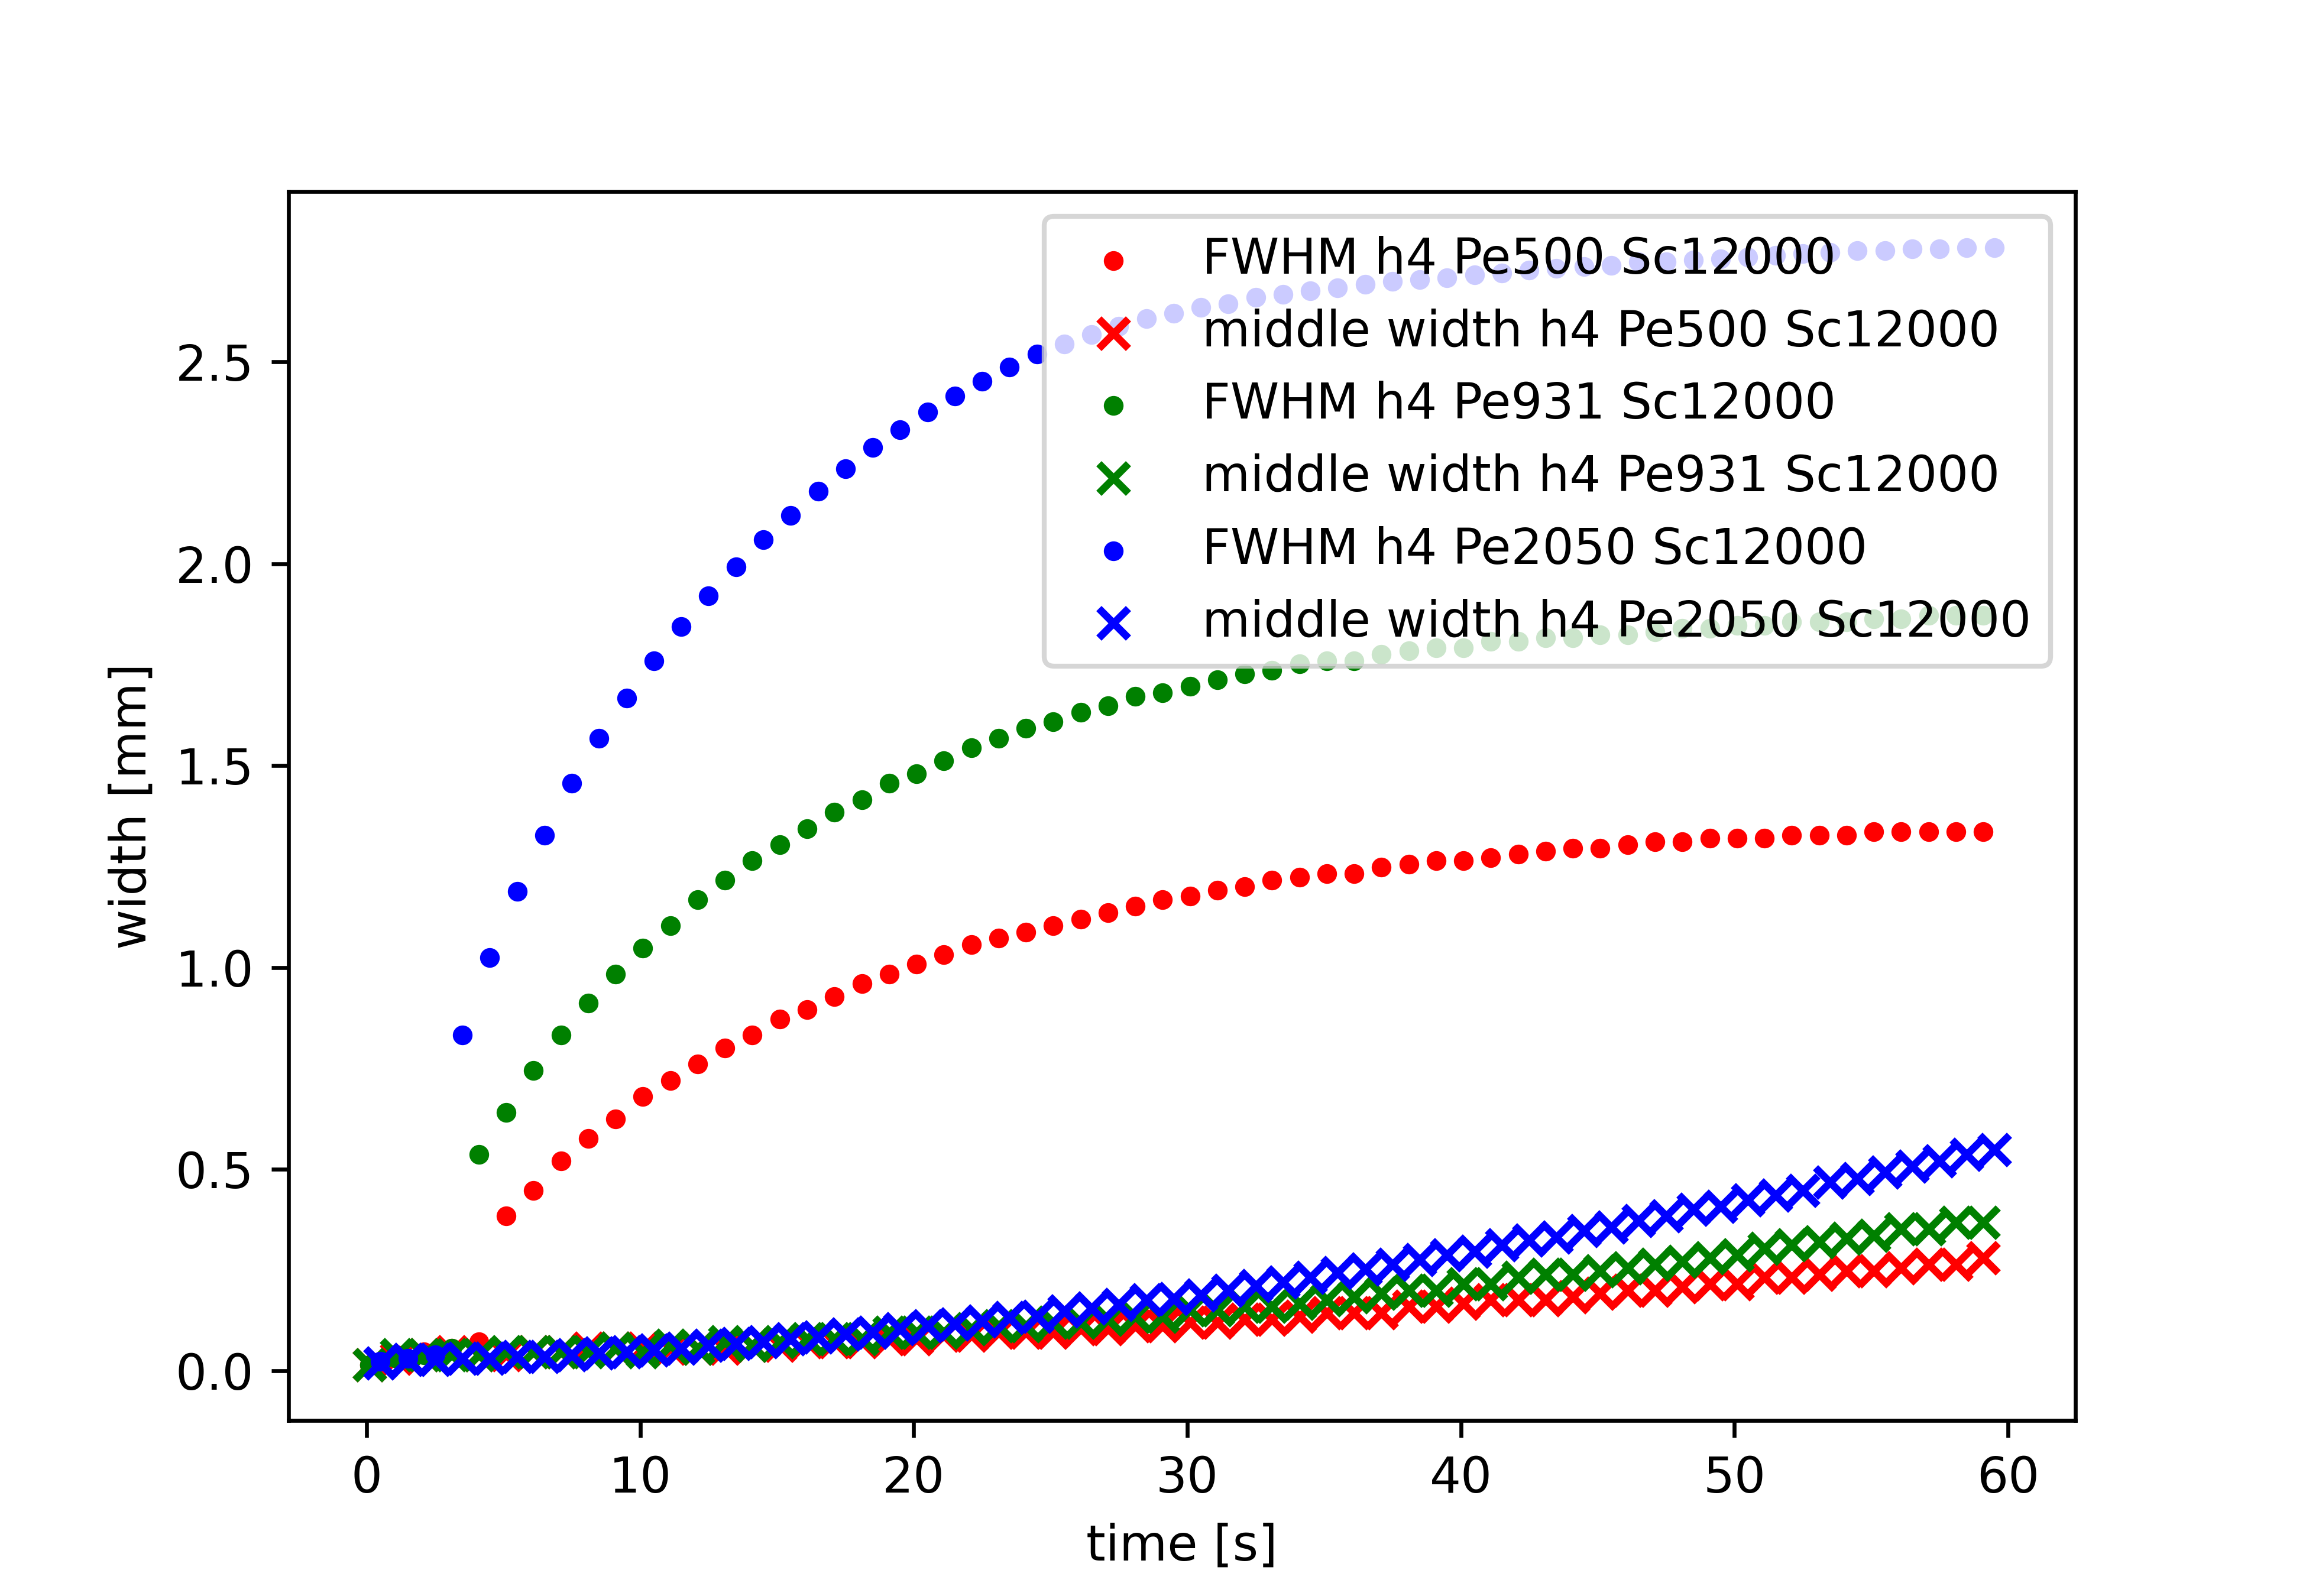
\includegraphics[width=0.85\textwidth]{front_width_h4_Sc12000}
	\caption{Front widths for  h = 0.4mm Sc = 12000
	\label{fig: front_width_h4_Sc12000}}
\end{figure}
For the case with the higher Schmidt number of 12000 the FWHM follows a square root like approach for all Peclet numbers. For the first 3 to 5 seconds the FWHM has very low values then starts to grow suddenly. The time the growth starts to happen is higher for lower Peclet numbers. The FWHMHGH has very low values over the hole simulation time for all Peclet numbers investigated. This width's growth seems to slightly increase at later times of around 40 seconds.
\begin{figure}[htb]
	\centering
	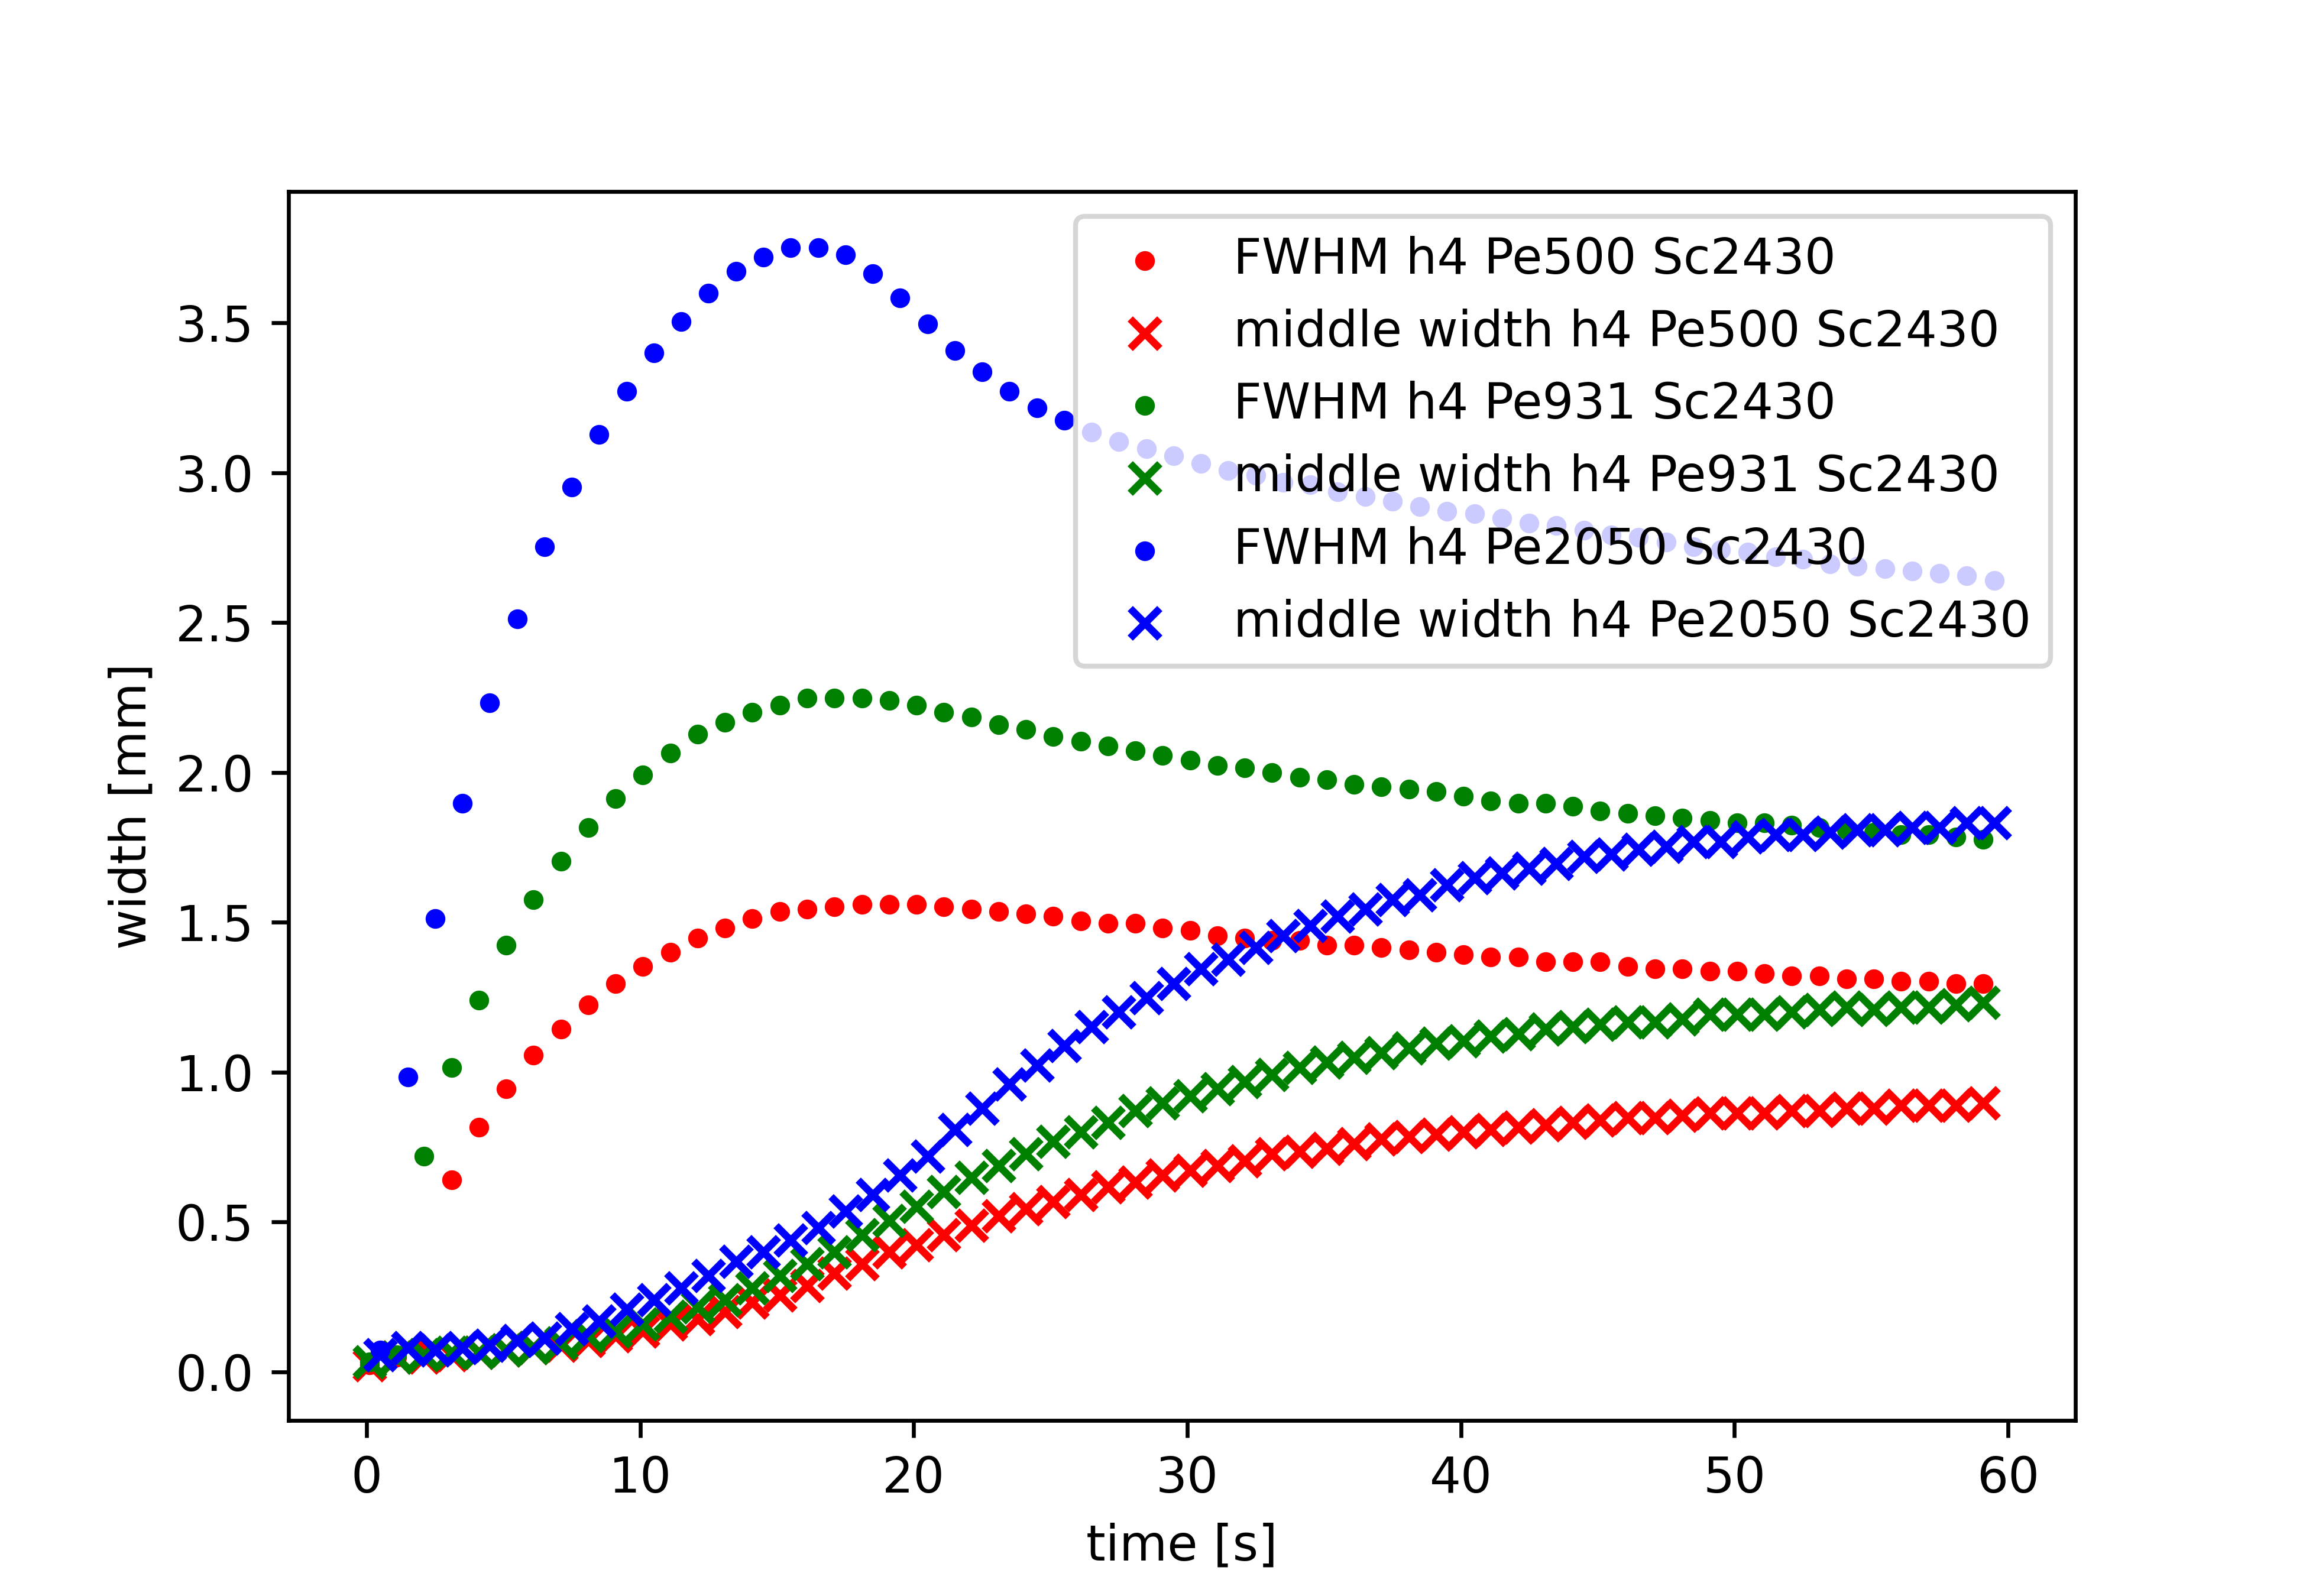
\includegraphics[width=.85\textwidth]{front_width_h4_Sc2430}
	\caption{Front widths for  h = 0.4mm Sc = 2430
		\label{fig: front_width_pos_h4_Sc2430}}
\end{figure}

The cases with the lower Schmidt number do show a comparable behaviour to the one for the height of 0.2mm, that do have the same Schmidt number. The FWHM curves show peaks as well but they are not that sharp and narrow compared against the ones in \autoref{fig: front_width_pos_h2_Sc2430}. The FWHMHGH behaves similar to the one with the same conditions at 0.2mm gap height, but the phase of growth is way longer and the constant value is reached near the end ot the 60 second simulation run time.

The square root like behaviour of the higher Schmidt number case can be explained by the fact, that the front is still in the phase of growing. This is comparable to the 0.2mm gap height cases for a time range of up to 20 seconds. For later times the FWHM is expected to decay as well as can be seen for the 0.2mm cases. The sudden growth is even more clearly visible for the gap height of 0.6mm and therefore explained there. The low growth rate of the FWHMHGH is the result of the high local Peclet number during most of the part of the simulation. The diffusive part only starts affecting this width at later times where the advective part loses it's influence on the front.

For the cases with the Schmidt number of 2430 the FWHM seems to reach it's highest value in the moment when the initial two different peaks visible within the concentration plots merge into one, which can be seen in \autoref{fig: pos_h4_peak_plots}. Up to a time of around 18 seconds two peaks can be distinguished within the product concentration plots. These two peaks are visible within the concentration plots, because the local Peclet number has lower values in the areas close to the walls. As a result of that, diffusion becomes more dominant in these regions, even at early times. This is clearly visible when looking at the product's concentration field at a times of 2 and 10 seconds in \autoref{fig: pos_h4_peak_fields}. The gap averaging operation then produces a large value in the front and back, that can be seen for the time of 2 seconds.

\begin{figure}[htbp]
	\centering
	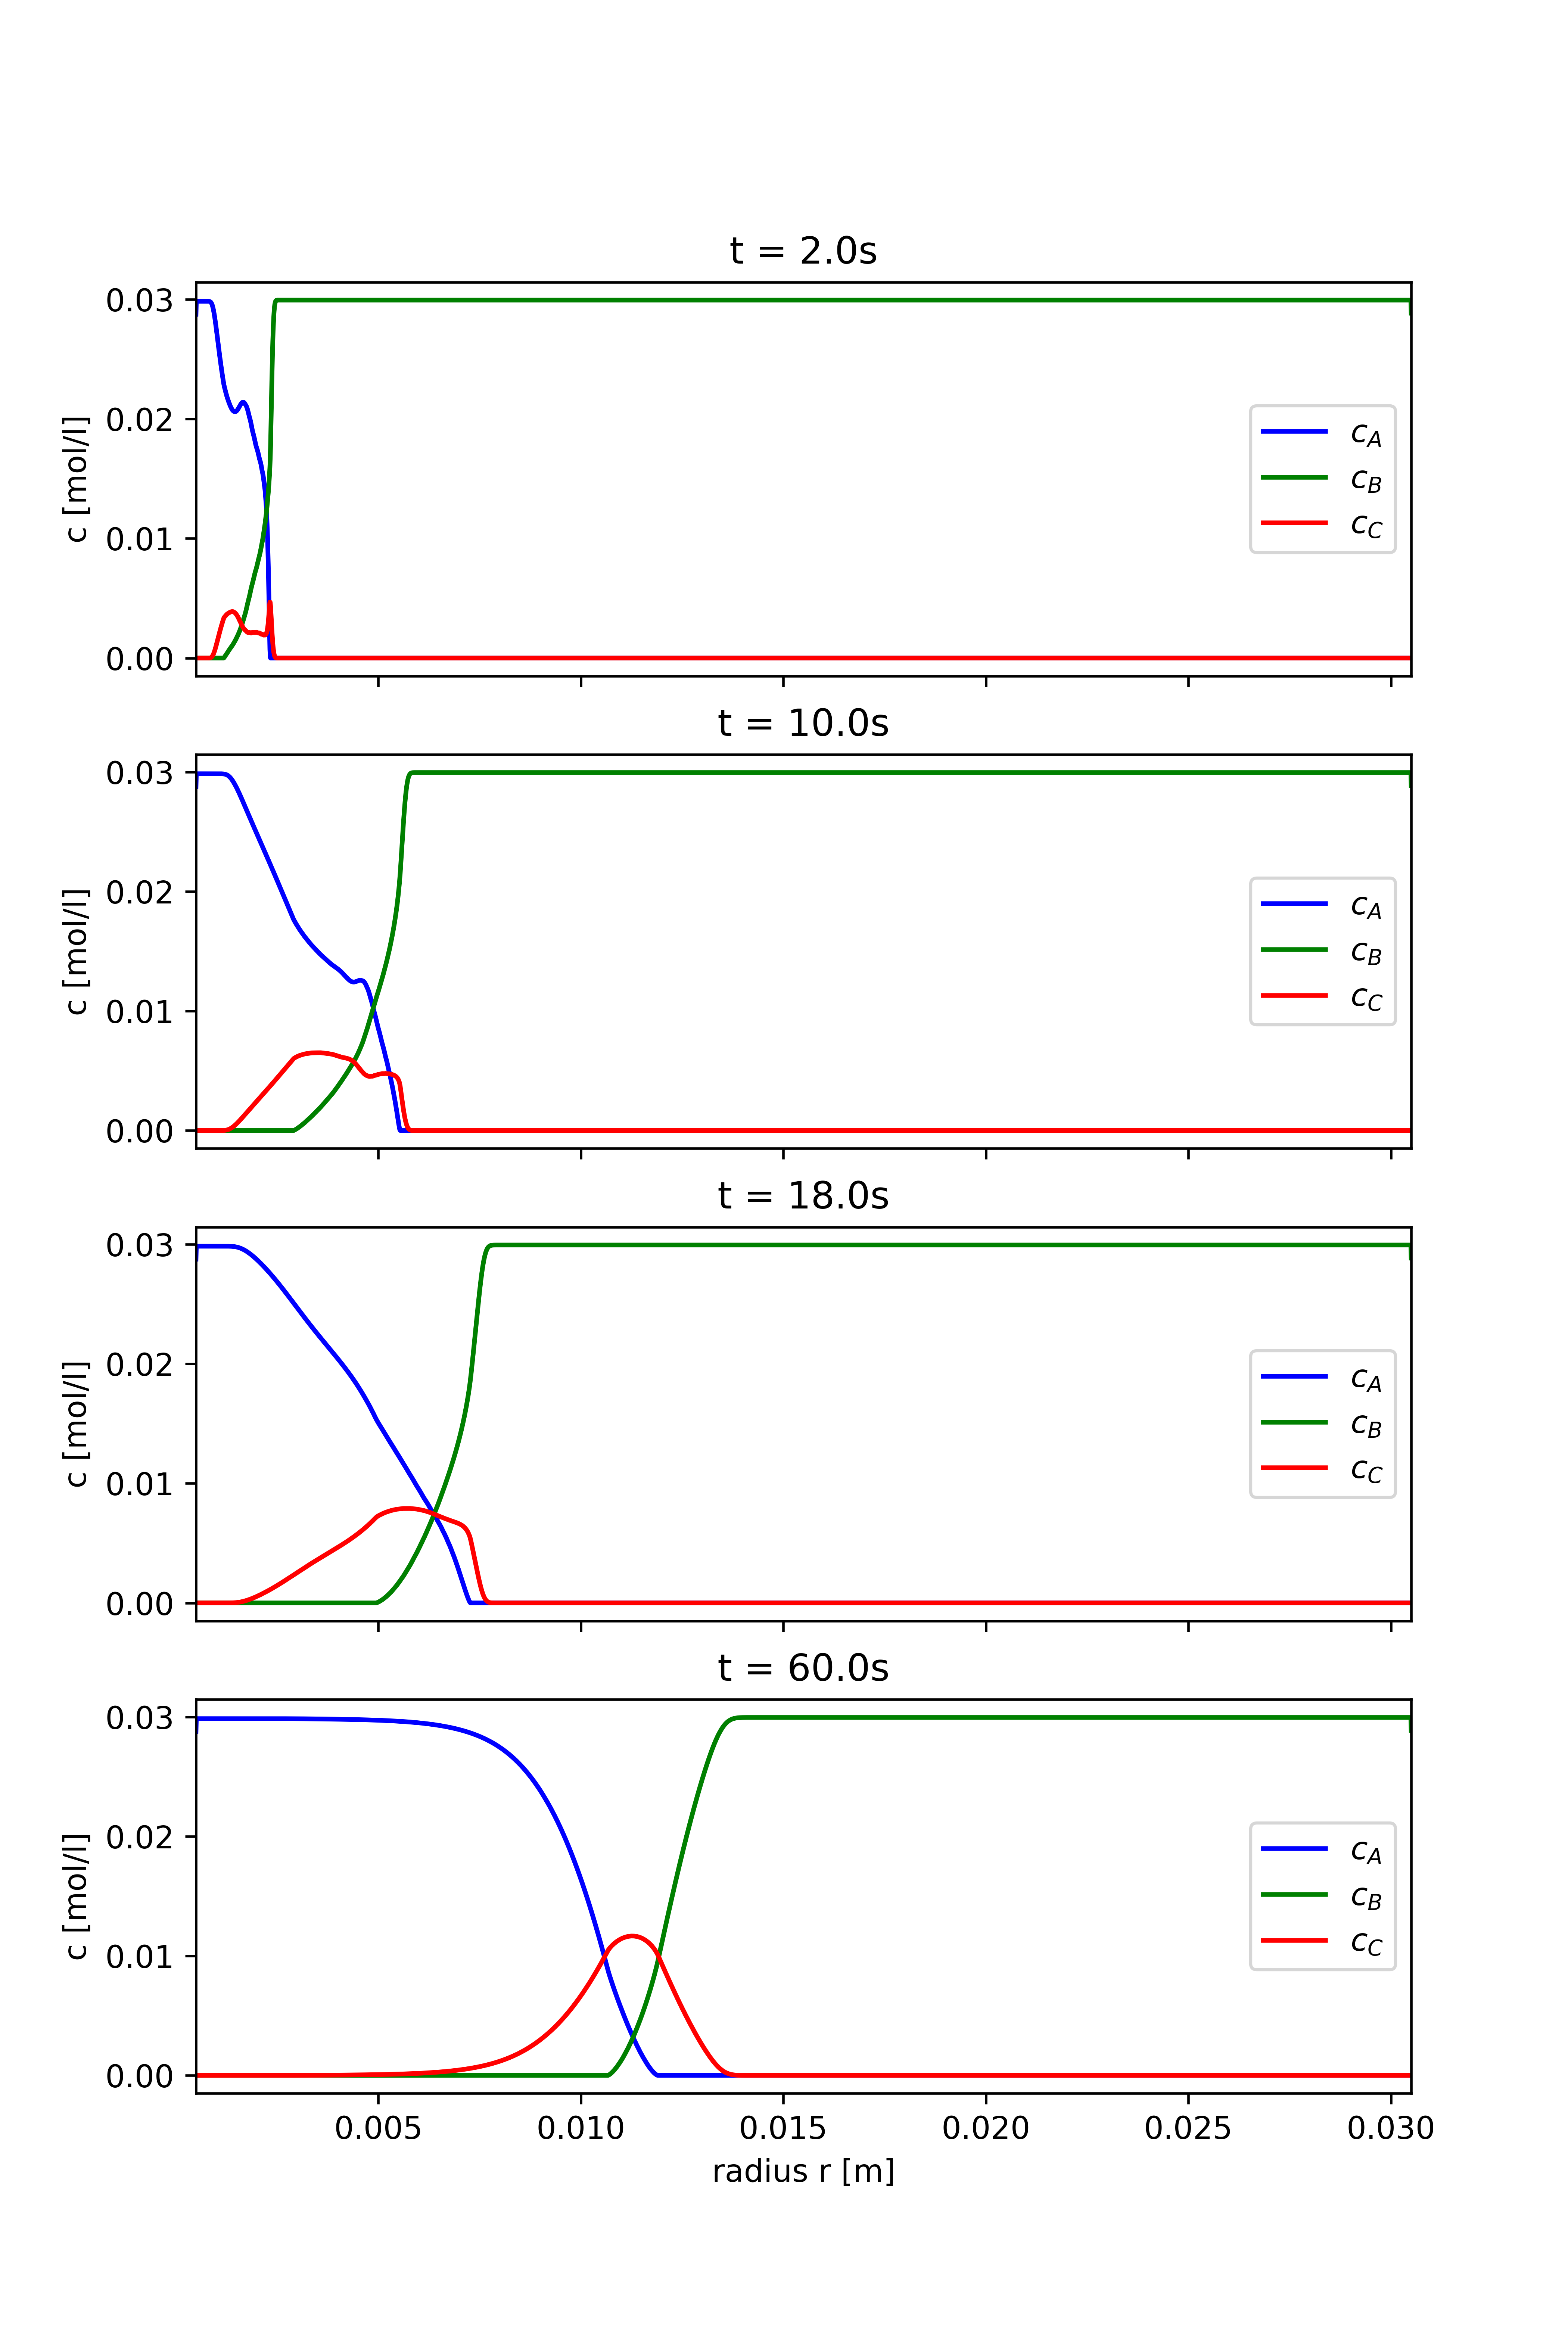
\includegraphics[width=.9\textwidth]{plot_h4r3_P205E3_S243E3_concentration-fluid_a_concentration-fluid_b_concentration-fluid_c}
	\caption{Plots for gap averaged concentrations for h = 0.4mm Pe = 2050 Sc = 2430}
	\label{fig: pos_h4_peak_plots}
\end{figure}
\begin{figure}[htbp]
	\centering
	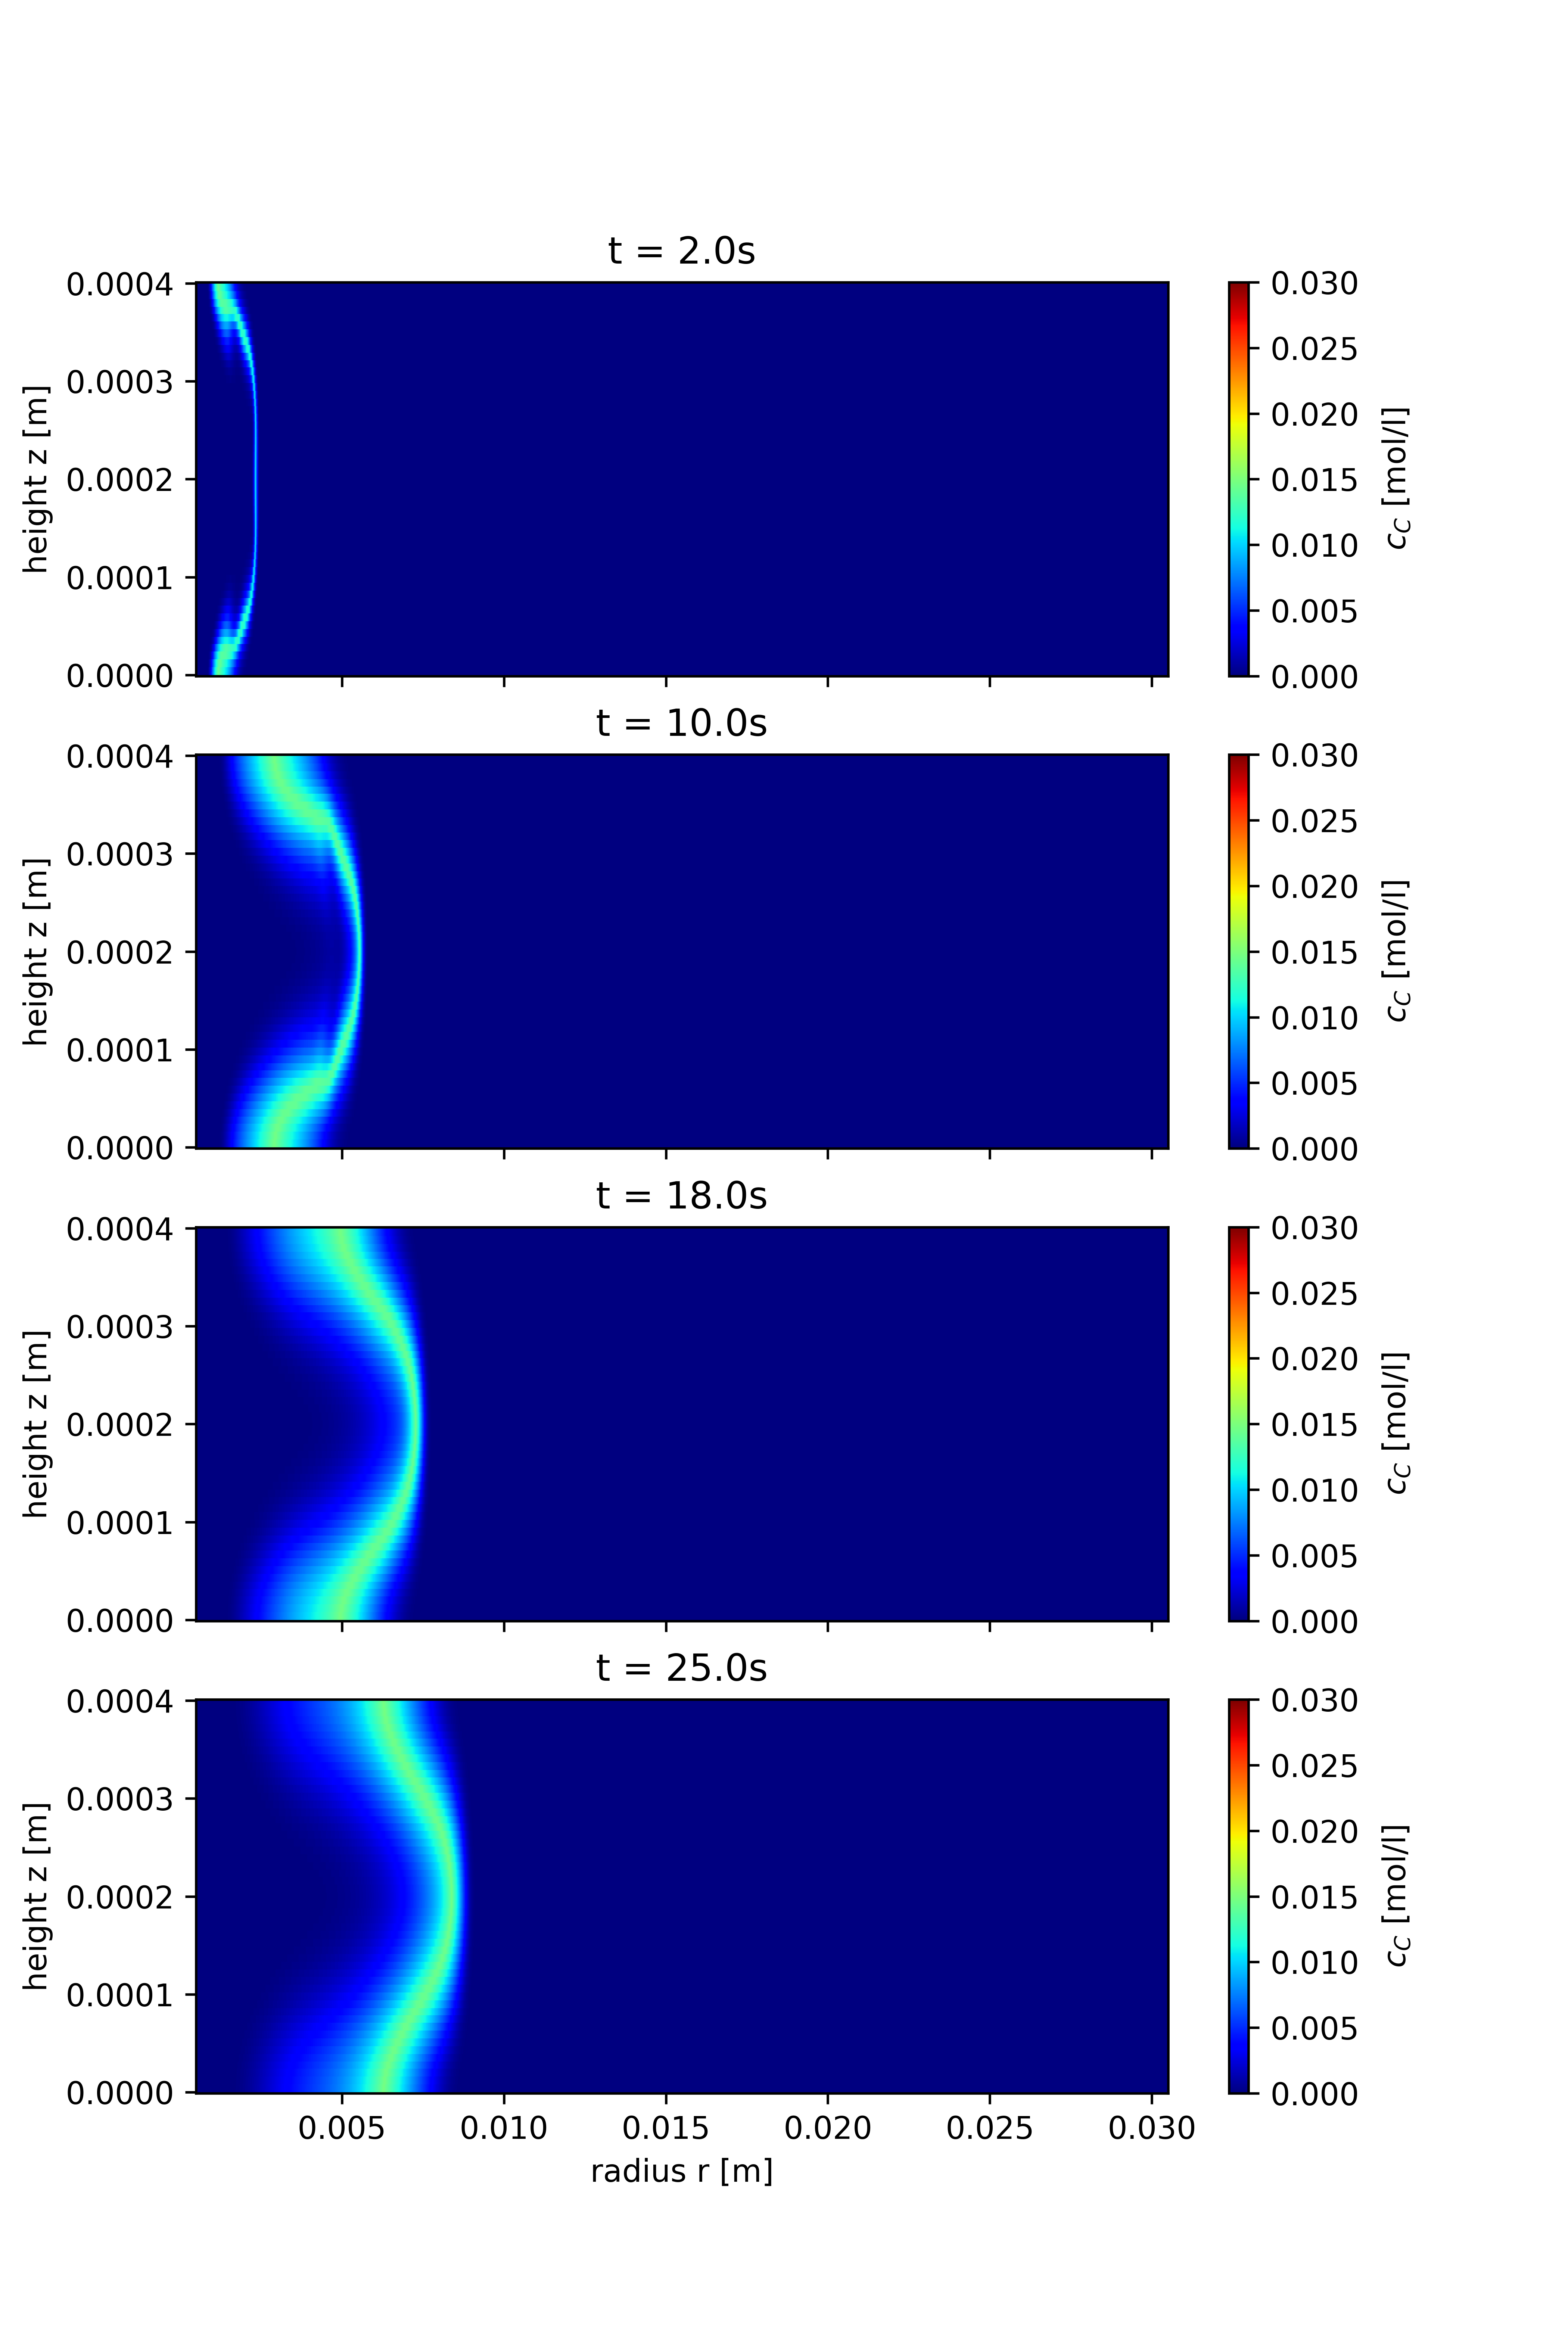
\includegraphics[width=.9\textwidth]{field_h4r3_P205E3_S243E3_concentration-fluid_c}
	\caption{Field for product concentration for h = 0.4mm Pe = 2050 Sc = 2430}
	\label{fig: pos_h4_peak_fields}
\end{figure}

At the time around 18 seconds the front shape has reached it's maximum distortion. Within the gap averaged plot it can be seen that there is a sharp increase at the fronts front and a slow decline at its back. This decline lowers when comparing the plots for a time of 18 seconds with the one at 60 seconds in \autoref{fig: pos_h4_peak_fields}.

The FWHMHGH behaviour can be explained using the local Peclet number. At early times the front is near the inlet, where the values are high so the influence of diffusion, which is the main mechanism driving the front's spreading is low. Diffusion along the radial direction is the main factor, because at half the gap height the flow does not experience any shear. Advection is mainly moving the front through the reactor. While leaving the advection influence zone the FWHMHGH starts growing more rapidly, since diffusion start more and more dominating the width's growth process. The width's growths then slows down and reaches a constant value due the fact, that an equilibrium between diffusion and the reaction is reached. The differences in the FWHMHGH curves, when comparing different Schmidt numbers, can be explained by different diffusion coefficients. The higher the diffusion coefficient the sooner the growth starts and the final constant value is reached sooner as well.
\newpage

For the case with a gap height of 0.6mm the width's behaviour seems to change quite significantly compared to the 0.4mm case. 
\begin{figure}[htb]
	\centering
	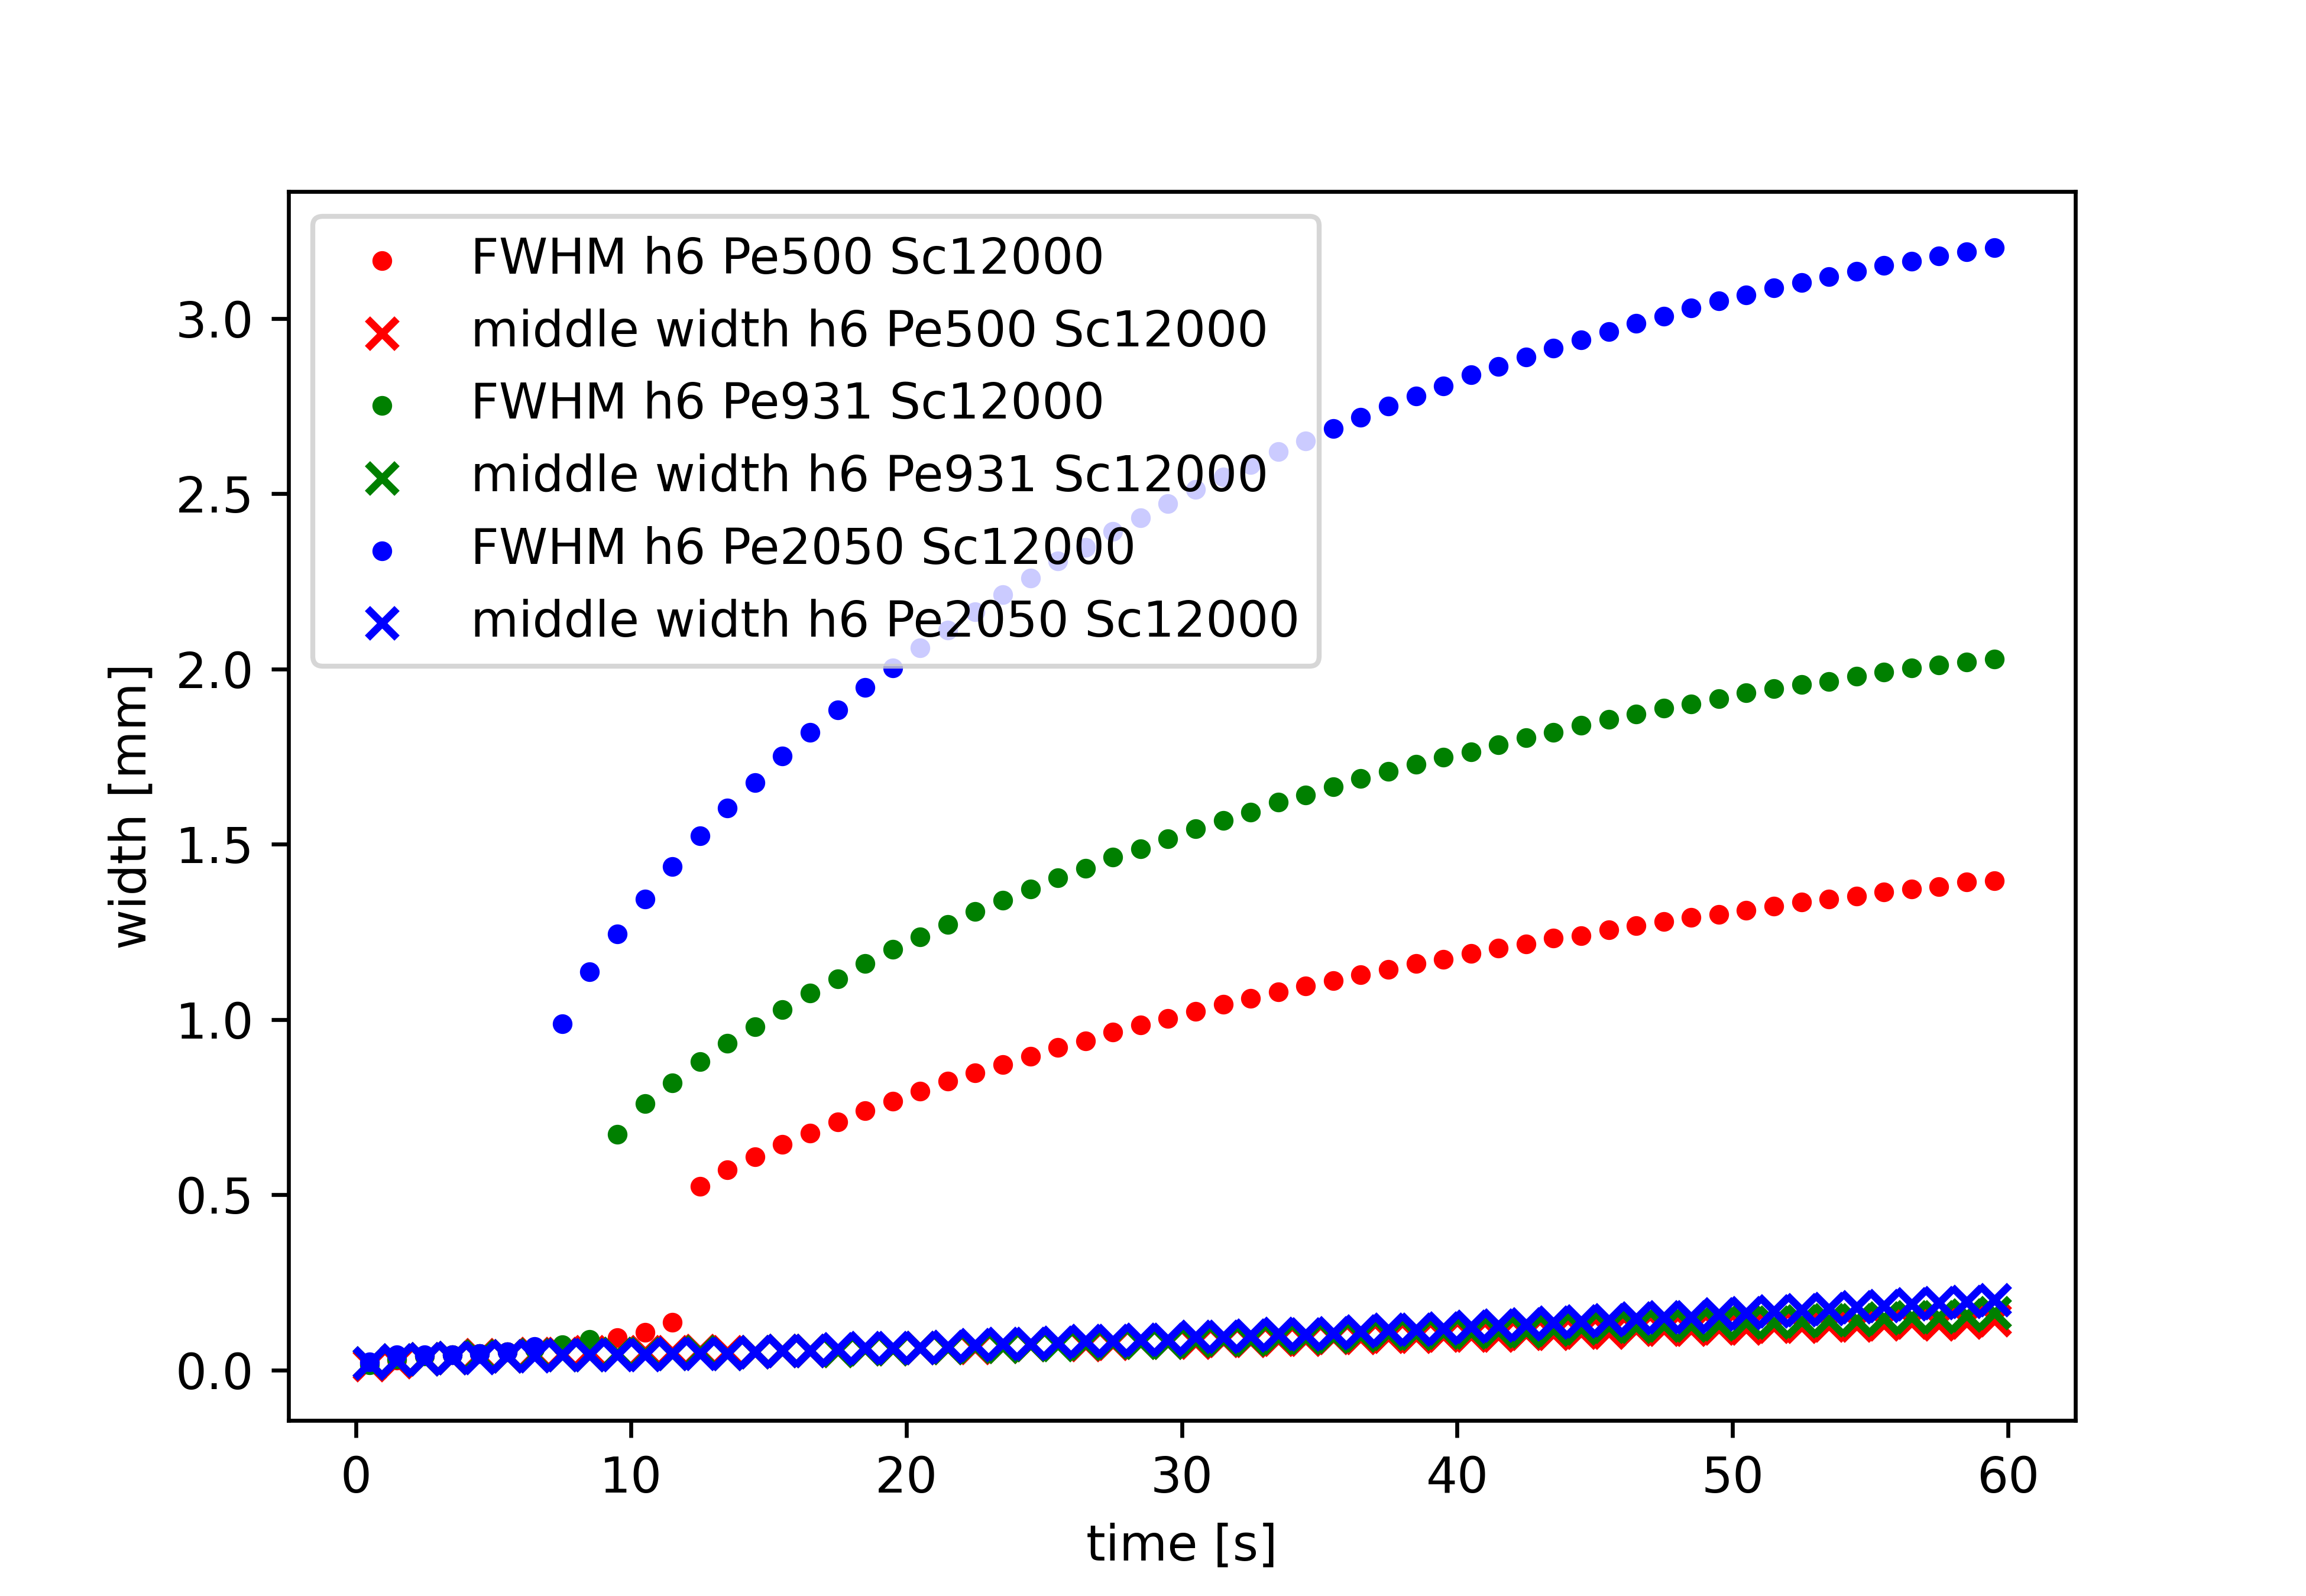
\includegraphics[width=.9\linewidth]{front_width_h6_Sc12000}
	\caption{Front widths for  h = 0.6mm Sc = 12000}
	\label{fig: front_width_h6_Sc12000}
\end{figure}
For the Schmidt number of 12000 the width's results are shown in \autoref{fig: front_width_h6_Sc12000}. The general form of the FWHM curves seems to match the ones from the previous discussed cases. A difference, compared to the 0.4mm cases, is that the width's growth seems to start delayed even more at around 8 to 12 seconds. The FWHMHGH does not grow at all for this Schmidt number.
\begin{figure}[htb]
	\centering
	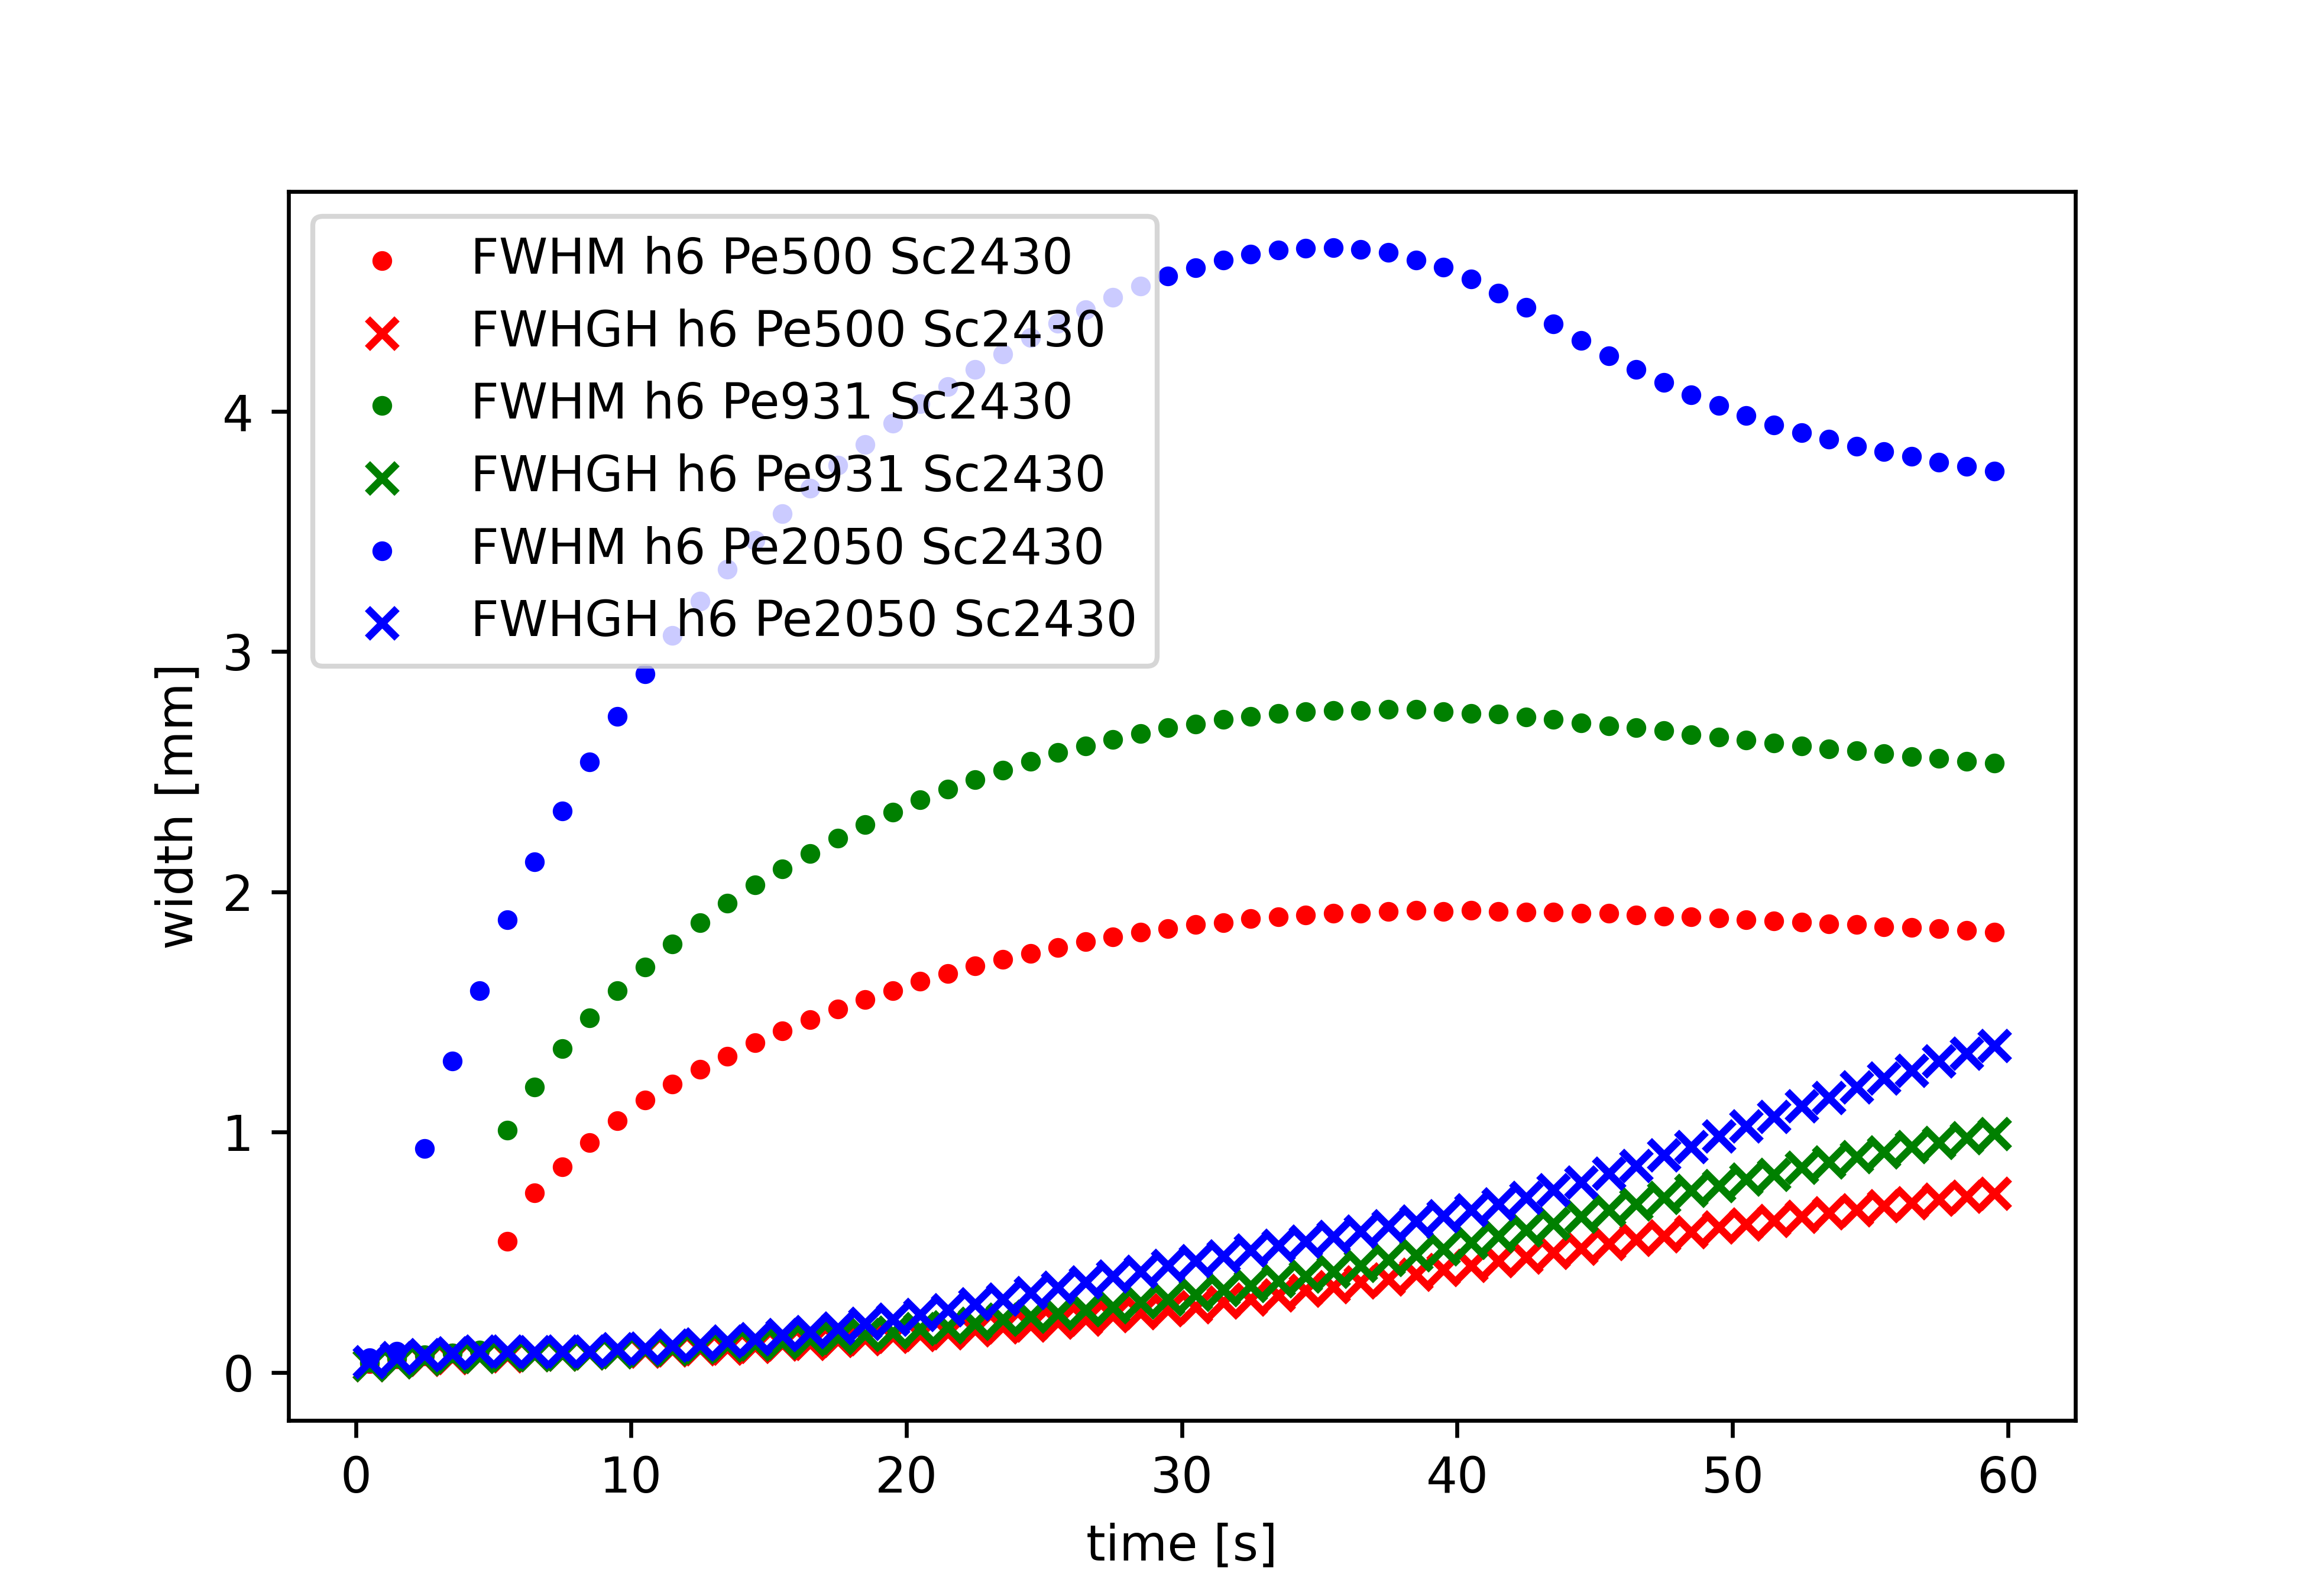
\includegraphics[width=.9\linewidth]{front_width_h6_Sc2430}
	\caption{Front widths for  h = 0.6mm Sc = 2430}
	\label{fig: front_width_pos_h6_Sc2430}
\end{figure}
For the lower Schmidt number, shown in \autoref{fig: front_width_pos_h6_Sc2430}, the peak within the FWHM plot widens even more compared to the previous cases and the maximum value is reached at later times. The FWHMHGH does not grow a lot for the first 20 seconds, but after that the widths growth rate starts increasing.

The growth delay, that can be seen for the Schmidt number of 12000 for the gap height of 0.4mm in \autoref{fig: front_width_h4_Sc12000} and for the same Schmidt number for a gap height of 0.6mm in \autoref{fig: front_width_h6_Sc12000}, can be explained using the concentration plots. Within \autoref{fig: plots_early} the concentration plots are shown for the gap height of 0.4mm and 0.6mm for a Peclet number of 931 and a Schmidt number of 12000 close to the inlet. Within these two plots it can seen that the initial spike in the front start decaying over time. The moment the value of $0\text{.}5 \cdot c_{c,max}$ falls into the region above 0 and below the value at the back of the front, the front's width suddenly increases to a higher value.
\begin{figure}[htb]
	\centering
	\subfloat[\centering  h = 0.6mm case]{{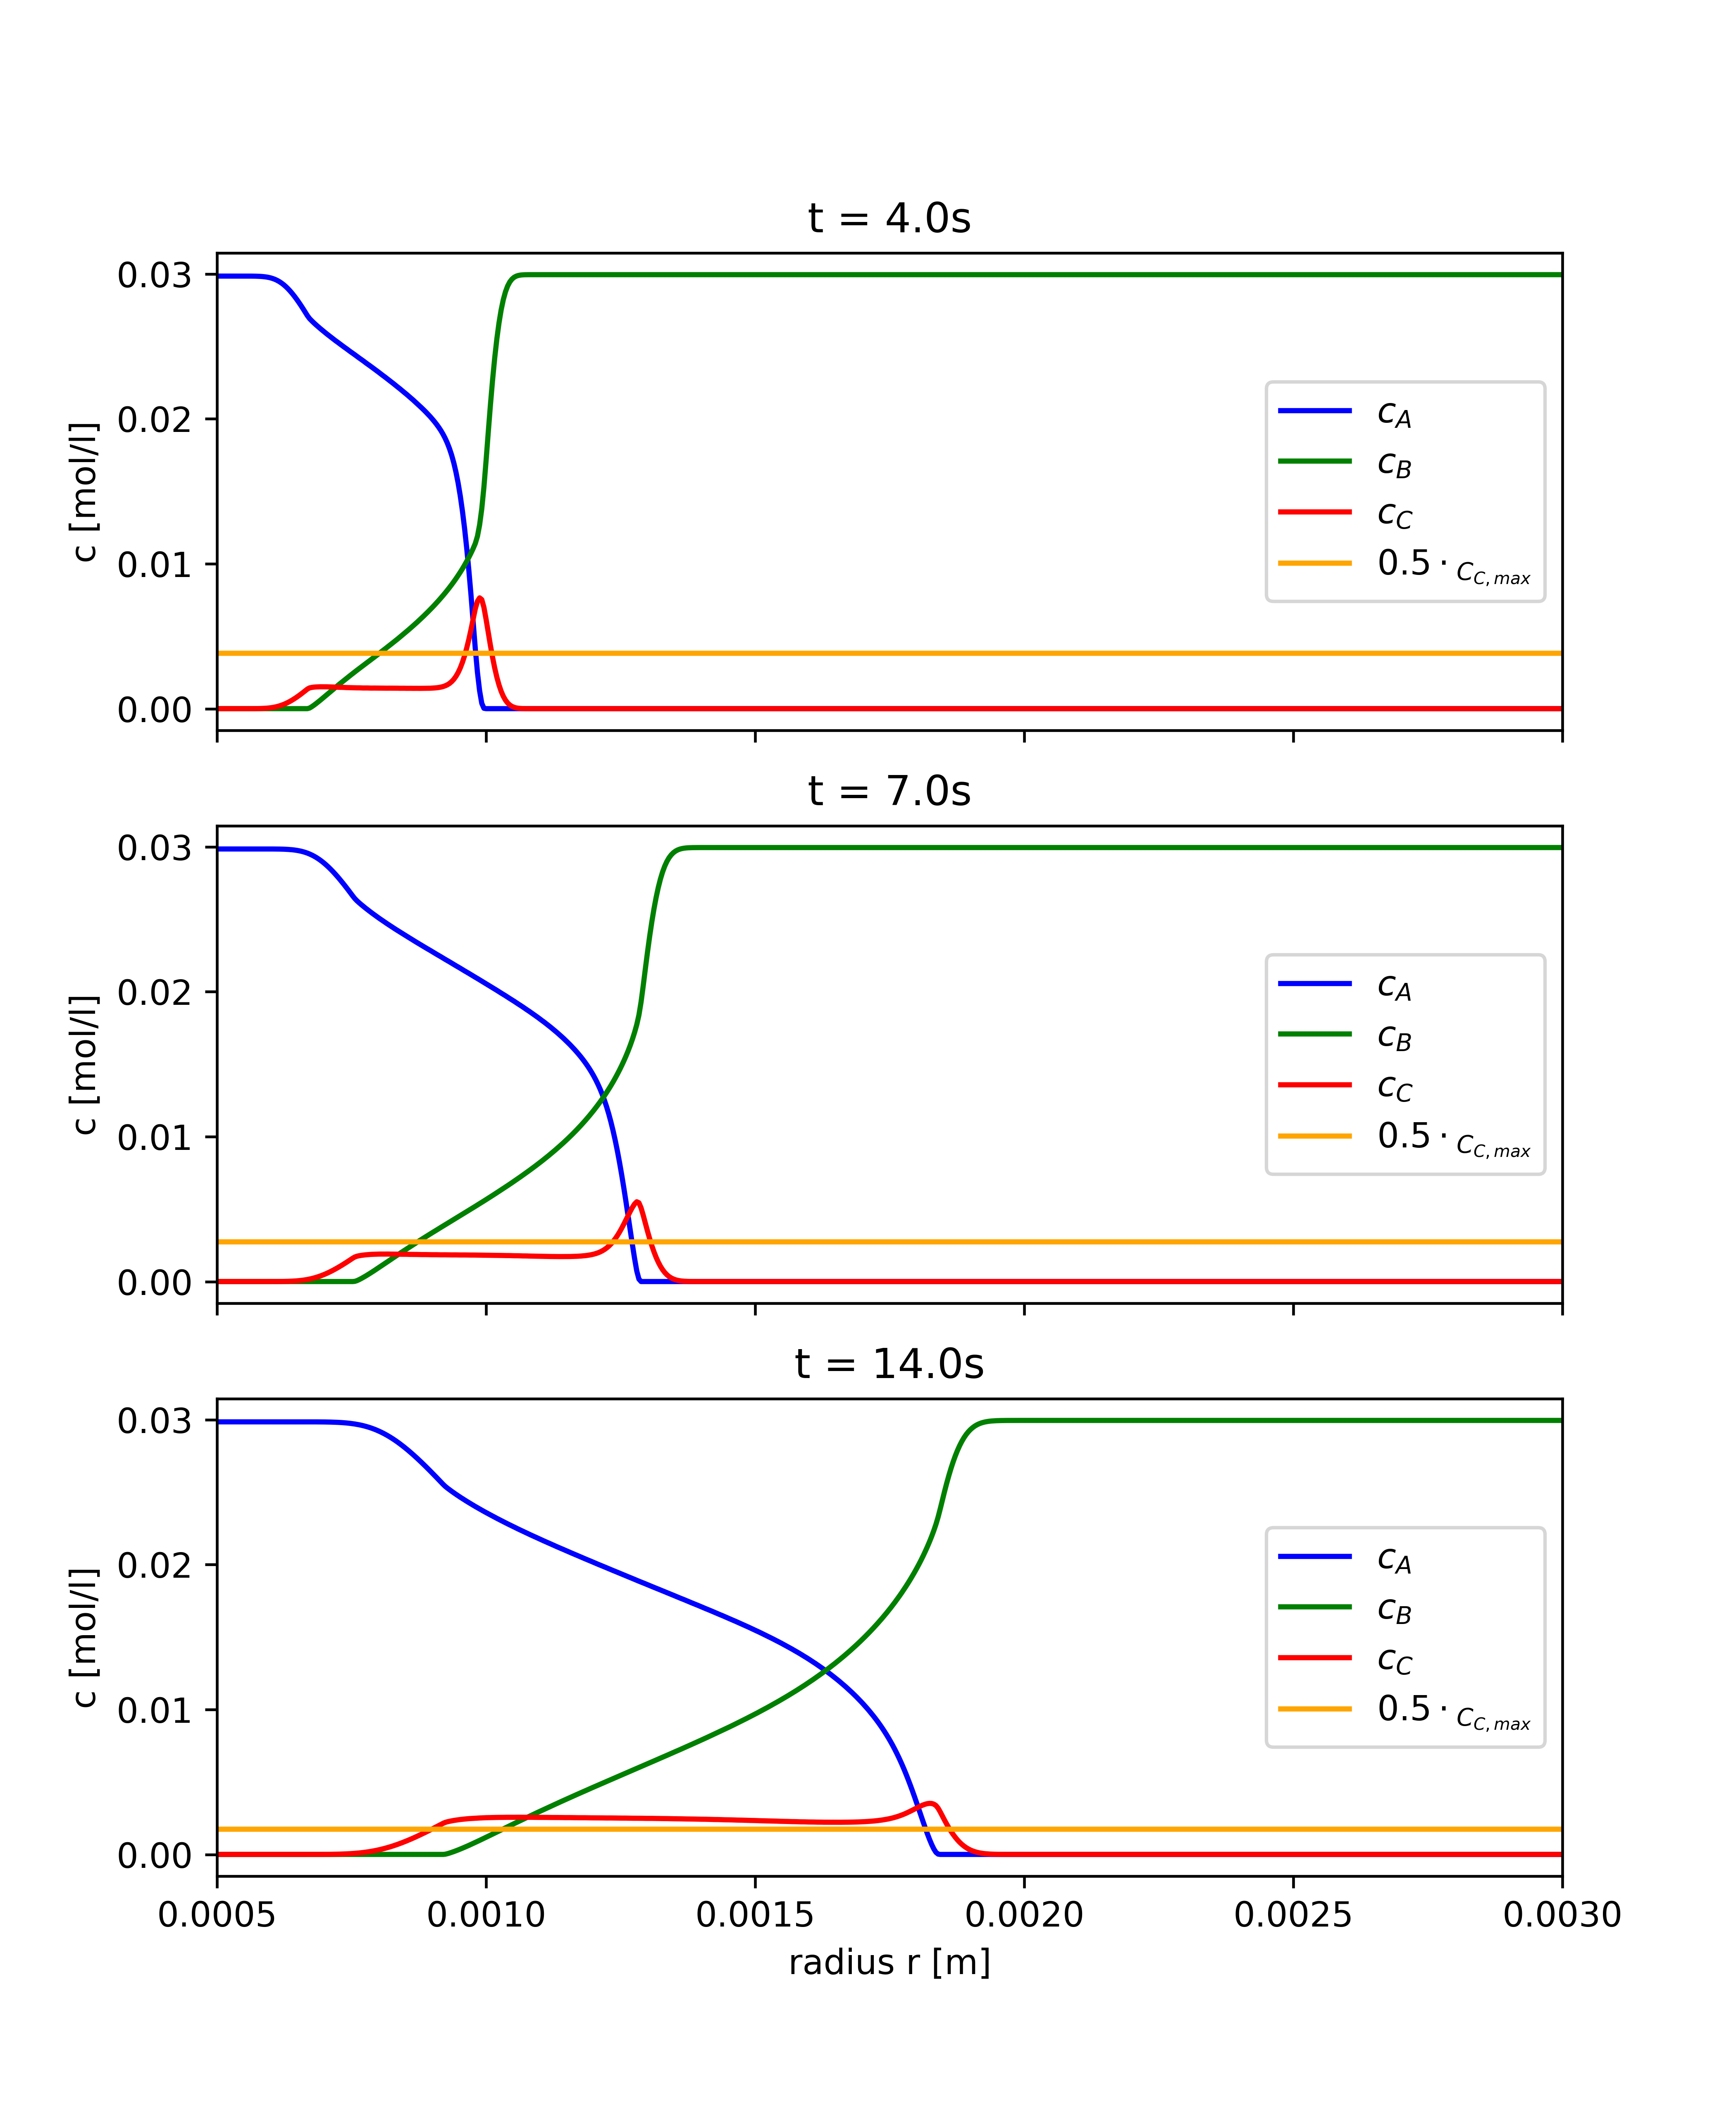
\includegraphics[angle=0, scale=0.41]{plot_h6r3_P931E2_S120E4_concentration-fluid_a_concentration-fluid_b_concentration-fluid_c} }}%
	\qquad
	\subfloat[\centering  h = 0.4mm case]{{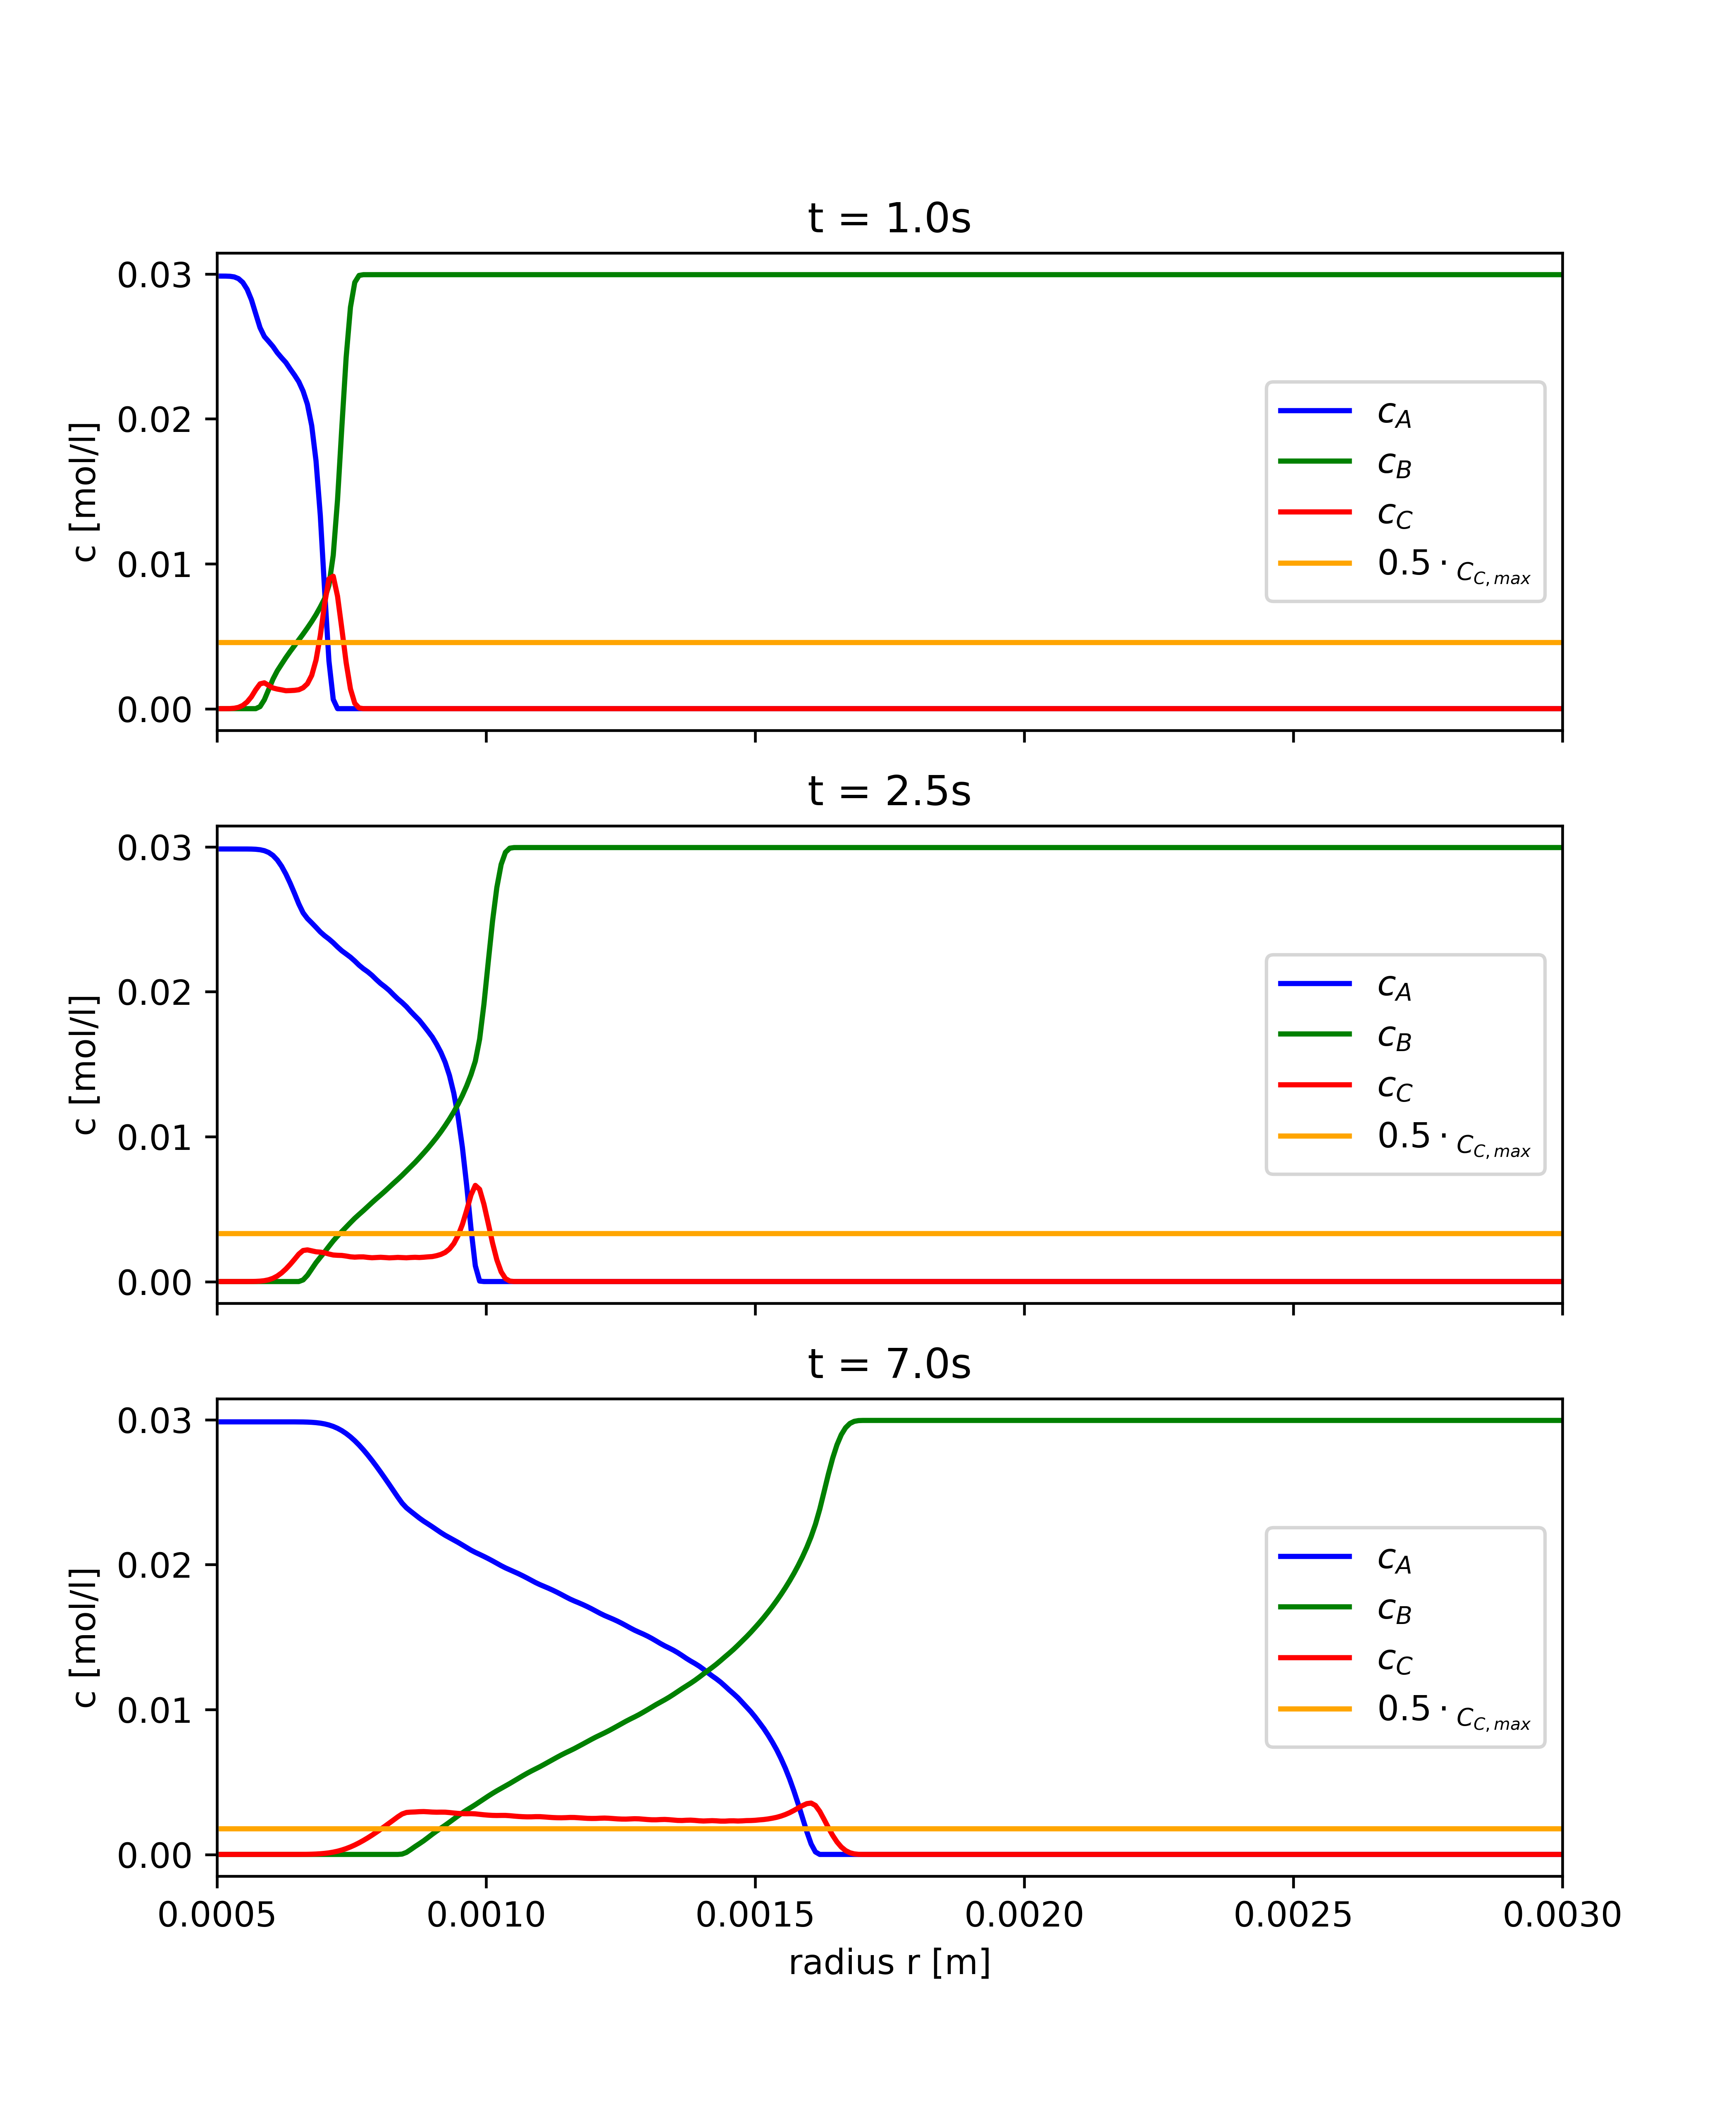
\includegraphics[angle=0, scale=0.41]{plot_h4r3_P931E2_S120E4_concentration-fluid_a_concentration-fluid_b_concentration-fluid_c copy} }}%
	\caption{Concentration plots for  Pe = 931 Sc = 12000}%
	\label{fig: plots_early}%
\end{figure}
The FWHMHGH only reaches very low values and doesn't grow much within the 60 seconds runtime of the simulation. The reason for that behaviour is the same as discussed for the 0.4mm case. The influence of diffusion starts dominating the front's spreading at later radial values, due to a higher local Peclet number near the inlet. In the case of the higher Schmidt number the diffusion process does not seem get starting within the 60 second timespan of the simulation, because the coefficient has a low value.
\newline 

All in all the front widths show different behaviour dependent on the conditions set for the cases. Changing the Schmidt number poses a significant change within the results as showed and discussed. The main influence is the diffusion coefficient that has an effect on where and when the front's width growth starts to happen. The Peclet number seems to mostly influence the width's maximum peak value but doesn't change the general behaviour of the front. That is the case, because the Peclet number mostly influences the input velocity, which influences the distortion of the front.

\section{Formed Product}

Within this section the total product formed is investigated. 

\begin{figure}[htb]
	\centering
	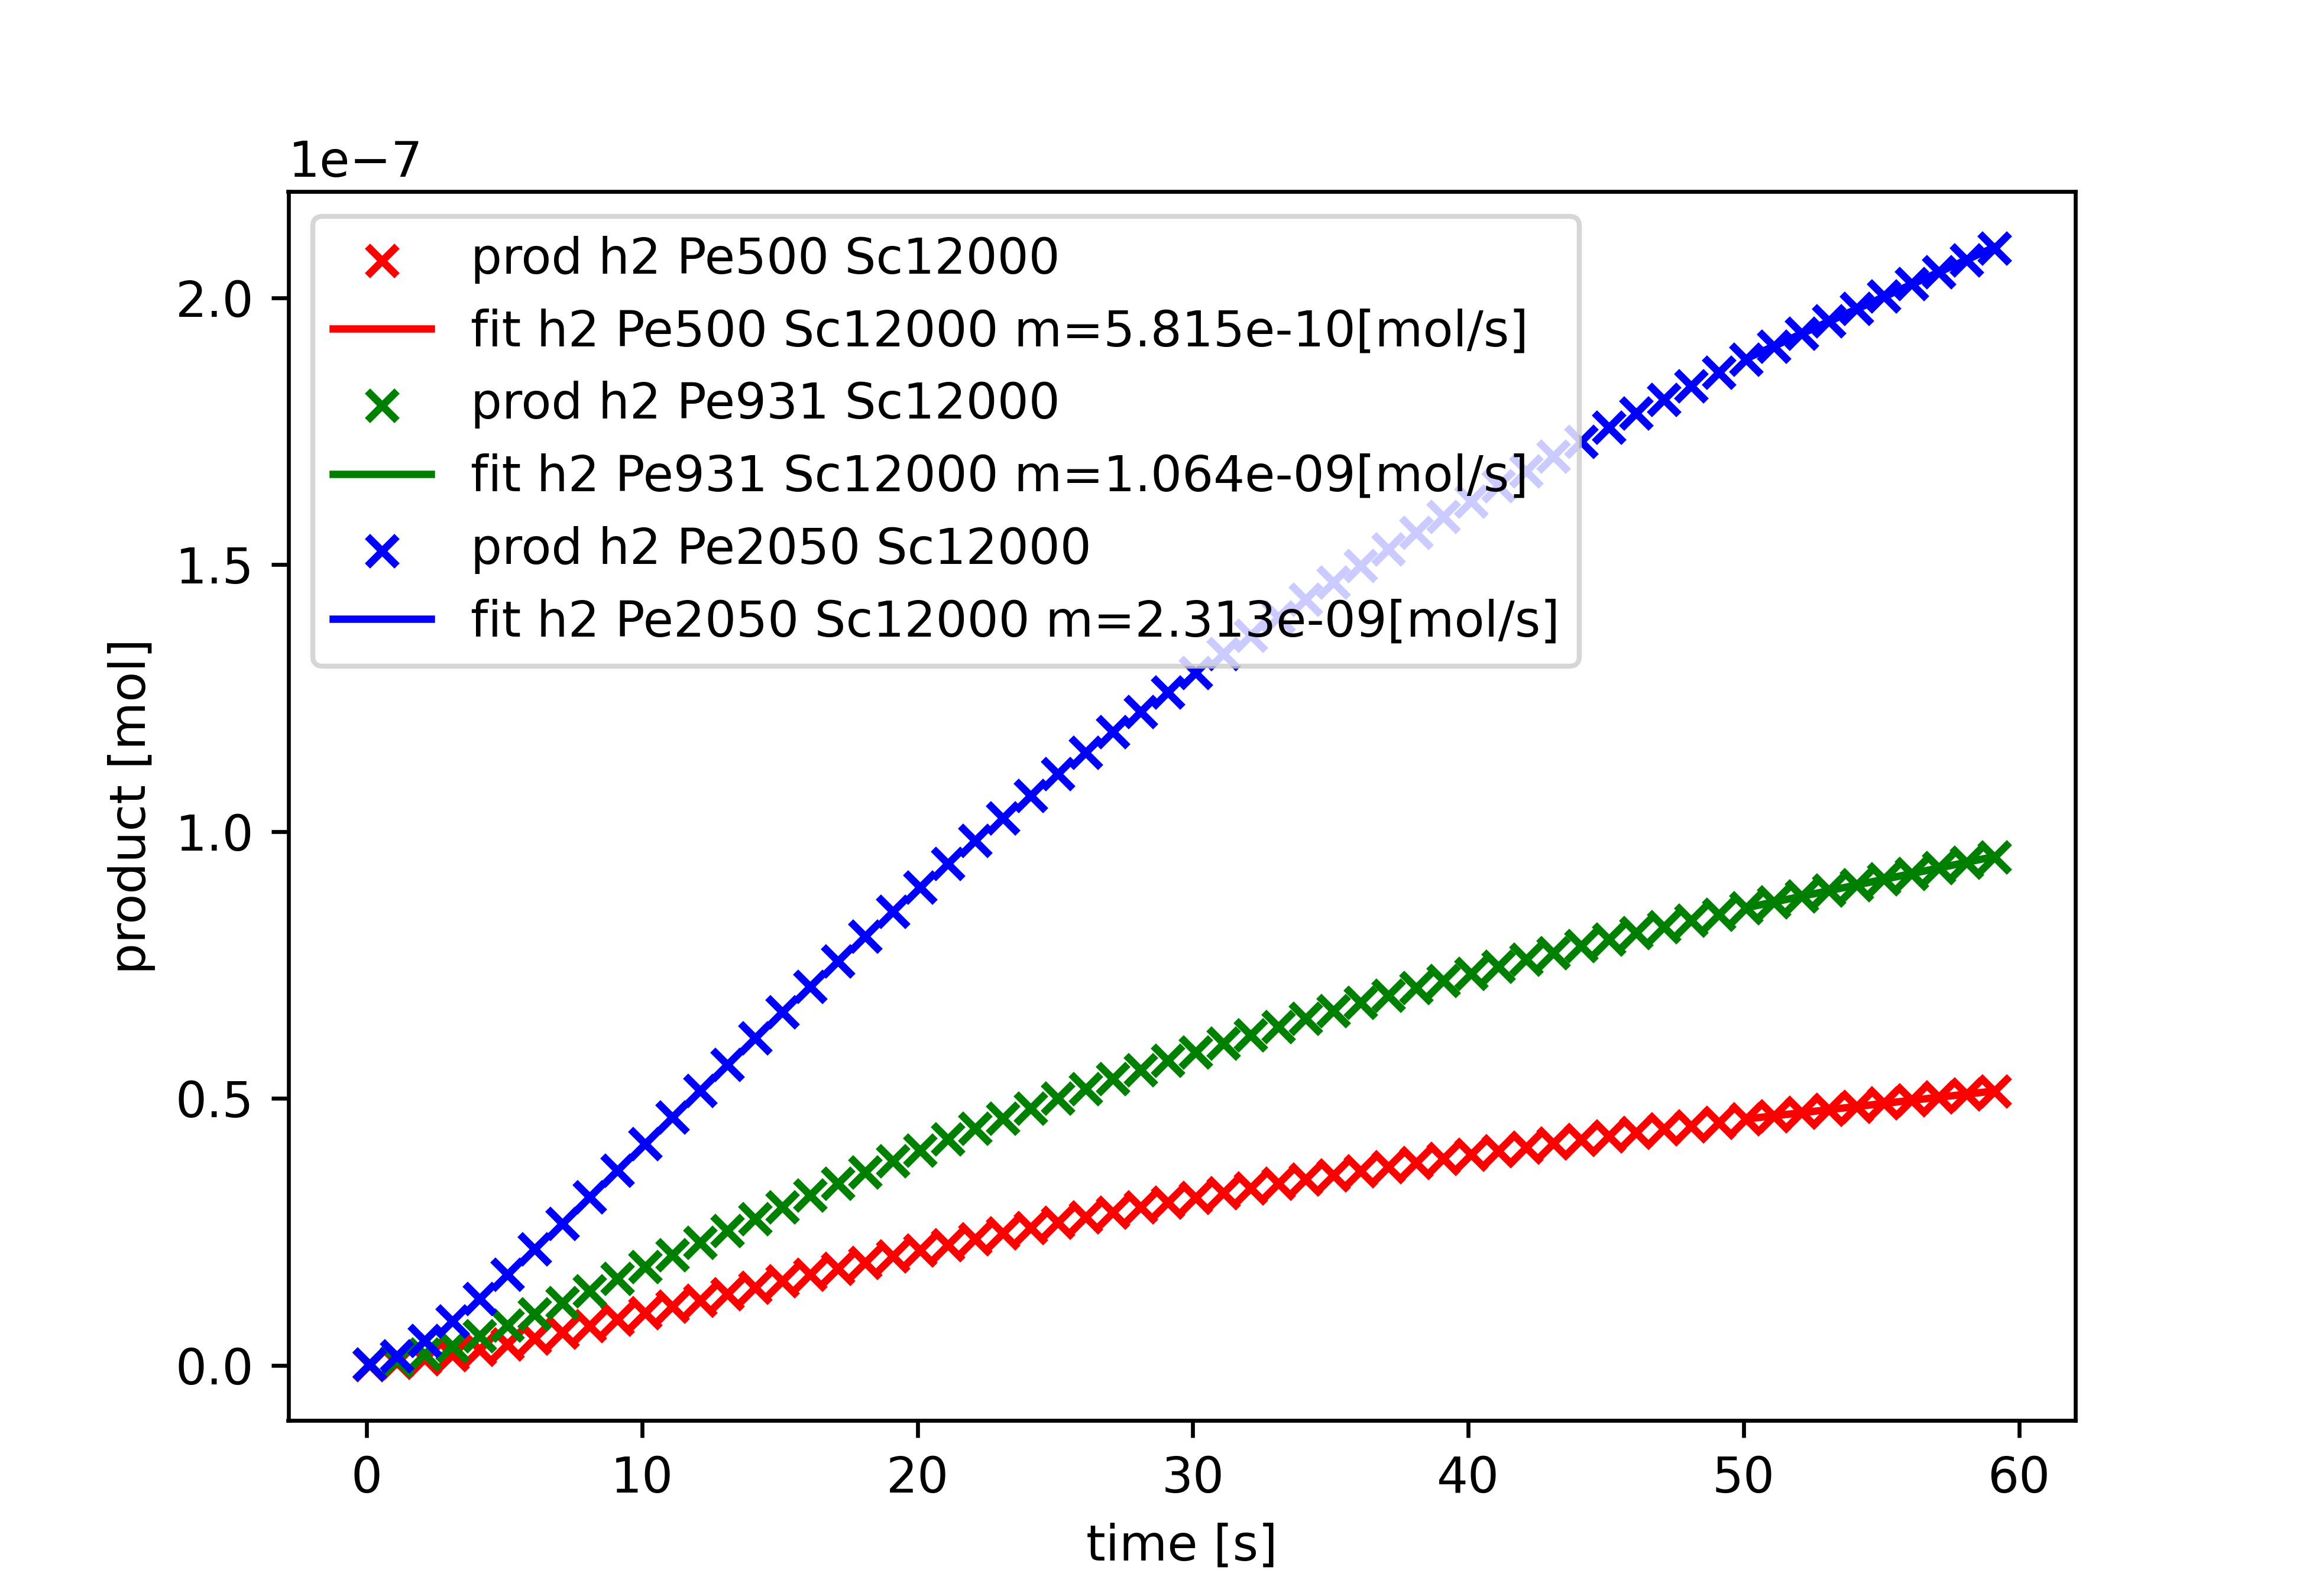
\includegraphics[width=.9\linewidth]{total_product_h2_Sc12000}
	\caption{Total amount of product for h = 0.2mm Sc = 12000}
	\label{fig: total_prod_h2_Sc12000}
\end{figure}
For the case with a gap height of 0.2mm the total product formed starts with a linear growth which then slowly decays for all cases with a Schmidt number of 12000.
\begin{figure}[htb]
	\centering
	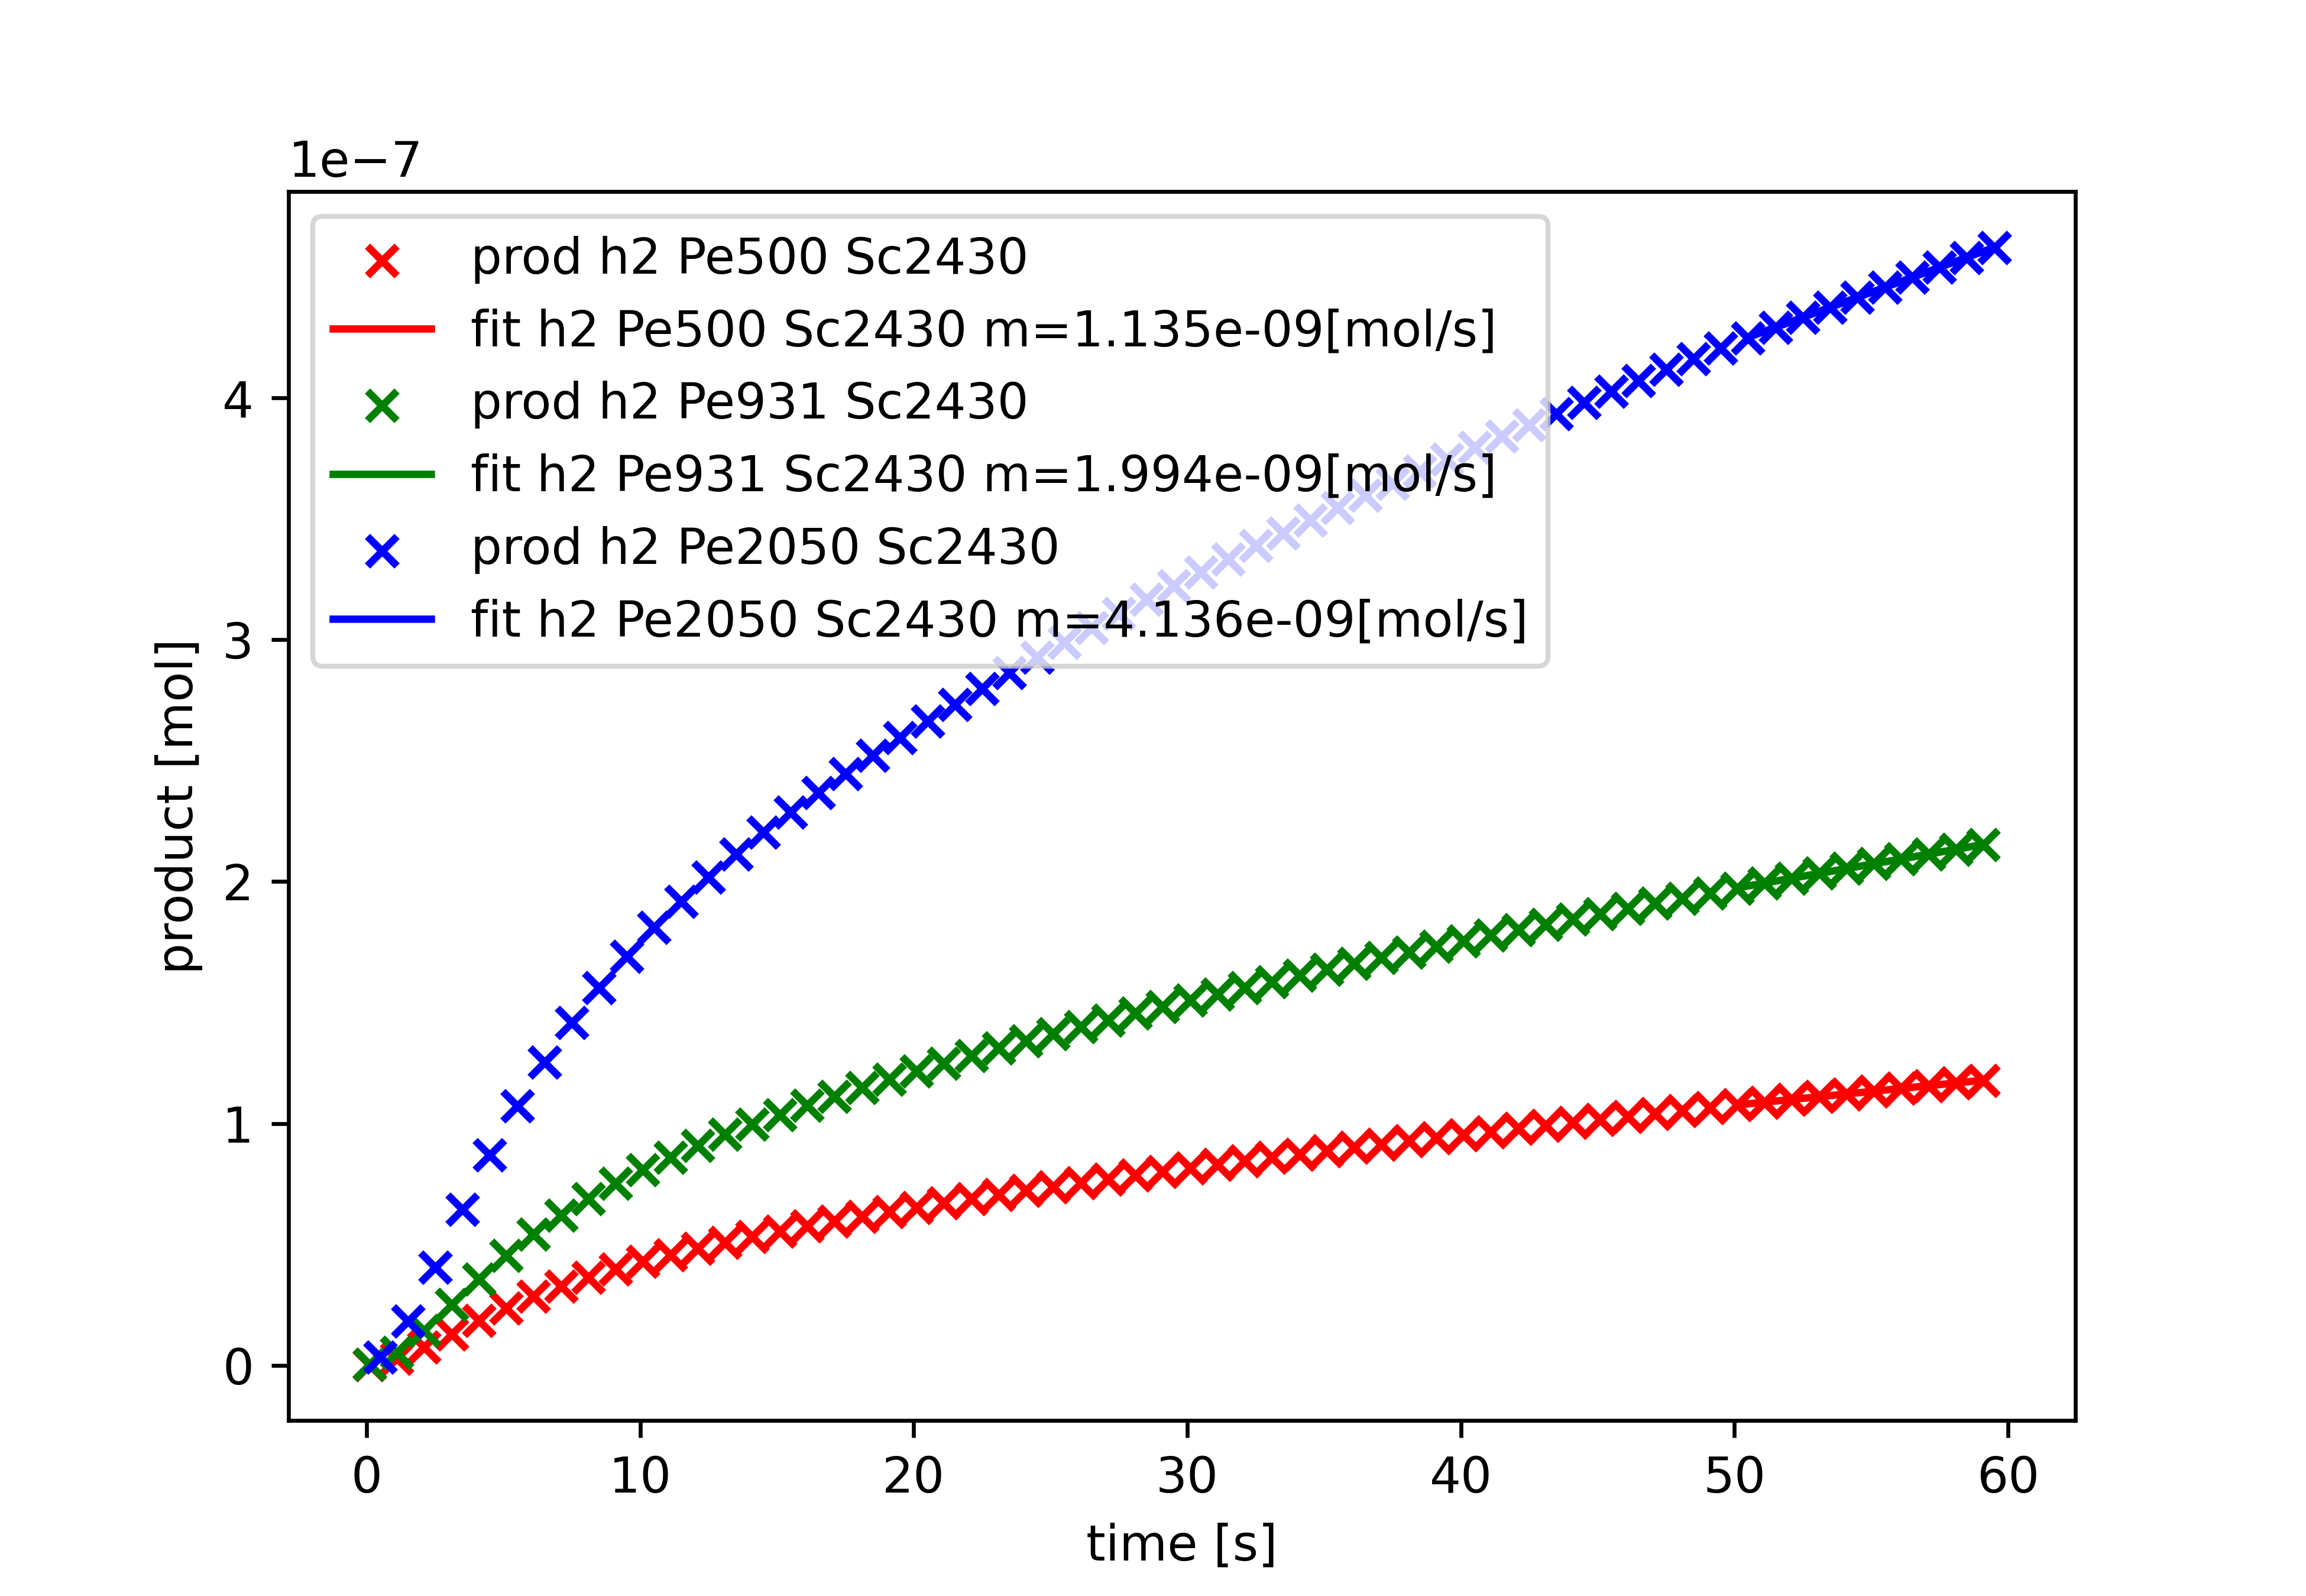
\includegraphics[width=.9\linewidth]{total_product_h2_Sc2430}
	\caption{Total product for  h = 0.2mm Sc = 2430}
	\label{fig: total_prod_h2_Sc2430}
\end{figure}
The difference when lowering the Schmidt number, is that the initial production rate is higher and the decay starts earlier. In addition to the plot of the product $C$ in mol against time in seconds, a linear fit is done with the data of the last 10 seconds. The fit approach is shown in \autoref{eqn: prod_fit}.
\begin{equation}
	\label{eqn: prod_fit}
	n_C \left[ \text{mol} \right] = m \left[\frac{\text{mol}}{\text{s}}\right] \cdot t \left[s\right] + b \left[mol\right]
\end{equation}
Since only the production rate $m$ is of interest, only it's values are included in the diagrams.

The curve's shapes can be explained by looking at the influence of advection and diffusion. For the higher Schmidt number of 12000 the production rate only slightly lowers over the 60 seconds of simulation time. At the start of the simulation the front's shape is very narrow. The reactants $A$ and $B$ need to travel via diffusion through the front to form the product $C$. Since the diffusion coefficient is low the reaction rate in the beginning is also quite low. With time passing the fronts width gets wider and the distance the reactants have to travel grows. That is why the production rate decreases. The final value it reaches is dependant on the equilibrium that is build between the diffusion and the reaction process. With higher Peclet numbers the fronts distortion gets higher so new surface area is generated for the reaction to take place. That is a reason why the reaction rate is higher for higher Peclet numbers.
The same arguments can be used to explain, why the initial production rate is high and then decreases for the cases with a Schmidt number of 2340. The higher diffusion coefficient in combination with the narrow front lead to this high production rate. The production rate at the end of the simulation is also affected by this showing nearly twice as high values for the lower Schmidt number cases of \autoref{fig: total_prod_h2_Sc12000} compared against the higher Schmidt number ones of \autoref{fig: total_prod_h2_Sc2430}.
\newline

The total amount of product behaves very similar for the gap height of 0.4mm and 0.6mm. For that reason only the 0.4mm cases are analysed here. The results for the 0.6mm cases can be found in Section \ref{sec: app_prodrate}.
\begin{figure}[htb]
	\centering
	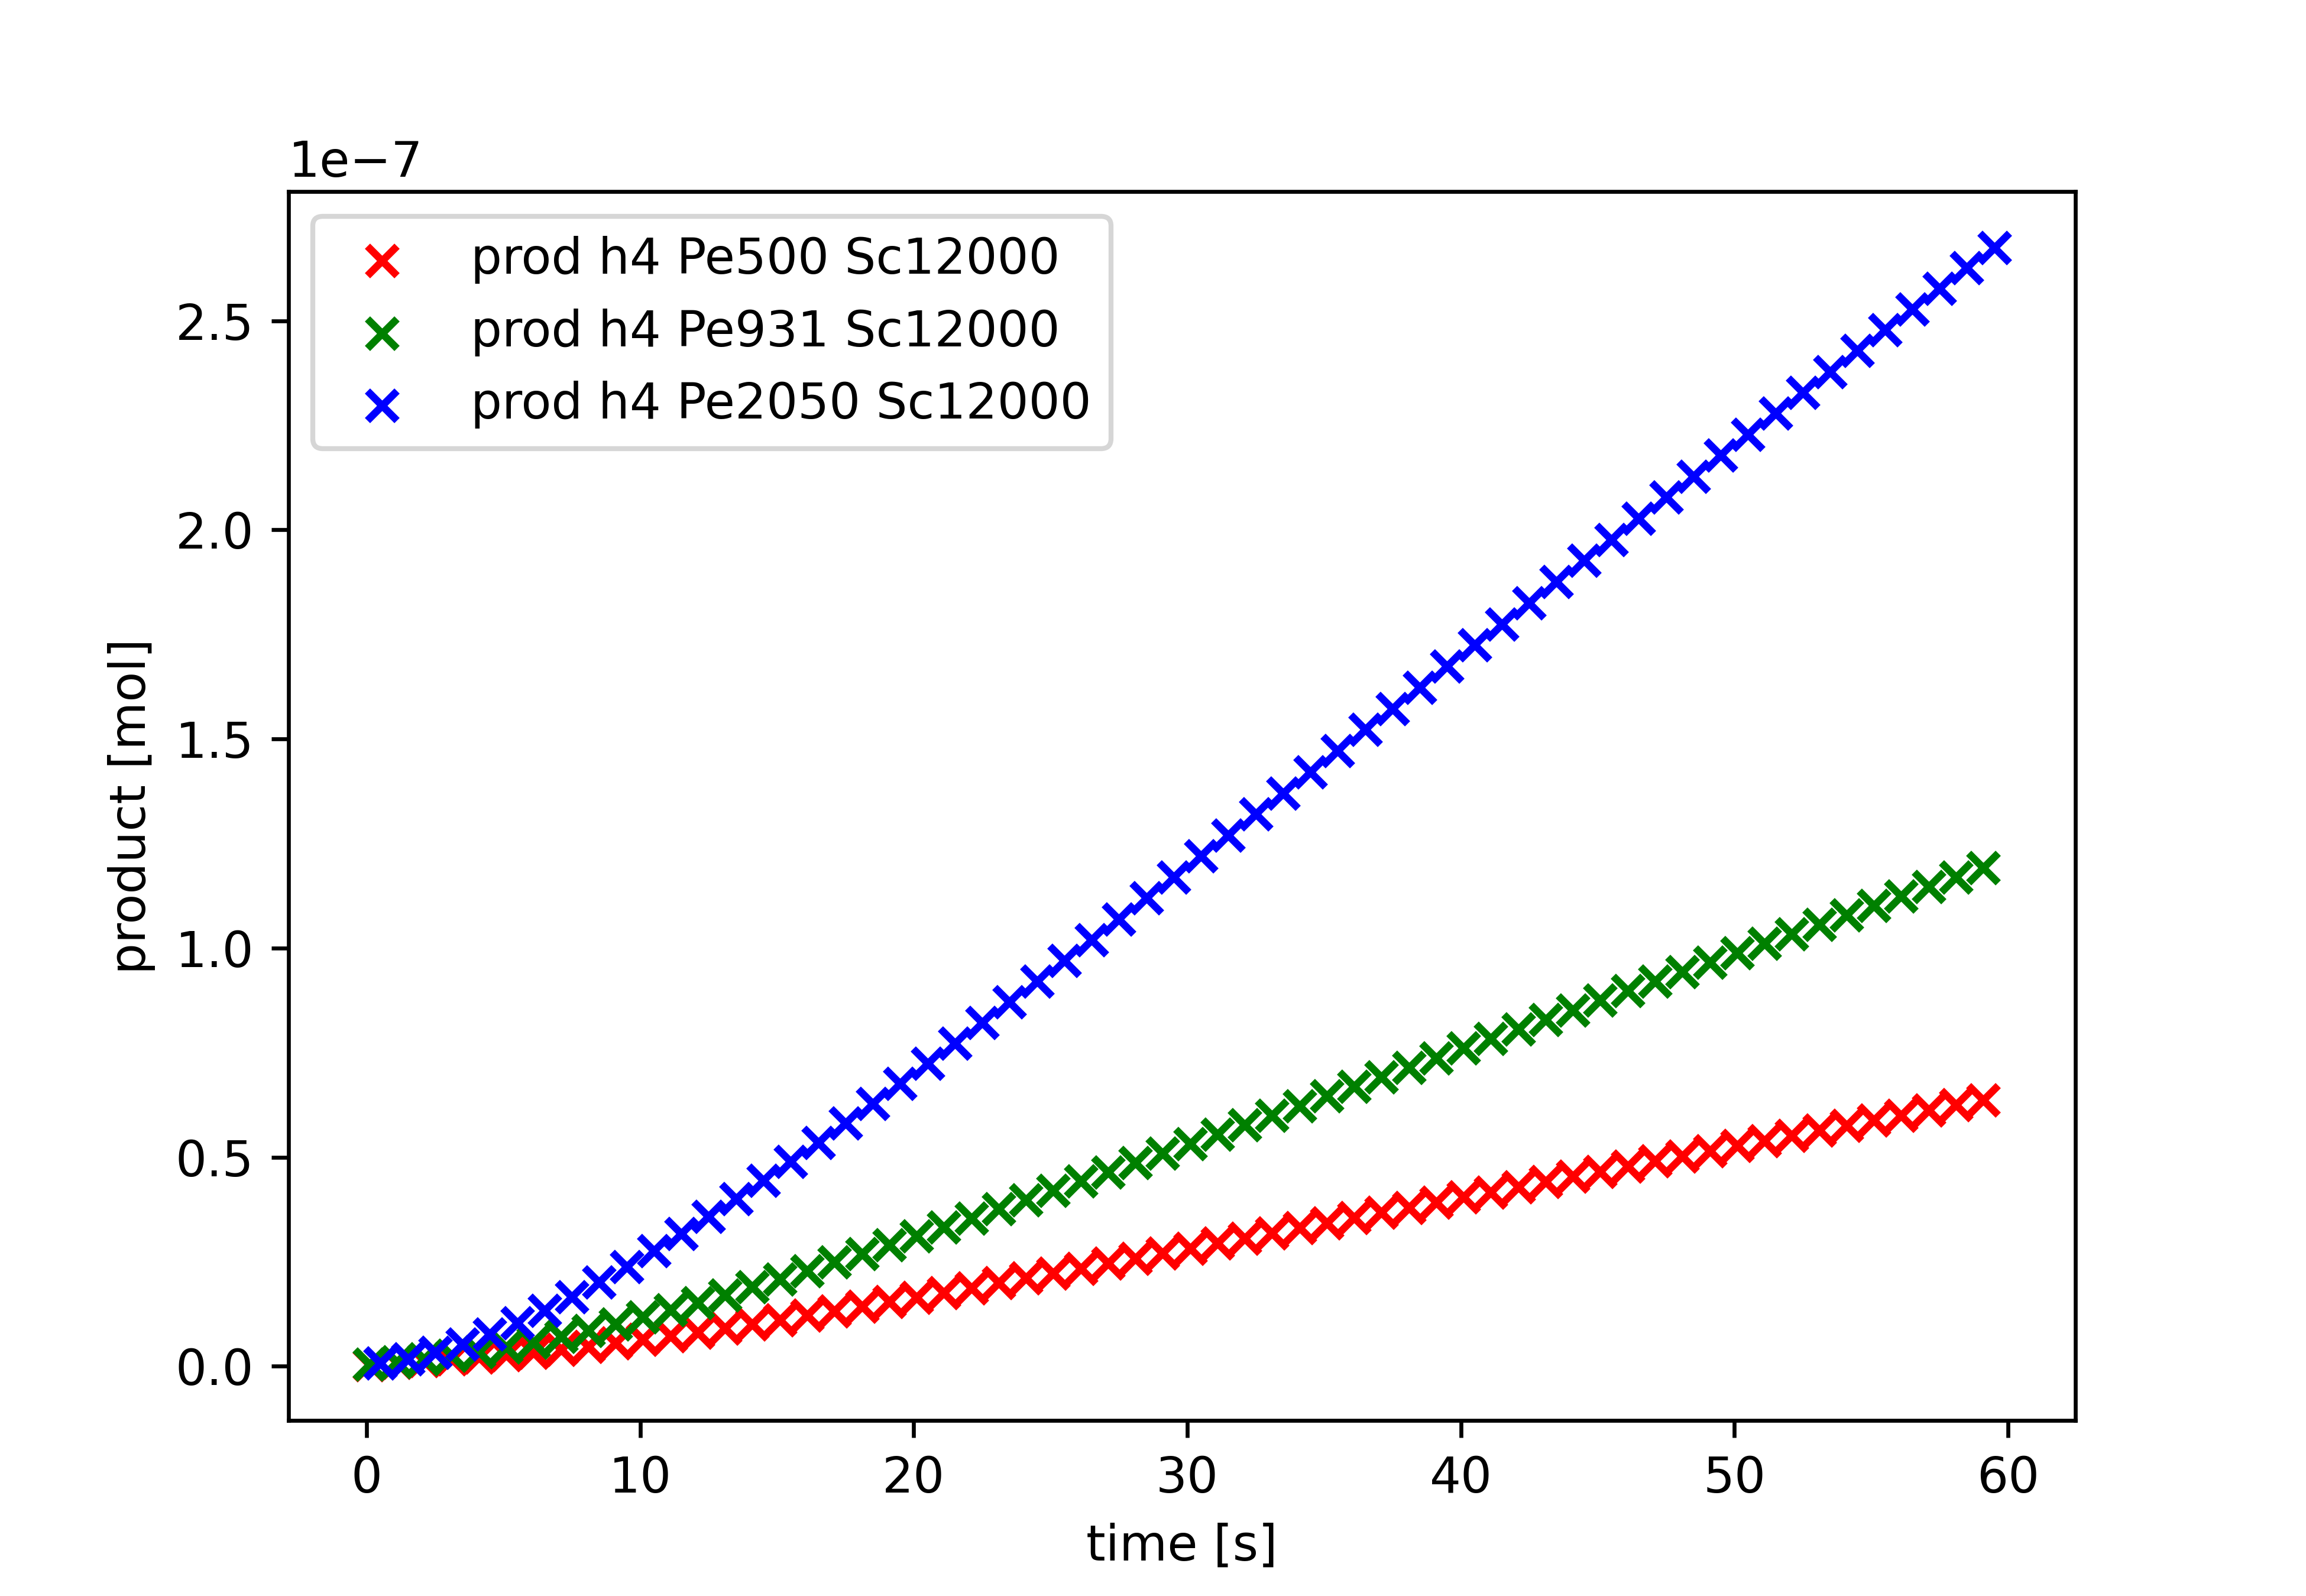
\includegraphics[width=.9\linewidth]{total_product_h4_Sc12000}
	\caption{Total product for  h = 0.4mm Sc = 12000}
	\label{fig: total_prod_h4_Sc12000}
\end{figure}
For the higher Schmidt number cases the total amount of product grows slowly in the first few seconds, but then increases linearly until the end for all cases. The production rate reached at the end is higher for higher Peclet numbers. 
\begin{figure}[htb]
	\centering
	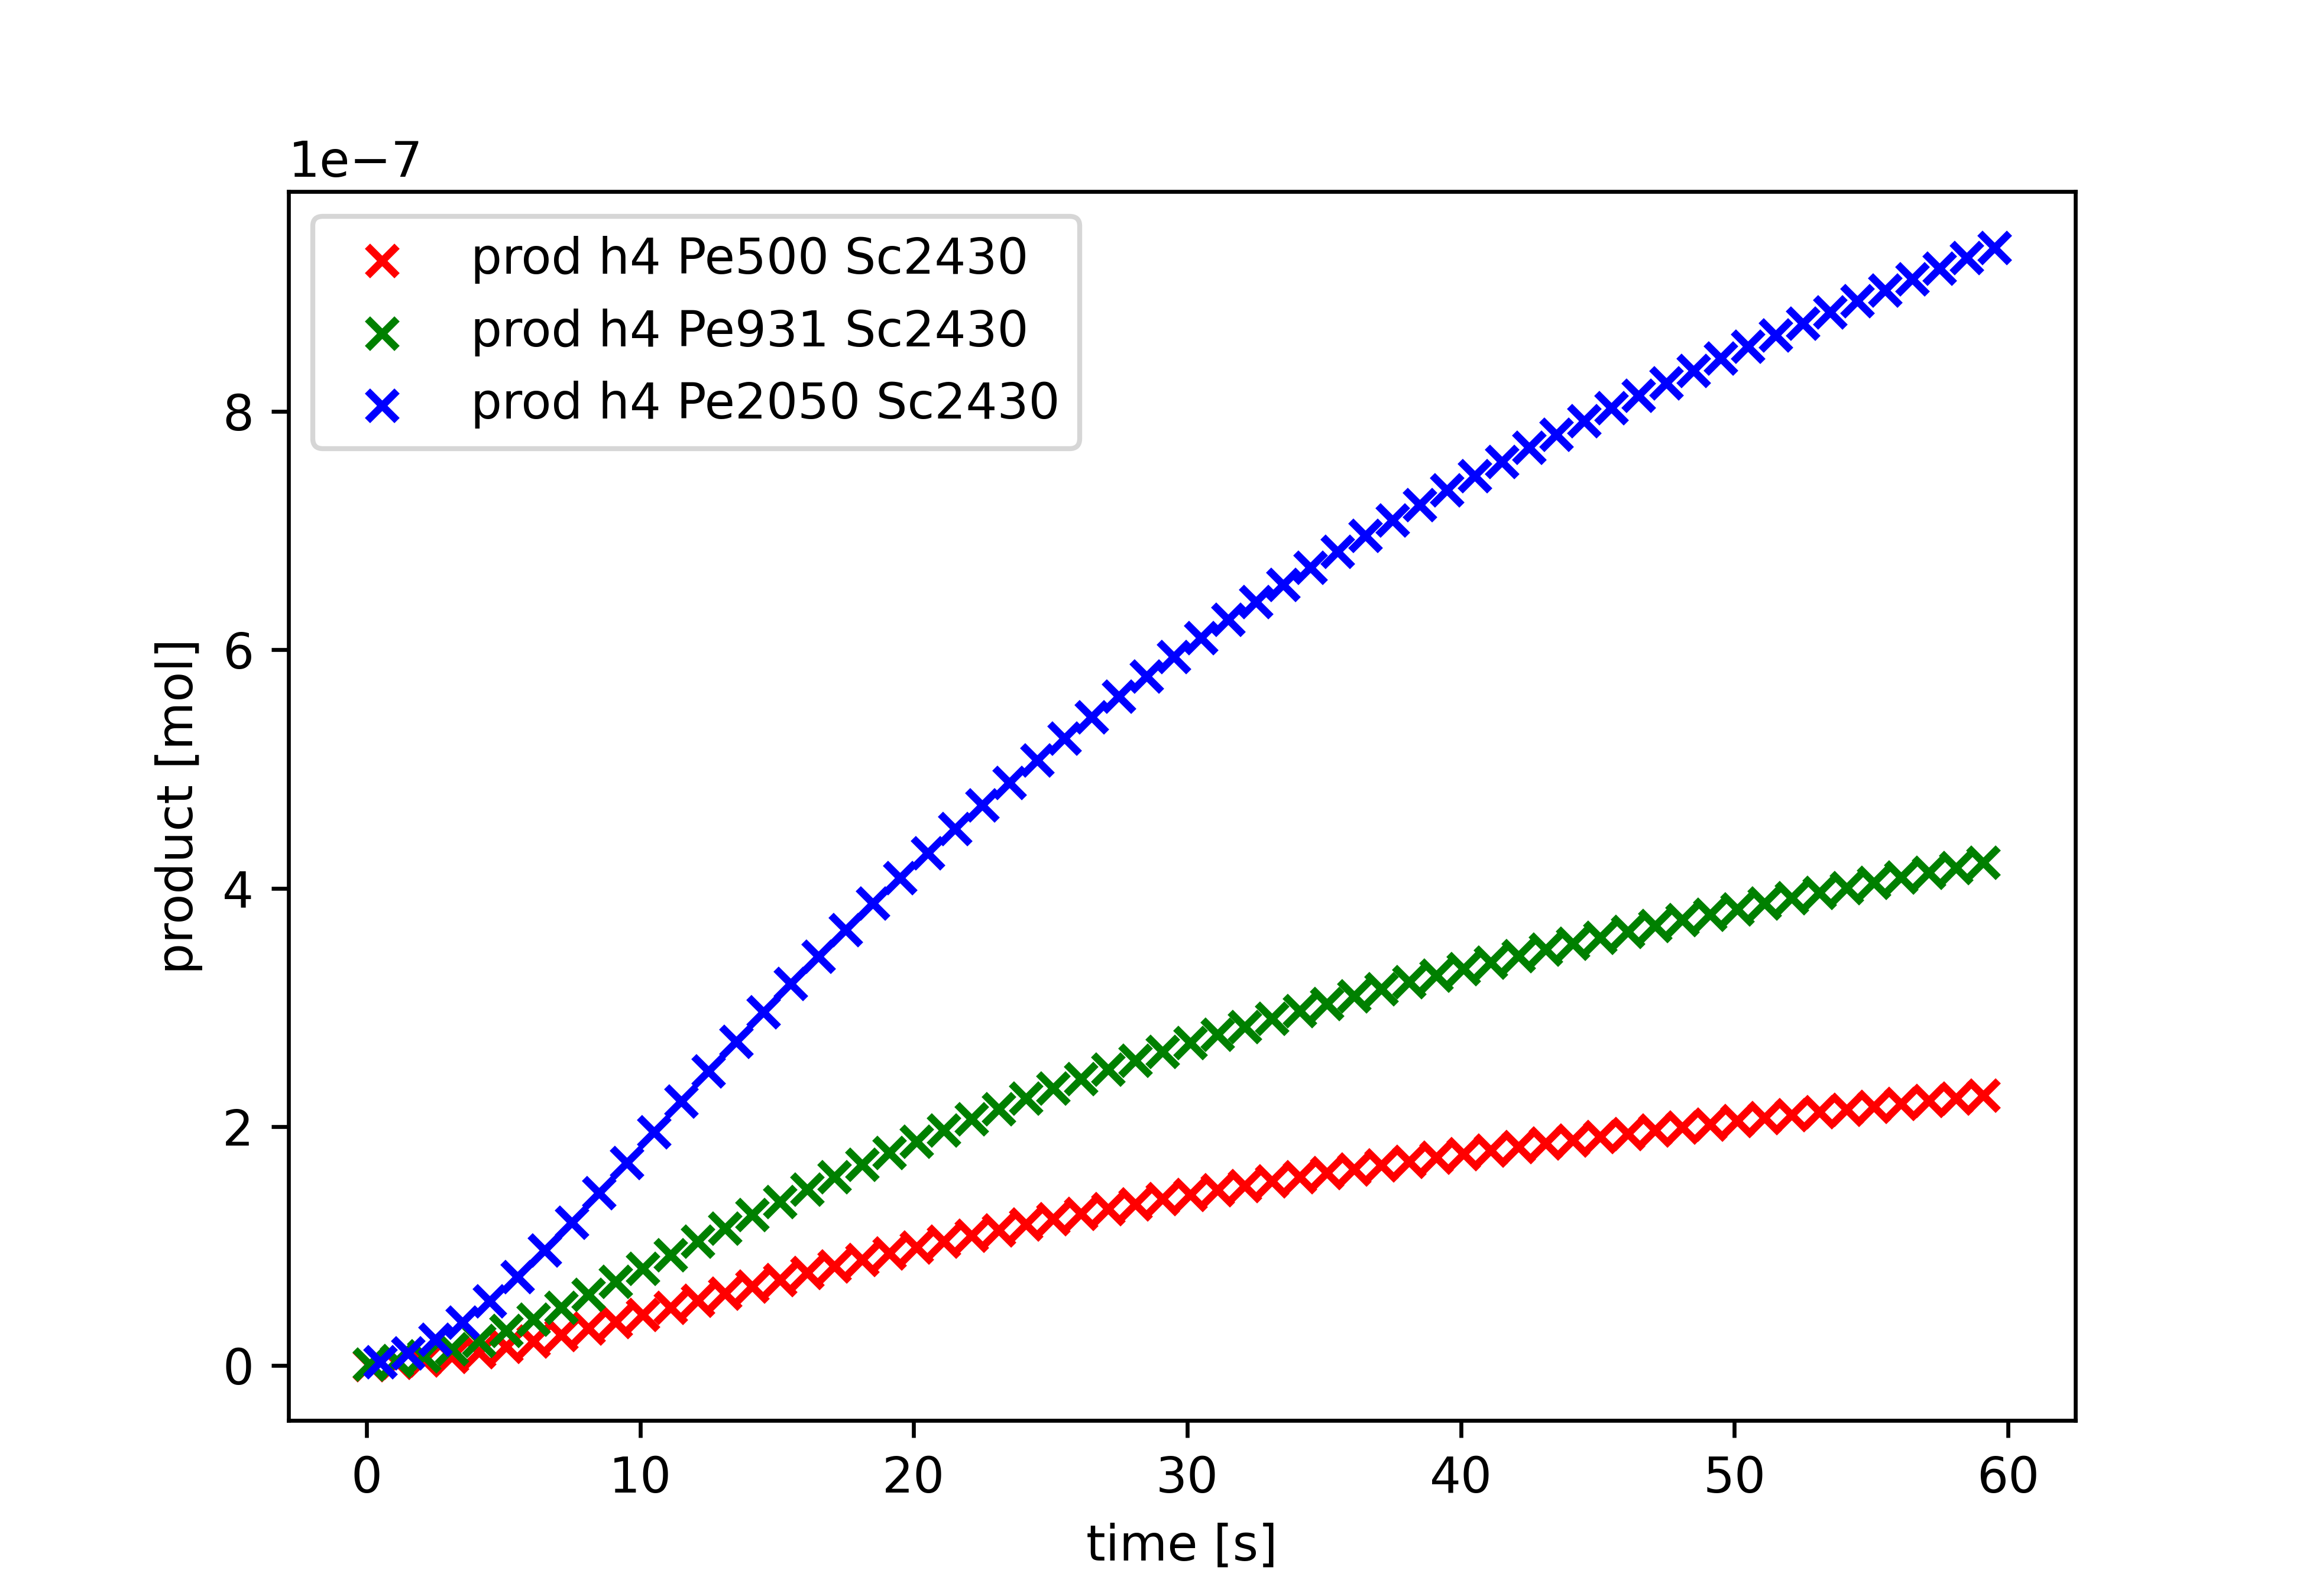
\includegraphics[width=.9\linewidth]{total_product_h4_Sc2430}
	\caption{Total product for  h = 0.4mm Sc = 2430}
	\label{fig: total_prod_h4_Sc2430}
\end{figure}

For the lower Schmidt number the graphs look very similar when comparing \autoref{fig: total_prod_h4_Sc2430} and \autoref{fig: total_prod_h2_Sc2430}. The values are higher for the 0.4mm case, but that is a result of the higher gap height and therefore higher volumetric flow through the reactor.

The amount of product created is highly influenced by the Peclet number. With approximately doubling the Peclet number between different cases for the same Schmidt number, the total product produced at 60 seconds goes up by a bit more than a factor of 2. That can be seen when comparing the cases for all different gap heights. That results are directly linked to the different input velocities that can be taken from \autoref{tab: cases}.

The cases with a gap height of 0.6mm and a Schmidt number of 12000 are still in the phase of higher production rate throughout the hole simulation run. In \autoref{fig: h6_late_shapes} the front shapes are shown for a time of 60 seconds for both Schmidt numbers.
\begin{figure}[htb]
	\centering
	\subfloat[\centering Sc=2430]{{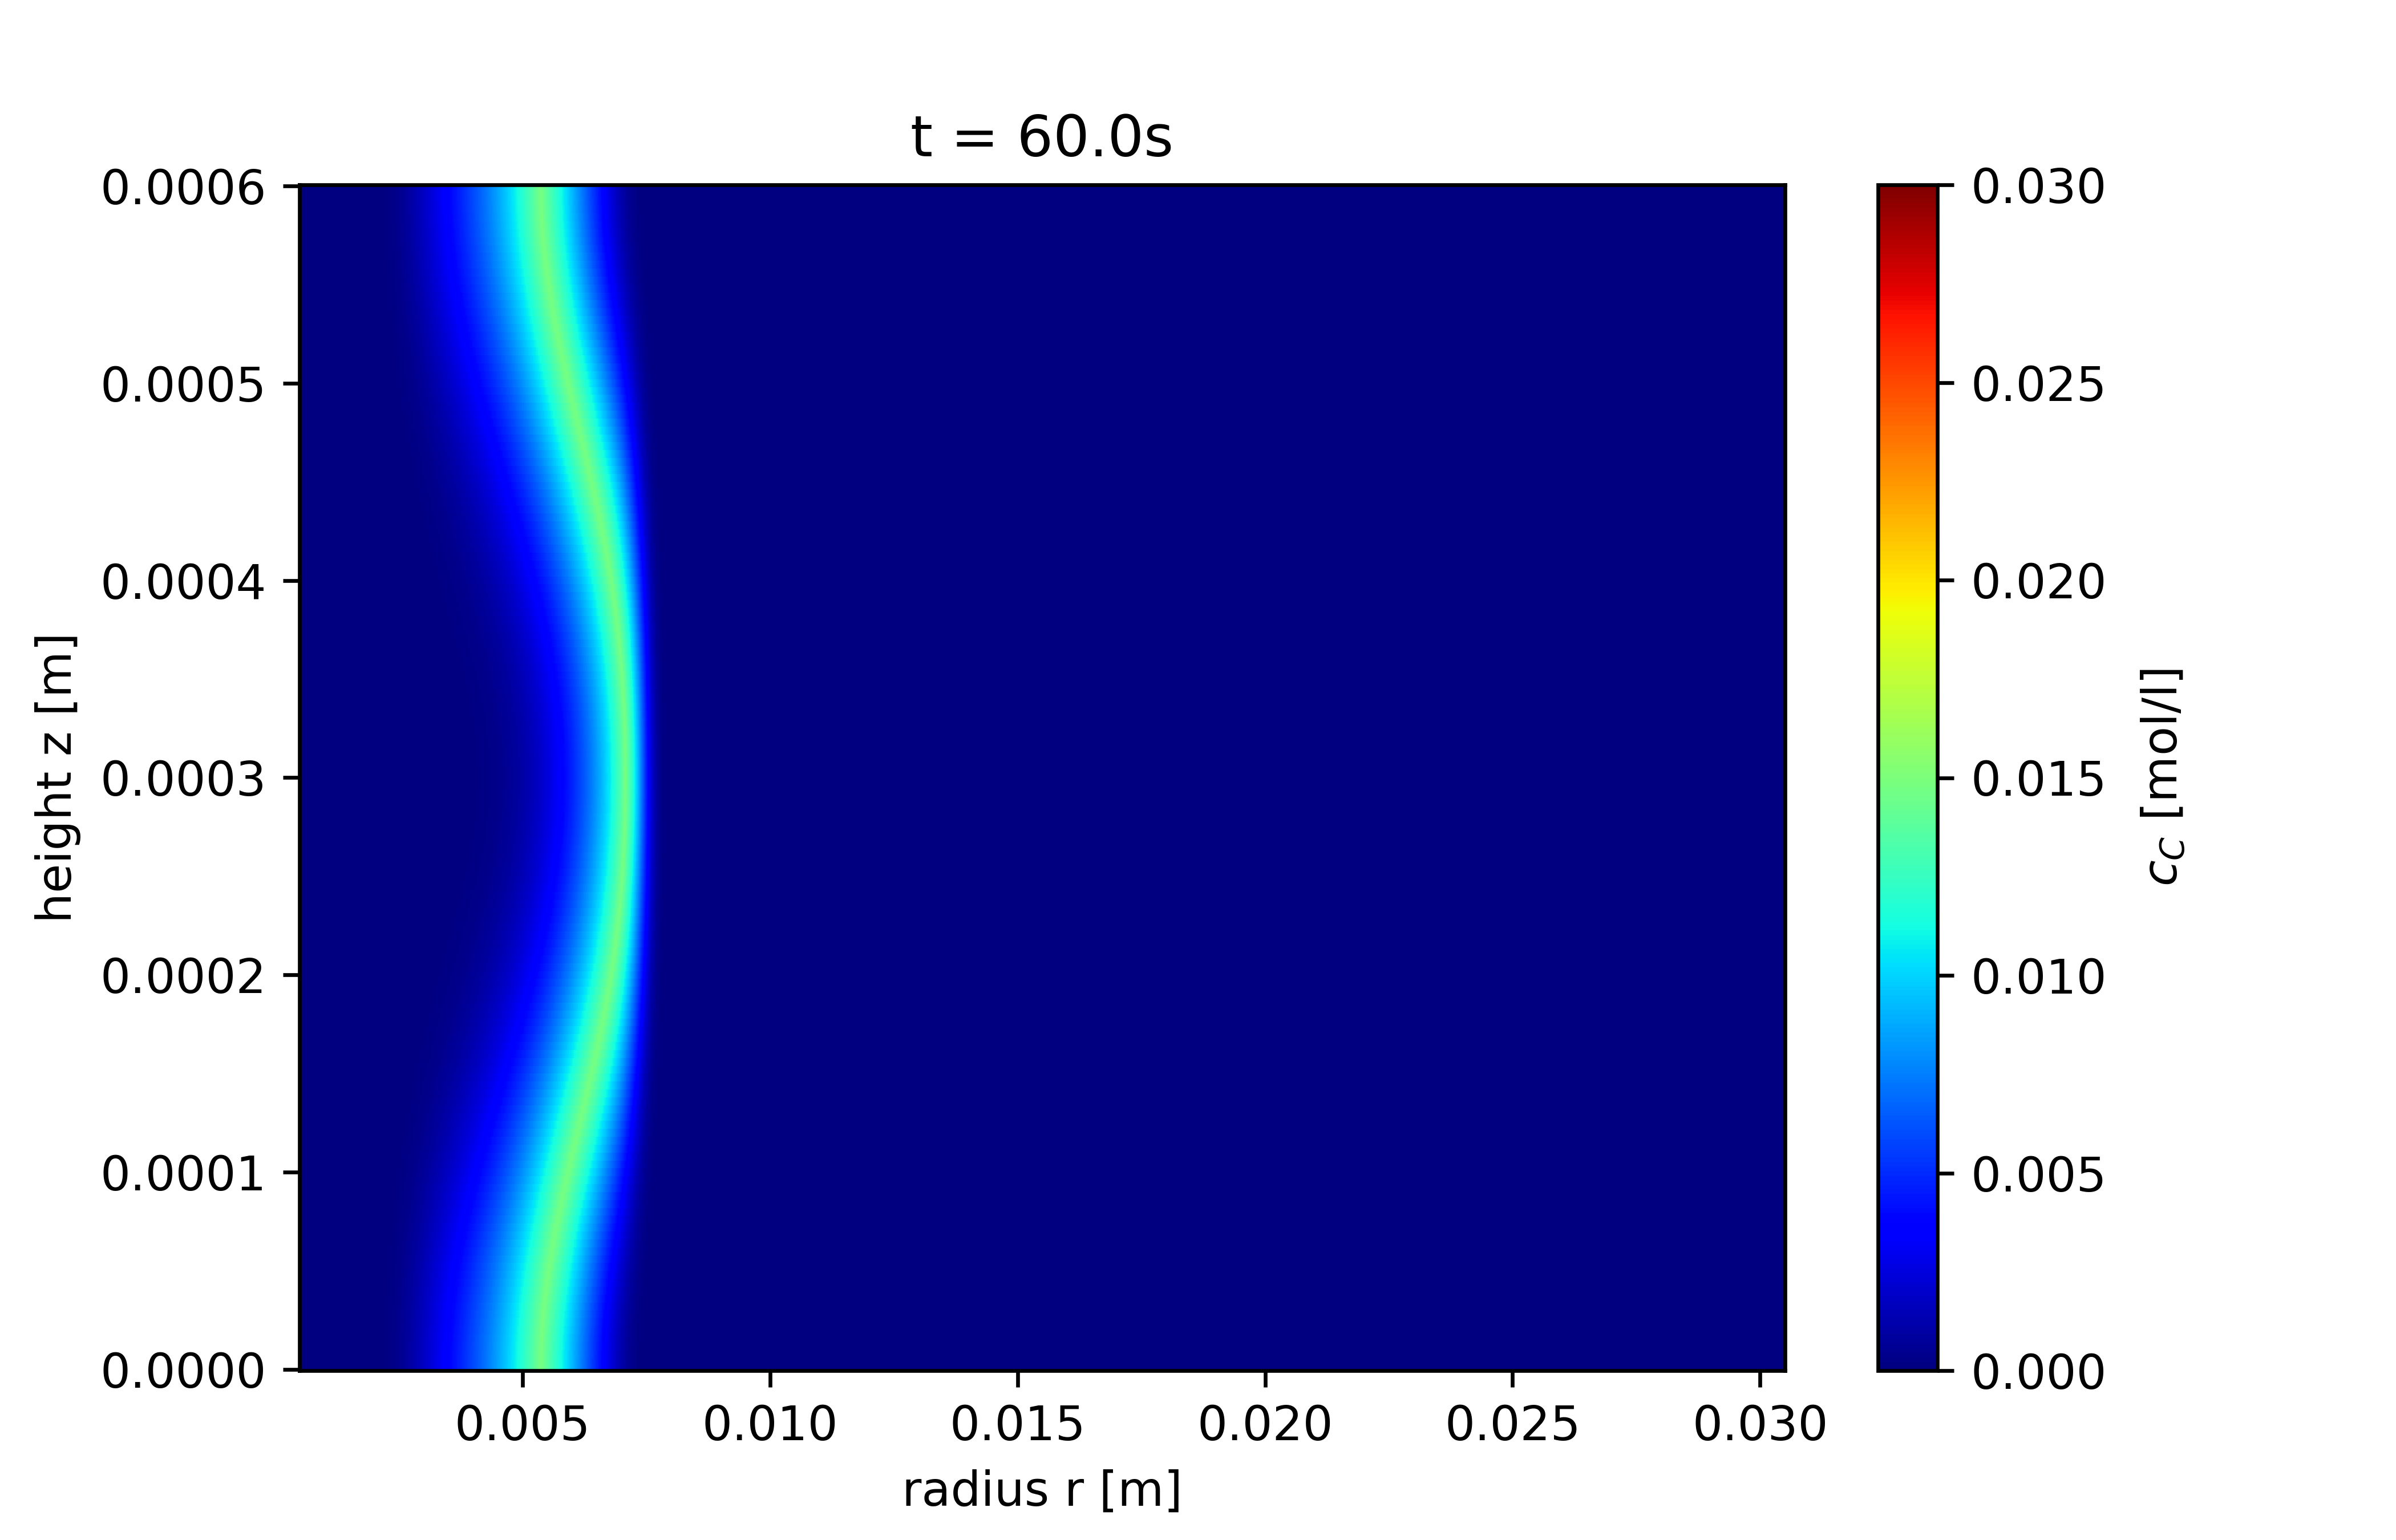
\includegraphics[angle=0, scale=0.41]{field_h6r3_P931E2_S243E3_concentration-fluid_c} }}%
	\qquad
	\subfloat[\centering Sc=12000]{{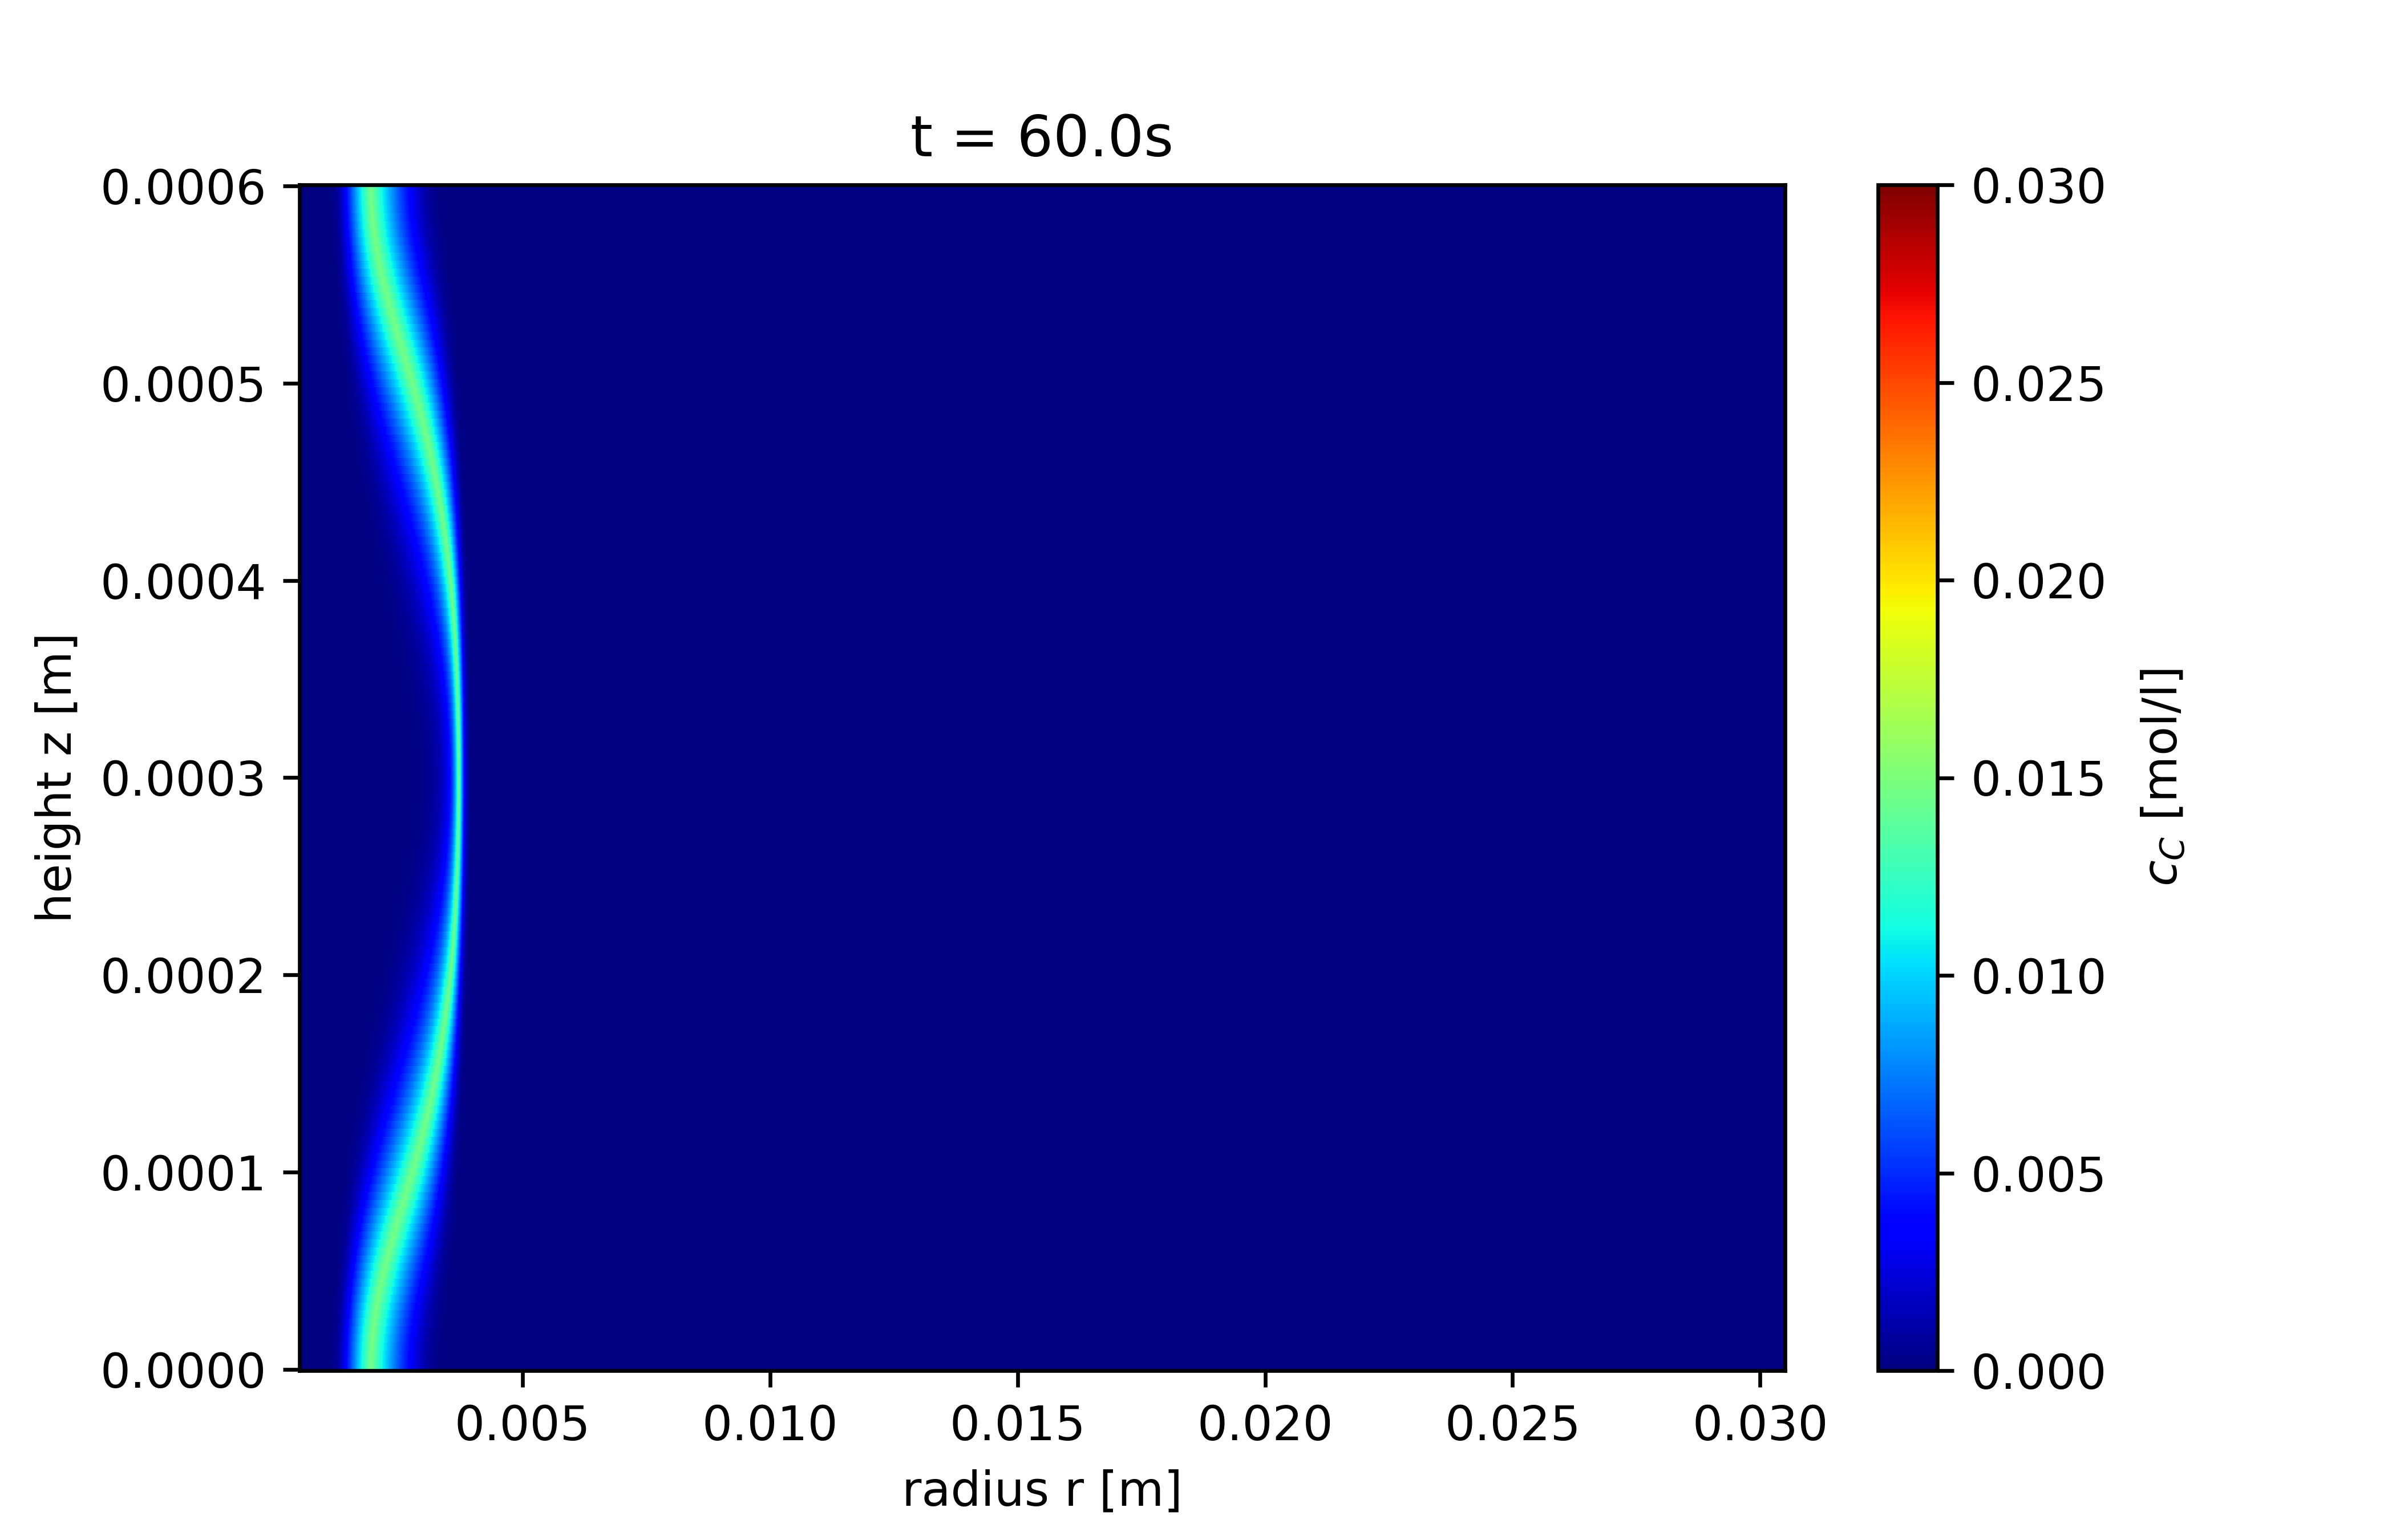
\includegraphics[angle=0, scale=0.41]{field_h6r3_P931E2_S120E4_concentration-fluid_c} }}%
	\caption{Product concentration fields at t = 60s for  h = 0.6mm  Pe = 931}%
	\label{fig: h6_late_shapes}%
\end{figure}
From the image showing the higher Schmidt number case it can be seen that the front is still building over the hole gap height, so the reaction rate would remain high until that is accomplished. A initial high production rate that after a while decreases can also be seen in the theoretical model developed by \cite{comolli2021dynamics}. Comparing to their work, the cases for the high Schmidt number and a gap height of 0.4mm and 0.6mm seem to be in the proposed early time regime \cite{comolli2021dynamics}.
Comparing that to the lower Schmidt number case were the front has nearly reached its final form, only a slight decay is visible towards the end of the simulation. To get clearer evidence on when the production rate has reached its final constant value the simulations need to be run for longer durations.

In \autoref{tab: prod_rates} all rates calculated by the linear fitting operation are shown.
\begin{table} [htb]
	\centering
	\caption{Production rates for all cases from linear fit}
	\begin{tabular}{ cccc }
		\hline
		gap height [mm] & Pe & Sc & $m$ [mol/s] \\
		\hline
		0.2 & 500 & 12000 & 5.815e-10 \\
		0.2 & 931 & 12000 & 1.064e-09 \\
		0.2 & 2050 & 12000 & 2.313e-09 \\
		0.2	& 500 & 2430 & 1.135e-09 \\
		0.2	& 931 & 2430 & 1.994e-09 \\
		0.2	& 2050 & 2430 & 4.136e-09 \\
		0.4 & 500 & 12000 & 1.215e-10 \\
		0.4 & 931 & 12000 & 2.255e-09 \\
		0.4 & 2050 & 12000 & 4.965e-09 \\
		0.4	& 500 & 2430 & 2.397e-09 \\
		0.4	& 931 & 2430 & 4.317e-09 \\
		0.4	& 2050 & 2430 & 9.242e-09 \\
		0.6 & 500 & 12000 & 1.196e-09 \\
		0.6 & 931 & 12000 & 2.246e-09 \\
		0.6 & 2050 & 12000 & 4.988e-09 \\
		0.6	& 500 & 2430 & 4.551e-09 \\
		0.6	& 931 & 2430 & 8.452e-09 \\
		0.6	& 2050 & 2430 & 1.874e-08 \\
		\hline
		\label{tab: prod_rates}
	\end{tabular}
\end{table}

The production rate shows a similar behaviour on a principle level within all investigated reactor geometries. The stages the fronts pass through in the 60 second time span of the simulation are different for the different gap heights.

\end{document}